%!TEX root=main.tex


%!TEX root = ../main.tex

\section{Introduction}
\label{s:intro}

Data errors are a pervasive, expensive, and time consuming problem
that afflicts the vast majority of data-driven applications. For
example, errors in retail price data cost US consumers \$2.5 billion
each year~\cite{Fan2008}. In aggregate, studies estimate data errors
to cost the US economy more than \$600 billion per
year~\cite{eckerson2002}. Therefore, it is not surprising that a
significant fraction of time in data analysis --- up to
80\%~\cite{kandel2012} --- is devoted to cleaning and
wrangling~\cite{kandel2011wrangler} the data into a structured and
sufficiently clean form to use in downstream applications.

In response, both industry and academia has focused on data cleaning solutions to mitigate this problem.
ETL-type systems~\cite{systemt, informatica} focus on cleansing the data before it is loaded into the database
using a set of pre-defined rules; outlier and anomaly detection algorithms~\cite{} are used to identify errors
in the database after the data has been loaded; while recent approaches use downstream applications
such as interactive visualizations, application queries, or data-products to facilitate error detection and correction algorithms.
In each of these cases, the focus of error diagnosis and cleaning has been {\it data centric}, in the sense that
the process is meant to identify and directly fix data values.

These efforts have largely ignored an important source of data errors --- data modification {\it queries}.
Mistakes in such queries can introduce errors that spread throughout the database due to subsequent, possibly correct updates.
Consider the following salary management example:

% change example
%!TEX root = ../main.tex


\begin{figure*}[t]
    \begin{minipage}[t]{0.28\textwidth}
         \vspace{0pt} 
         \centering
        \begin{tabular}{llll}
            \multicolumn{4}{l}{\emph{Taxes}: $D_0$}\\
            \toprule
            \textbf{ID}  & \textbf{income}    & \textbf{owed} & \textbf{pay} \\
            \midrule
            $t_1$   & \$9500    & \$950		& \$8550 \\
            $t_2$   & \$90000   & \$22500 	& \$67500\\
            $t_3$   & \$86000   & \$21500	& \$64500\\
            $t_4$   & \$86500   & \$21625	& \$64875\\
            \bottomrule
            \\
        \end{tabular}
    \end{minipage}
    \begin{minipage}[t]{0.43\textwidth}
         \vspace{0pt} 
         \centering
        \begin{tabular}{|p{1ex}l|}
            \multicolumn{2}{l}{\emph{Query log}: $\mathcal{Q}$}\\
            % \toprule
            \hline
            
            $q_1$: & \texttt{\small UPDATE Taxes SET owed=income*0.3}\\
            	   & \texttt{\small WHERE income>=\color{red}{85700}}\\
            
            $q_2$: & \texttt{\small INSERT INTO Taxes}\\ 
                   & \texttt{\small VALUES (25, 85800, 21450)}\\
                   
            $q_3$: & \texttt{\small UPDATE Taxes SET pay=income-owed}\\ 
            \hline
            % \bottomrule
        \end{tabular}
    \end{minipage}
    \begin{minipage}[t]{0.28\textwidth}
         \vspace{0pt} 
         \centering
        \begin{tabular}{llll}
            \multicolumn{4}{l}{\emph{Taxes}: $D_4$}\\
            \toprule
            \textbf{ID}  & \textbf{income}    & \textbf{owed}  & \textbf{pay}\\
            \midrule
            $t_1$ & \$9500    & \$950		& \$8550\\
            $t_2$   & \$90000   & \$27000	& \$63000\\
            \rowcolor{mid-gray}
            $t_3$ & \$86000   & \color{red}{\$25800} & \color{red}{\$60200}\\
            \rowcolor{mid-gray}
            $t_4$	 & \$86500	  & \color{red}{\$25950}	& \color{red}{\$60550}\\
            $t_5$	 & \$87000	  & \$21750	& \$65250\\
            \bottomrule
        \end{tabular}
    \end{minipage}

    \caption{A recent change in tax rate brackets calls for a tax rate of 30\% for those with income above \$87500.  The accounting department issues query $q_1$ to implement the new policy, but the predicate of the WHERE clause condition transposed two digits of the income value.
\iffalse  
As a result, the owed amount of $t_3$ and $t_4$ were calculated incorrectly. 
This mistake is obscured by $q_2$ which insert a tuple with correct income and owed amount and later further propagated to additional filed(s) by query $q_3$ which calculates the pay check amount based on the corresponding income and (incorrect) owed values.
\fi
    % \alex{I am confused about what happened with this example.  The numbers in the figure don't match the description in Example 3.  This doesn't see to be used later (yet).  Before I fix it, I want to check whether there is a reason for the particular changes...}}\xlw{I changed this example for later optimization sec.6 and noise sec.7 handling explanation. There are two goals: 1. we will demonstrate why we need 2 iterations to reduce noise when we only encode tuples in the complaint set for efficiency; 2. we will show if how we detect and prune false positive complaint $t_5$ by constructing complaint-tuple bipartite graph and searching densest sub-graph. 
    }
    \label{fig:example}
\end{figure*}
%%!TEX root = ../main.tex


\begin{figure*}[t]
    \begin{minipage}[t]{0.28\textwidth}
         \vspace{0pt} 
         \centering
        \begin{tabular}{llll}
            \multicolumn{4}{l}{\emph{Taxes}: $D_0$}\\
            \toprule
            \textbf{ID}  & \textbf{income}    & \textbf{owed} & \textbf{pay} \\
            \midrule
            $t_1$   & \$9500    & \$950		& \$8550 \\
            $t_2$   & \$90000   & \$22500 	& \$67500\\
            $t_3$   & \$86000   & \$21500	& \$64500\\
            $t_4$   & \$86500   & \$21625	& \$64875\\
            \bottomrule
            \\
        \end{tabular}
    \end{minipage}
    \begin{minipage}[t]{0.43\textwidth}
         \vspace{0pt} 
         \centering
        \begin{tabular}{|p{1ex}l|}
            \multicolumn{2}{l}{\emph{Query log}: $\mathcal{Q}$}\\
            % \toprule
            \hline
            
            $q_1$: & \texttt{\small UPDATE Taxes SET owed=income*0.3}\\
            	   & \texttt{\small WHERE income>=\color{red}{85700}}\\
            
            $q_2$: & \texttt{\small INSERT INTO Taxes}\\ 
                   & \texttt{\small VALUES (25, 85800, 21450)}\\
                   
            $q_3$: & \texttt{\small UPDATE Taxes SET pay=income-owed}\\ 
            \hline
            % \bottomrule
        \end{tabular}
    \end{minipage}
    \begin{minipage}[t]{0.28\textwidth}
         \vspace{0pt} 
         \centering
        \begin{tabular}{llll}
            \multicolumn{4}{l}{\emph{Taxes}: $D_4$}\\
            \toprule
            \textbf{ID}  & \textbf{income}    & \textbf{owed}  & \textbf{pay}\\
            \midrule
            $t_1$ & \$9500    & \$950		& \$8550\\
            $t_2$   & \$90000   & \$27000	& \$63000\\
            \rowcolor{mid-gray}
            $t_3$ & \$86000   & \color{red}{\$25800} & \color{red}{\$60200}\\
            \rowcolor{mid-gray}
            $t_4$	 & \$86500	  & \color{red}{\$25950}	& \color{red}{\$60550}\\
            $t_5$	 & \$87000	  & \$21750	& \$65250\\
            \bottomrule
        \end{tabular}
    \end{minipage}

    \caption{A recent change in tax rate brackets calls for a tax rate of 30\% for those with income above \$87500.  The accounting department issues query $q_1$ to implement the new policy, but the predicate of the WHERE clause condition transposed two digits of the income value.
\iffalse  
As a result, the owed amount of $t_3$ and $t_4$ were calculated incorrectly. 
This mistake is obscured by $q_2$ which insert a tuple with correct income and owed amount and later further propagated to additional filed(s) by query $q_3$ which calculates the pay check amount based on the corresponding income and (incorrect) owed values.
\fi
    % \alex{I am confused about what happened with this example.  The numbers in the figure don't match the description in Example 3.  This doesn't see to be used later (yet).  Before I fix it, I want to check whether there is a reason for the particular changes...}}\xlw{I changed this example for later optimization sec.6 and noise sec.7 handling explanation. There are two goals: 1. we will demonstrate why we need 2 iterations to reduce noise when we only encode tuples in the complaint set for efficiency; 2. we will show if how we detect and prune false positive complaint $t_5$ by constructing complaint-tuple bipartite graph and searching densest sub-graph. 
    }
    \label{fig:example}
\end{figure*}

Although existing data-centric cleaning techniques may help identify and correct these reported errors directly, 
this is suboptimal because it treats the symptom --- the errors in the current database state --- rather than the anomalous
queries that are the underlying cause.  In practice, only a subset of the paystub errors will be reported, thus fixing
the reported errors on a case-by-case basis will likely obscure the root problem, making it more difficult to
find both the erroneous query and the other affected data.  
Furthermore, a data-centric approach must repair \emph{all errors} --- a non-repaired value such as the incorrect tax rate
may continue to introduce errors in the database through future queries 
(e.g., inserting incorrectly computed paychecks based on the still-incorrect tax rate).

\alex{Leaving this paragraph to Eugene.}
For these reasons, traditional data cleaning approaches may be helpful for finding errors in the data, but are
not designed to diagnose causes of the errors when they are rooted in incorrect queries.
There has been some work, but not directly for this problem.  
\ewu{fill in with related work}
Integrity constraints.
Certificate-based verification.
Structural sources of mistakes, but not identify the specific faulty query and how it is wrong.
In more restricted domains, data explanation finds predicates to exclude from queries, but only work for a single, simple  aggregation query.

Query-centric cleaning and repair is challenging because an error introduced by a query can be obscured by, or propagated throughout the database
by subsequent queries. This alludes to several factors that make even identifying problematic queries difficult:

\begin{enumerate}[leftmargin=*, topsep=0mm, itemsep=0mm]

  \item \textbf{Butterfly fffect: } 
  An error in even a single query can affect a large number of records, as documented in several real-world
  cases~\cite{Yates10, Grady13, sakalerrors}.  Even if a single record is incorrect,
  its value may be used as part of the \texttt{WHERE} or \texttt{SET} clauses of 
  subsequent valid queries that introduce additional errors that are seemingly unrelated.

  \item \textbf{Partial information:}  In most practical settings, we cannot assume that we can identify all
  errors in the database --- for example, not all employees will complain about their incorrect paystubs.  
  More likely, we only have access to a subset of the data errors, and must use them to extrapolate 
  the queries that affected a possibly larger set of data.  A diagnostic tool that can reduce
  the entire transaction log to the most likely candidate queries and propose fixes
  is needed to make this process manageable.


  \item \textbf{Multiple types of errors:} 
  An erroneous query can cause multiple types of data errors.  For example, a record that should not exist may have been accidentally inserted, or conversely a record that 
  should exist was unintentionally deleted.  Similarly, attribute values may be incorrectly updated,
  updated when they should not have been, or not updated when they should have.  
  Any combination of these error types may be present in the current state of the database,
  and although they may not be obviously related to each other, they must be addressed in a holistic manner.  

\end{enumerate}


In this demo proposal, we outline the design of \sys, a framework that derives explanations
and repairs for discrepancies in relational data based on potential errors in
the queries that operated on the data, and describe how users will use \sys
in a demonstration scenario. 
In contrast to existing approaches in data
cleaning that aim to detect and correct errors in the data directly, the goal
of \sys is to identify  the problematic queries that introduced errors into the
database. These diagnoses both \emph{explain} how errors were introduced to a
dataset, and also lead to the identification of additional discrepancies in
the data that would have otherwise remained undetected.
Participants will be able to 
select from a number of transactional benchmarks to generate a query workload,
introduce errors into the queries that are executed,
and compare the fixes to the queries proposed by \sys against existing alternative algorithms such as decision trees.



% Poor data quality is a hard and persistent problem.  It is estimated to cost the US economy more than \$600 billion
% per year~\cite{eckerson2002} and erroneous price data in retail databases
% alone cost the US consumers \$2.5 billion each year~\cite{Fan2008}. Although data
% cleaning tools can purge many errors from a dataset before downstream 
% applications use the data, databases are constantly changing as applications
% and users execute queries that modify the data.
% Mistakes in these queries can introduce errors that spread through the database
% due to subsequent update queries; 
% by the time errors are detected, it is difficult to trace those errors back to the 
% erroneous query and correct it.
% Identifying and correcting errors in the data directly is suboptimal: it treats the symptom,
% rather than the underlying cause. Fixing the manifested data errors on a
% case-by-case basis often obscures the root of the problem and other data that may have been
% affected. Therefore, traditional data cleaning approaches are not well-suited
% for this setting: While they provide general-purpose tools to identify and
% rectify anomalies in the data, they are not designed to diagnose the causes of
% errors that are rooted in erroneous updates.
% Some data cleaning systems try to identify structural sources of
% mistakes~\cite{wang2015}, but they are unable to trace the source of
% the mistakes to particular faulty queries.
% 
% While improving data quality and correcting data errors has been an important
% focus for data management research, handling new errors, introduced during
% regular database interactions, has received little attention. Most work in
% this direction focuses on \emph{guarding against} erroneous updates. For
% example, integrity constraints~\cite{Khoussainova2006} reject some improper
% updates, but only if the data falls outside rigid, predefined ranges.
% Certificate-based verification~\cite{Chen2011} is less rigid, but it is
% impractical and non-scalable as it requires users to answer challenge
% questions before allowing the updates, and it is not applicable to updates
% initiated by applications.





% \begin{example}[Wireless discount policies]\label{ex:telco}
% 
% A large US-based wireless provider offers company discounts as incentives for
% corporate customers. There are different types of discounts (flat, percentage,
% fee-based), and their details are specific to corporate agreements. The large
% number of policies and complexities in their rules frequently cause policies
% to be set incorrectly, leading to errors in the application of discounts to
% customers' accounts.
% 
% Customers who notice billing errors contact the provider, but the call centers
% do not have the capacity or ability to investigate the complaints deeply. The
% standard course of action is to correct billing mistakes on a case-by-case
% basis for each complaint. As a result, unreported errors remain in the
% database for a long time, or they never get corrected, and their cause becomes
% harder to trace as the source of the errors is obscured.\footnote{This is a real-life scenario, provided to us by a popular US-based wireless provider.}
% 
% \end{example}

% \begin{example}[Tax bracket adjustment]\label{ex:taxes}
%     
% Tax brackets, which determine tax rates for different income levels, are
% often adjusted. Accounting firms implement these changes to their
% databases by appropriately updating the tax rates of their customers. Mistakes
% in these update queries (e.g., Figure~\ref{fig:example}) result in errors in
% the tax rates and computed taxes. 
% 
% \end{example}
% 
% 
% In this application, data errors are typically reported to a
% customer service department, which does not have the resources nor the
% capability to investigate the errors more broadly. Instead, errors are
% resolved on a case-by-case basis. In practice, customer service only deals
% with a small portion of the actual errors. Once these errors are resolved,
% there will still be a large number of incorrect records that were not
% identified. The goal of \sys is to identify the query or queries that caused
% the errors, propose corrections to those queries, and use the modified queries
% to identify other errors.
% 
% Diagnosing data errors stemming from incorrect updates is fundamentally
% challenging: the search space of possible mistakes and fixes is large, and the
% amount of information (number of known errors) may be limited. The problem has
% the following important characteristics that render traditional data cleaning
% methods unsuitable:



% \begin{description}[leftmargin=*, topsep=0mm, itemsep=0mm]
%     
%     \item[Obscurity.] Detection of the resulting errors in the data often
%     leads to partial fixes that further complicate the eventual diagnosis and
%     resolution of the problem. For example, a transaction implementing a
%     change in the state tax law updated tax rates using the wrong rate,
%     affecting a large number of consumers. This causes a large number of
%     complaints to a call center, but each customer agent usually fixes each
%     problem individually, which ends up obscuring the source of the problem.
%     
%     \item[Large impact.] Erroneous queries cause errors at a large scale. The
%     potential impact of the errors is high, as manifested in several
%     real-world cases~\cite{Yates10, Grady13, sakalerrors}. Further, errors
%     that remain undetected for a significant amount of time can instigate
%     additional errors, even through valid updates. This increases both their
%     impact, and their obscurity.
%     
%     \item[Systemic errors.] The errors created by bad queries are
%     \emph{systemic}: they have common characteristics, as they share the same
%     cause. The link between the resulting data errors is the query that
%     created them; cleaning techniques should leverage this connection to
%     diagnose and fix the problem. Diagnosing the cause of the errors, will
%     achieve systematic fixes that will correct all relevant errors, even if
%     they have not been explicitly identified.
%    
% \end{description}
% 
% \sys addresses these challenges by analyzing the queries that operated on a
% dataset in an efficient and scalable manner. More concretely, we make the
% following contributions:


% The goal of this paper is to design effective query
% diagnosis techniques and identify possible fixes for query errors. We
% model the problem assuming a log of update workloads over a database,
% and a set of complaints that identify errors in the final database
% state. We organize our contributions as follows:

% \ewu{really like this organization}

% \ewu{add: special case optimizations for single query case.}


% \begin{itemize}[leftmargin=*, topsep=0mm, itemsep=0mm]      
%     \item We formalize the problem of diagnosing a set of errors using log
%     histories of updates that operated on the data. Given a set of 
%     \emph{complaints} as representations of data discrepancies in the current
%     state of a dataset, \sys identifies the queries in the log that require the  minimal
%     amount of changes that would resolve all of the complaints (Section~\ref{sec:abstractions}).
%       
%     \item We provide an exact error-diagnosis solution through a non-trivial
%     transformation of the problem to a mixed integer linear program (MILP) that
%     encodes the data provenance of the erroneous tuples. Our approach employs state-of-the-art MILP solvers to identify
%     optimal diagnoses that are guaranteed to resolve all complaints without introducing new errors to the data
%     (Section~\ref{sec:sol}).
%     
%     \item We present several optimizations to our basic diagnostic
%     method, which reduce the problem size without affecting the
%     quality of the produced solutions. Further, we propose an
%     incremental repair method that targets the cases where the log
%     contains a single corrupted query (or the search focuses on a
%     single repair). This incremental analysis of the log allows us to
%     scale to very large datasets and large query logs. Further, we
%     show that our optimization techniques have the additional
%     advantage of tolerating incomplete information, such as unreported
%     errors (Section~\ref{sec:opt}).
% 
%     
%     % \item We extend our framework to also handle false positives: complaints
%     % that mistakenly identify data as erroneous. We define the notion of
%     % complaint \emph{density}, which is a query-driven measure of closeness of
%     % a complaint to other complaints. The main intuition of our approach is
%     % that complaints of low density are likely false positives and thus can be
%     % safely ignored (Section~\ref{???}).
%     
%     \item We experimentally evaluate the effectiveness and efficiency of our
%     methods against real-world and synthetic datasets and query logs. 
%     (Section~\ref{sec:experiments}). 
% \end{itemize}

% 
\section{Real-world examples}
\label{s:usecase}

\alex{I am not convinced that these deserve a section.  It would make sense if we actually applied our system on them and had something to say about the derived diagnoses and fixes.  As they are, I would use as examples in the introduction instead.}

\subsection{Telco}

Call centers get customer complaints about billing all the time.
For example, there was a change in the tax law, but the transactions
that updated the taxes didn't change, so they would get lots of
customer complaints.  Each customer agent usually fixes each problem
individually, however, it's a system problem to all of Kansas that
usually doesn't get caught until late in the game.  In this case
it's a faulty update to a numerical value whose effects compound
over time.  There is external domain knowledge to isolate the
culprits to tax-related transactions, and sensitivity analysis can
be useful.

\subsection{Insurance}

A colleague recently switched to medicare but because of a problem
with the transactions to switch him from his previous to new
insurance, it's caused him 6 months of headaches.  3 months ago he
learned that a bunch of other people have been complaining about
the same issues regarding the switch.  In this case it's a categorical
change (from one insurance to another) that has more obvious impact.



%!TEX root = ../main.tex

\section{Modeling abstractions}
\label{sec:abstractions}

In this section, we introduce a running example inspired from the use-case of
Example~\ref{ex:taxes}, and describe the model abstractions that we use to
formalize the diagnosis problem.


% \ewu{Add text to say false positive complaints are an orthogonal problem.}

%!TEX root = ../main.tex


\begin{figure*}[t]
    \begin{minipage}[t]{0.28\textwidth}
         \vspace{0pt} 
         \centering
        \begin{tabular}{llll}
            \multicolumn{4}{l}{\emph{Taxes}: $D_0$}\\
            \toprule
            \textbf{ID}  & \textbf{rate}  & \textbf{income}    & \textbf{owed}\\
            \midrule
            $t_1$   & 10    & \$9500    & \$950\\
            $t_2$   & 25    & \$90000   & \$22500\\
            $t_3$   & 25    & \$86000   & \$21500\\
            \bottomrule
            \\
        \end{tabular}
    \end{minipage}
    \begin{minipage}[t]{0.43\textwidth}
         \vspace{0pt} 
         \centering
        \begin{tabular}{|p{1ex}l|}
            \multicolumn{2}{l}{\emph{Query log}: $\mathcal{Q}$}\\
            % \toprule
            \hline
            $q_1$: & \texttt{\small UPDATE Taxes SET rate = 30}\\
                   & \texttt{\small WHERE income >= \color{red}{85700}} \\
            
            $q_2$: & \texttt{\small UPDATE Taxes SET owed = income*rate/100}\\
            
            $q_3$: & \texttt{\small INSERT INTO Taxes}\\ 
                   & \texttt{\small VALUES (4, 25, 86500, 21625)}\\
            \hline
            % \bottomrule
        \end{tabular}
    \end{minipage}
    \begin{minipage}[t]{0.28\textwidth}
         \vspace{0pt} 
         \centering
        \begin{tabular}{llll}
            \multicolumn{4}{l}{\emph{Taxes}: $D_3$}\\
            \toprule
            \textbf{ID}  & \textbf{rate}  & \textbf{income}    & \textbf{owed}\\
            \midrule
            $t_1$   & 10    & \$9500    & \$950\\
            $t_2$   & 30    & \$90000   & \$27000\\
            \rowcolor{mid-gray}
            $t_3$   & \color{red}{30}    & \$86000   & \color{red}{\$25800}\\
            $t_4$   & 25    & \$86500   & \$21625\\
            \bottomrule
        \end{tabular}
    \end{minipage}

    \caption{A recent change in tax rate brackets calls for a tax rate of 30\% for those with income above \$87500.  The accounting department issues query $q_1$ to implement the new policy, but the predicate of the WHERE clause condition transposed two digits of the income value.  As a result, the tax rate of $t_3$ was increased incorrectly.  Query $q_2$ that calculates the amount owed based on the corresponding tax rate and income propagates the error.  The mistake is further obscured by query $q_3$, which inserts a tuple with similar income and the correct tax rate.}
    \label{fig:example}
\end{figure*}

\begin{example}\label{ex:taxes2}
    
Figure~\ref{fig:example} demonstrates an example tax bracket adjustment in the
spirit of Example~\ref{ex:taxes}. The adjustment sets the tax rate to 30\% for
income levels above \$87,500, and is implemented by query $q_1$. A digit
transposition mistake in the query, results in an incorrect tax rate for tuples
$t_3$ and $t_4$. Query $q_2$ that calculates the amount owed based on the corresponding
tax rate and income propagates the error to other fields. The mistake is
further obscured by query $q_3$, which inserts a tuple with slightly higher
income than $t_3$ and $t_4$ and the correct (lower) tax rate.

\end{example}
% 
While traditional data cleaning techniques seek to identify and correct the
erroneous values in the table \emph{Taxes} directly, our goal is to diagnose
the problem, and understand the reasons for these errors. In this case, the
reason for the data errors is the incorrect predicate value in query $q_1$.

In this paper, we assume that we know \emph{some} errors in the dataset, and
that these errors were caused by erroneous updates. The errors may be
obtained in different ways: traditional data cleaning tools may identify
discrepancies in the data (e.g., a tuple with lower income has higher tax
rate), or errors can be reported directly from users (e.g., customers
reporting discrepancies to customer service). \emph{Our goal is not to correct
the errors directly in the data, but to analyze them as a ``symptom'' and provide a
diagnosis.} The diagnosis can produce a targeted treatment: knowing how the
errors were introduced guides the proper way to trace and resolve them.


%!TEX root=../main.tex

\begin{figure}[t]
\centering
{\small
\begin{tabular}{ll}
    \toprule
    \textbf{Notation} & \textbf{Description}\\
    \midrule
    $\mathcal{Q}$& The sequence of executed update queries (log)\\ 
             & $\mathcal{Q}=\{q_1, \dots, q_n\}$ \\
    $D_0$    & Initial database state at beginning of log\\
    $D_n$    & End database state (current) $D_n=\mathcal{Q}(D_0)$\\
    $D_i$    & Database state after query $q_i$: $D_i=q_i(\dots q_1(D_0))$\\
    $c: t\mapsto t^*$ & Complaint: $\mathcal{T}_c(D) = (D_n\setminus\{t\})\cup\{t^*\}$\\
    $\mathcal{C}$ & Complaint set $\mathcal{C}=\{c_1,\dots,c_k\}$\\
    $\mathcal{Q}^*$& Diagnosis or log repair\\
    $d(\mathcal{Q}, \mathcal{Q}^*)$ & Distance functions between two query logs\\
    \bottomrule
\end{tabular}
}
\caption{Summary of notations used in the paper. \alex{to update once finalized}}
\label{tbl:notation}
\end{figure}

\subsection{Error modeling}
\label{sec:model}

In our setting, the diagnoses are associated with errors in the queries that
operated on the data. In Example~\ref{ex:taxes2}, the errors in the dataset
are due to the digit transposition mistake in the WHERE clause predicate of
query $q_1$. Our goal is to infer the errors in a log of queries
automatically, given a set of incorrect values in the data. We proceed to
describe our modeling abstractions for data, queries, and errors, and how we
use them to define the diagnosis problem.

\subsubsection*{Data and query models}
\label{sec:models}

\noindent
\emph{Query log ($\mathcal{Q}$):}
We define a query log as an ordered sequence of \texttt{UPDATE}, \texttt{INSERT}, and
\texttt{DELETE} queries $\mathcal{Q}=\{q_1,\dots,q_n\}$, that have
operated on a database $D$. In the rest of the paper, we use the term
\emph{update queries}, or just \emph{queries}, to refer to any of the queries in $\mathcal(Q)$,
including insertion and deletion queries.

\smallskip
\noindent
\emph{Query ($q_i$):} We model each query as a function over a
database $D$, resulting in a new database $D'$. For \texttt{INSERT}
queries, $D'=q(D)=D\cup\{t_{new}\}$.
We model \texttt{UPDATE} and \texttt{DELETE} queries as follows:  
\begin{align*}
    D'=q(D)= &\{\mu_{q}(t)\;|\;t\in D, \sigma_{q}(t)\}%\\
    % &
    \cup\{t\;|\;t\in D, \neg\sigma_{q}(t)\}%\\
    % &\cup\{t_{new}\;|\;q\in\texttt{INSERT}\}
\end{align*}
% 
In this definition, the modifier function $\mu_q(t)$ represents the query's update equations, and it transforms a tuple by either deleting it ($\mu_q(t)=\bot$) or changing the values of some of its attributes.
The conditional function $\sigma_q(t)$ is a boolean function that represents the query's condition predicates.  In the example of Figure~\ref{fig:example}:
\begin{align*}
    &\mu_{q_1}(t)=(30, t.income, t.owed)\\
    &\sigma_{q_1}(t)=(t.income\ge 85700)\\
    &\mu_{q_2}(t)=(t.rate, t.income, \frac{t.income\cdot t.rate}{100})\\
    &\sigma_{q_2}(t)=\texttt{true}
\end{align*} 
% 
% As an insertion query, $q_3$ has $\sigma_{q_3}(t)=\texttt{false}$ and $t_{new}=(25, 85800, 21450)$.
% \ewu{why does it return false?  should it only be true if input is $\bot$?}


\smallskip
\noindent
\emph{Database state ($D_i$):}
We use $D_i$ to represent the state of a database $D$ after the application of
queries $q_1$ through $q_i$ from the log $\mathcal{Q}$. $D_0$ represents the
original database state, and $D_n$ the final, or current, database state. Out
of all the states, the system only maintains $D_0$ and $D_n$. In practice,
$D_0$ can be a checkpoint: a state of the database that we assume is correct;
we cannot diagnose errors before this state. The intermediate states can be
derived by executing the log: $D_i=q_i(q_{i-1}(\dots q_1(D_0)))$. We also
write $D_n=\mathcal{Q}(D_0)$ to denote that the final database state $D_n$ can
be derived by applying the sequence of queries in the log to the original
database state $D_0$.

\smallskip
\noindent
\emph{True database state ($D_i^*$):}
Queries in $\mathcal{Q}$ are possibly erroneous, introducing errors in the
data. There exists a sequence of \emph{true} database states $\{D_0^*,
D_1^*\dots, D_n^*\}$, with $D_0^*=D_0$, representing the database states that
would have occurred if there had been no errors in the queries.
The true database states are unknown; our goal is to find and correct the errors in $\mathcal{Q}$ and retrieve the correct database state $D_n^*$.

For ease of exposition, in the remainder of the paper we assume that the
database contains a single relation with attributes $A_i,\ldots,A_m$,
but the single table is not a requirement in our framework.


\subsubsection*{Error models}

Following the terminology in Examples~\ref{ex:telco}
and~\ref{ex:taxes}, we model a set of identified or user-reported
data errors as \emph{complaints}. A complaint corresponds to a
particular tuple in the final database state $D_n^*$, and identifies
that tuple's correct value assignment. We formally define complaints
below:

\begin{definition}[Complaint]
    A complaint $c$ is a mapping between two tuples: $c: t\mapsto t^*$, such that $t$ and $t^*$ have the same schema, $t\in D_n\cup\{\bot\}$, and $t\neq t^*$. A complaint defines a
    transformation $\mathcal{T}_c$ on a database state $D$: $\mathcal{T}_c(D)
    = (D\setminus\{t\})\cup\{t^*\}$.
\end{definition}

In the example of Figure~\ref{fig:example}, two complaints are reported on the final database state $D_3$: 
$c_1: t_3\mapsto t_3^*$ and
$c_2: t_4\mapsto t_4^*$, where $t_3^*=(25,86000,21500)$
and $t_4^*=(25,86500,21625)$.  For both these cases, each complaint denotes a value correction for a tuple in $D_3$.  Complaints can also model the addition or removal of tuples: $c: \bot\mapsto t^*$ means that $t^*$ should be added to the database, whereas $c: t\mapsto \bot$
means that $t$ should be removed from the database.


\smallskip
\noindent
\emph{Complaint set ($\mathcal{C}$):}
We use $\mathcal{C}$ to denote the set of all known complaints
$\mathcal{C}=\{c_1,\dots,c_k\}$, and we call it the \emph{complaint set}.
Each complaint in $\mathcal{C}$ represents a transformation (addition,
deletion, or modification) of a tuple in $D_n$. We assume that the
complaint set is consistent, i.e., there are no two complaints that
propose different transformations to the same tuple $t\in D_n$.
Applying all these transformations to $D_n$ results in a new database
instance
$D_n'=\mathcal{T}_{c_1}(\mathcal{T}_{c_2}(\dots\mathcal{T}_{c_k}(D_n)))$.\footnote{Since
the complaint set is consistent, it is easy to see that the order of
transformations is inconsequential.} $\mathcal{C}$ is \emph{complete}
if it contains a complaint for each error in $D_n$. In that case,
$D_n'=D_n^*$. In our work, we do not assume that the complaint set is
complete, but, as is more common in practice, we only know a subset of
the errors (incomplete complaint set). Further, we focus our analysis
on \emph{valid} complaints; we briefly discuss dealing with invalid
complaints (complaints identifying a correct value as an error) in
Section~\ref{sec:noise}, but these techniques are beyond the scope of this paper.

\smallskip
\noindent
\emph{Log repair ($\mathcal{Q}^*$):}
The goal of our framework is to derive a diagnosis as a log repair
$\mathcal{Q}^*=\{q_1^*,\dots, q_n^*\}$, such that
$\mathcal{Q}^*(D_0)=D_n^*$. In this work, we focus on errors produced
by incorrect parameters in queries, so our repairs focus on altering
query constants rather than query structure. Therefore, for each query
$q_i^*\in\mathcal{Q}^*$, $q_i^*$ has the same structure as $q_i$
(e.g., the same number of predicates and the same variables in the \texttt{WHERE} clause), 
but possibly different parameters. For example, a good log repair for the
example of Figure~\ref{fig:example} is
$\mathcal{Q}^*=\{q_1^*,q_2,q_3\}$, where $q_1^*$=\texttt{UPDATE Taxes
SET rate = 30 WHERE income >= 87500}.


\subsubsection*{Problem definition}

We now formalize the problem definition for diagnosing data
errors using query logs. A diagnosis is a log repair
$\mathcal{Q}^*$ that resolves all complaints in the set $\mathcal{C}$
and leads to a correct database state $D_n^*$.

\begin{definition}[Optimal diagnosis]\label{def:problem}
    Given database states $D_0$ and $D_n$, a query log $\mathcal{Q}$ such that $\mathcal{Q}(D_0)=D_n$, a set of complaints $\mathcal{C}$ on $D_n$,  and a distance function $d$, the optimal diagnosis is a log repair $\mathcal{Q}^*$, such that:
    \begin{itemize}[itemsep=0pt, parsep=0pt]
        \item $\mathcal{Q}^*(D_0)=D_n^*$, where $D_n^*$ has no errors
        \item $d(\mathcal{Q}, \mathcal{Q}^*)$ is minimized
    \end{itemize}
\end{definition}

More informally, we seek the minimum changes to the log $\mathcal{Q}$
that would result in a clean database state $D_n^*$. Obviously, a
challenge is that $D_n^*$ is unknown, unless we know that the
complaint set is complete. 

In Section~\ref{sec:sol}, we describe our basic method \naive, which
uses a constraint programming formulation that expresses this
diagnosis problem as a mixed integer linear program (MILP). We justify
using this constraint formulation as opposed to methods, such as
classification, that can analyze one query at a time in
Section~\ref{sec:heuristic}. We show that the latter, heuristic
approach is flawed, and one needs to encode the constraints in the
entire log. In Section~\ref{sec:opt}, we present several optimization
techniques that extend our basic method, allowing \sys to (1)~handle
cases of incomplete information (incomplete complaint set), and
(2)~scale to large data and log sizes. Specifically, our incremental
repair method (\incremental, Section~\ref{sec:incremental}), can
handle $10\times$ compared to the basic MILP approach.


% \begin{figure}[t]
% \centering
% 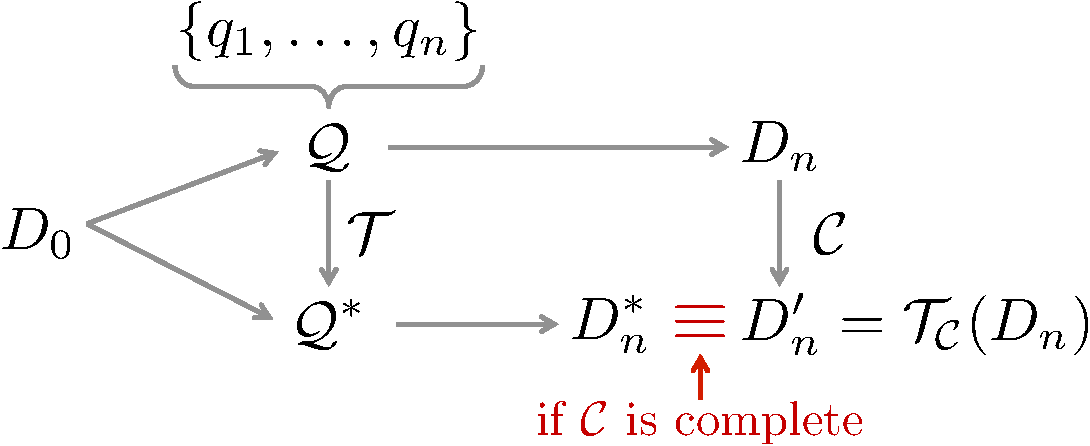
\includegraphics[width = 0.75\columnwidth]{figures/probtransform}
% \caption{Graphical depiction of the diagnosis problem in our \sys framework.  $D_0$, $D_n$, $\mathcal{Q}$, and $\mathcal{C}$ are given, and \sys uses them to derive the log repair $\mathcal{Q}^*$.
% \alex{not sure if this figure is actually useful.}}
% \label{f:probtransform} 
% \end{figure}


% \deprecate{
% \subsection{Naive Formulation}
% 
% The most general version of the problem
% (depicted in Figure~\ref{f:probtransform}) is to find a sequence of
% transformations $T$ that insert, delete, and/or modify queries in $Q_{seq}$ 
% such that the resulting sequence, $Q'_{seq} = T(Q_{seq})$, resolves the user's complaint set. 
% 
% However this problem is ill-defined because there exist an unbounded set of transformations that
% can resolve the user's complaint set.  A naive solution is to append to the query log a statement
% that deletes all the records in the database, followed by a query that insert all of the correct records.
% Unfortunately this naive solution does not help explain the complaints in any way!
% 
% \subsection{Constraints}
% 
% For this reason, we constrain the set of possible transformations $\mathcal{T}$ to the following:
% 
% \begin{itemize}
% \item delete query
% \item modify insert statement constants
% \item modify constants in WHERE clause
% \end{itemize}
% 
% Our transformations don't include adding new queries, synthesizing arbitrary queries, or modifying the
% number of clauses in a WHERE condition.  We apply these restrictions because we believe it is more likely
% for the user to mis-type a constant value as opposed to having an error in the query structure.
% 
% Futhermore we define a distance metric between two query logs in order to evaluate
% the qulatiy of a transformation.
% \xxx{define $\mathcal{T}$ here.}
% 
% 
% 
% \subsection{Problem Statements}
% 
% In this paper, we present three variants of this problem.
% 
% \begin{problem}[Prob-Complete]\label{prob:complete}
% Given $C = P_{D_n, D^*_n}$, $Q_{seq}$, and the sequence of database states $D_0,\ldots,D_n$, 
% identify a sequence of transformations $T$ such that:
% \begin{itemize}
% \item $T(Q_{seq})(D_0) = C(D_n)$
% \item $|T| = 1$
% \item $T$ metric is minimized
% \end{itemize}
% \end{problem}
% 
% This variation of the problme relaxes the constraint that the complaint set must be complete, and allows
% for both false positives as well as false negatives.  The goal is the same, however the constraints are relaxed:
% 
% \begin{problem}[Prob-Incomplete]\label{prob:incomplete}
% Given $C$ where $acc_C < 1$, $Q_{seq}$, and the sequence of database states $D_0,\ldots,D_n$, 
% identify a sequence of transformations $T$ such that:
% \begin{itemize}
% \item $T(Q_{seq})(D_0) = D^*_n$
% \item $T$ metric is minimized.
% \item $|T| = 1$
% \end{itemize}
% \end{problem}
% 
% Finally, we extend the problem to allow transformations with one or more operations.
% 
% \begin{problem}[Prob-MultiQ]\label{prob:multi}
% Given $C$ where $acc_C < 1$, $Q_{seq}$, and the sequence of database states $D_0,\ldots,D_n$, 
% identify a sequence of transformations $T$ such that:
% \begin{itemize}
% \item $T(Q_{seq})(D_0) = D^*_n$
% \item $T$ metric is minimized.
% \end{itemize}
% \end{problem}
% 
% 
% 
% 
% \subsection{A Naive Approach}
% 
% \begin{itemize}
% \item roll back complaints to penultimate state using algebraic expressions 
% \item perturb each expression in query until the query result matches correct state
% \item if an expression cannot be found, iterate
% \end{itemize}
% 
% 
% Not clear how to roll back complaints
% 
% Ways to perturb query expressions is unbounded
% 
% }
%!TEX root = ../main.tex

\section{A MILP-based Solution}
\label{sec:sol}

In this section, we introduce an exhaustive solver-based approach to 
resolve the errors reflected in the complaint set.
This approach constructs a mixed-integer linear 
programming (MILP) problem~\cite{milp} by linearizing and parameterizing the 
corrupted query log over the tuples in the database. 
Briefly, an MILP is a linear program~\cite{} where only a subset of the undetermined variables
are required to be integers, while the rest are real valued.

Our general strategy is to model each query as a linear equation 
that computes the output tuple values from the inputs and to transform the
equation into a set of of linear constraints.   
In addition, the constant values in the queries are parameterized
into a set of undetermined variables, while the database state is encoded 
as constraints on the initial and final tuple values.
Finally, the undetermined variables are used to construct an objective function
that prefers value assignments that minimze both the amount that the queries change and
the number of non-complaint tuples that are affected. \alex{I was under the impression that we stick to using the non-complaint tuples as constraints.}

The rest of this section will first describe the process of linearizing a single query
and translating it into a set of constraints.  We then extend the process to the entire
query log and finally define the objective function.
Subsequent sections introduce optimizations that both
improve the speed and quality of the results, as well as harness the trade-off between the two. 


% \xlw{Essentially, 
% we convert the updating process of the query log into a set of 
% constraints, transform values in queries (in the query log)
% as undetermined variables, and 
% using these values to form the objective function. Thus, the problem of 
% deriving a log repair is converted into a mixed-integer linear 
% programming (MILP) optimization problem. }\\
% {\xlw{need to introduce MILP problems a little bit here, so readers know what undetermined
% variables are and why things need to be linearized}}






\subsection{Encoding a Single Query}%Linearizing \& Parameterizing Single Query}
\label{sec:linearize}

\if{0}
  We model a query $q_i$ as a conditional function $f_{q_i}(t)$ that takes as input a tuple $t$
  and returns its next state $t'$.  $f_{q_i}$ is applied to each 
  tuple $t \in \mathcal{D}_{i-1} \cup \{\bcancel{t}\}$ in the input relation along with a special
  non-existant tuple $\bcancel{t}$. \ewu{maybe fold this into the data model.}
  By treating the query as a function, we are able to encode its effects into a set
  of linear inequality constraints.  We call this process the linearization and 
  parameterization of a query.

  \begin{definition} [Conditional Function]
  \label{def:cond}
    The conditional function for query $q$ is:
    \[
      f_{q_i}(t)= 
      \begin{cases}
      f_{q_i.\mu} (t) ,& \text{if } f_{q_i.\sigma} (t)\\
      t,              & \text{otherwise}
      \end{cases}
  \]
  where the \textit{update function} $f_{q_i.\mu}$ models a set of \textit{update equation(s)};
  and the \textit{condition function} $f_{q_i.\sigma}$ models a set of \textit{logical expression(s)} in 
  disjunctive or conjunctive form.
  \end{definition} 


  % We linearize and parameterize a query $q$ by considering its effects on the 
  % targeted table $R(A_1, ..., A_m)$: we treat the query $q$ as a 
  % conditional function over each tuple $t\in R$ and convert the effects of $q$ 
  % over $t$ into a set of linear inequality constraints. 
  % \subsubsection{Query as a Conditional Function}
  % The effect of query $q$ over a tuple $t$ can be expressed in a conditional
  % function $f_q(t)$ as the following:

  Conditional functions can describe the common classes of update queries:
  \begin{enumerate}
  \item \texttt{UPDATE}: $f_{q_i.\mu}(t)$, $f_{q_i.\sigma}(t)$ model the \texttt{SET}
        and \texttt{WHERE} clauses.  For example, $f_{q_i.\mu}(<t.a, t.b>) = <t.a + 1, 2>$ and
        $f_{q_i.\sigma}(t) = (t.a > 20)$ corresponds to the query 
        \texttt{UPDATE D SET a = a + 1, b = 2 WHERE a > 20}.

  \item \texttt{INSERT}: $f_{q_i.\mu}(t)$ returns the inserted tuple, while 
        $f_{q_i.\sigma}(t) = (t = \bcancel{t})$ evaluates to true when it is executed over
        the special nonexistant tuple.
        %is a boolean variable reflects 
        %the existence of tuple $t$; $\vee_{t\in R} f_{q.\sigma}(t)$ represents 
        %the existence of this insert query.  

  \item \texttt{DELETE}: $f_{q_i.\mu}(t) = \bcancel{t}$ returns a nonexistant tuple whenever
        the predicate encoded in $f_{q_i.\sigma}(t)$ evaluates to true.
        For example, the query \texttt{DELETE FROM T WHERE a < 20} represents 
        $f_{q_i.\sigma}(t) = (t.a < 20)$.
        
        % the deleted values for 
        % each attribute and $f_{q.\sigma}(t)$ reflects the expressions in where clause 
        % (similar to $f_{q.\sigma}(t)$ in \texttt{UPDATE} query).
  \end{enumerate}

  Finally, we parameterize $q_i$ by replacing all numeric constants in the
  conditional function with undetermined variables.   Consider the conditional
  function for \texttt{UPDATE} above: the constants $1$, $2$ in $f_{q_i.\mu}$
  as well as $20$ in $f_{q_i.\sigma}$ will be transformed into undetermined
  variables \texttt{v1, v2, v3} that are solved by the MILP solver.

  % We parameterize query $q$ by replacing all numeric values in the above conditional 
  % function into undetermined variables (Example~\ref{ex:parameterize}).
  % \begin{example}\label{ex:parameterize}
  % Consider a \texttt{UPDATE} query $q$:
  % \texttt{UPDATE R SET A$_1$ = 3 WHERE A$_2$ $\leq$ 10},
  % the conditional function of this query is: 
  % \[
  %     f_q(t)= 
  % \begin{cases}
  %     f_{q.\mu}(t) = \{t.A_1 = 3\} ,& \text{if } f_{q.\sigma}(t) = \wedge\{t.A_2 \leq 10\}\\
  %     t,              & \text{otherwise}
  % \end{cases}
  % \]
  % The numeric variables in query $q$ including \texttt{3} in $f_{q.\mu}(t)$ and \texttt{10}
  % in $f_{q.\sigma}(t)$. Thus, we parameterize query $q$ by replacing the value \texttt{3, 10}
  % by two undetermined variables \texttt{var1, var2}. 
  % \end{example} 
\fi



% \subsubsection{Constructing Linear Inequality Constraints}

MILP problems require that the constraints are expressed as a set of linear
(in)equality constraints, thus our task is to linearize the parameterized
conditional function.   We will individually describe this linearization process 
to represent the value of a single attribute $A_j$ and a single tuple $t$ for 
\texttt{UPDATE}, \texttt{INSERT}, and \texttt{DELETE} queries; 
extending the process to the rest of the attributes is a straighforward exercise.
% Now that we have modeled $q_i$ as a parameterized conditional function, 
% we must linearize $f_{q_i}$ into a set of linear (in)equality constraints
% for the MILP problem.



\stitle{\textbf{UPDATE:} }
Recall from Section~\ref{sec:models} that query $q_i$ can be modeled as
the combination of a modifying function $\mu_{q_i}(t)$ and conditional function $\sigma_{q_i}(t)$.
We can re-express the value of attribute $A_j$ in the updated tuple $t'$ as the following equation:
{\scriptsize
\begin{eqnarray}
\label{eq:linearization}
t'.A_j = x_{q_i, t}\otimes \mu_{q_i}(t).A_j + (1-x_{q_i, t})\otimes t.A_j 
\end{eqnarray} 
}


\noindent Where the binary variable $x$ is introduced to represent the output of 
the conditional function:
{\scriptsize
\begin{eqnarray}
\label{eq:x}
x_{q_i, t} = \sigma_{q_i}(t)
\end{eqnarray}
}
We then introduce two variables $u.A_j$ and $v.A_j$ to represent 
the respective components in Equation~\ref{eq:linearization}, where
$M$ representes the upper bound of $t.A_j$'s domain:
{\scriptsize 
\begin{eqnarray}
\label{eq:uv}
u.A_j &\leq & \mu_{q_i}(t).A_j \nonumber\\
u.A_j &\leq & x_{q_i, t}M \nonumber\\ 
u.A_j &\geq & \mu_{q_i}(t).A_j - (1-x_{q_i, t})M \nonumber \\\nonumber \\
v.A_j &\leq & t.A_j \nonumber\\
v.A_j &\leq & (1-x_{q_i, t})M \nonumber\\
v.A_j &\geq & t.A_j - x_{q_i, t}M
\end{eqnarray}
}
The first set of conditions forces $u.A_j = \mu_{q_i}(t).A_j$ if $x_{q_i, t}=1$, and $0$ otherwise.  
The second set forces $v.A_j = t.A_j$ if $x_{q_i, t}=0$, and $0$ otherwise.  
Now, Equation~\ref{eq:linearization} is simply a linear equation:
{\scriptsize\begin{eqnarray}
\label{eq:tnew}
t.A_j' = u.A_j + v.A_j
\end{eqnarray}}



\stitle{\textbf{INSERT:}}
An insert query adds a new tuple $t_{new}$ to the database.  If the query were 
corrupted, then the inserted values may need to be repaired.  Thus, we allocate
an undetermined variable for each of the inserted tuple's attributes:
{\scriptsize
\begin{eqnarray}
\label{eq:insert}
t'.A_j = x \otimes t_{new}.A_j + (1-x) \otimes v.A_j 
\end{eqnarray}
}
\noindent Where $x$ is an undetermined binary variable that represents whether
the query is incorrect.  If it is, then it takes the value of an undetermined real 
variable $v.A_j$.


\stitle{\textbf{DELETE:}}
A delete query removes a set of tuples from the database.  
Since the MILP problem doesn't have a way to express a non-existant value, 
we encode a deleted tuple by setting its attributes to a value
outside of the attribute domain $M^+$.  In this way, subsequent conditional functions
on the attribute will return false, so it will not have an effect on subsequent queries encoded
in the MILP problem:
{\scriptsize
\begin{eqnarray}
\label{eq:delete}
t'.A_j &=& x_{q_i, t} \otimes M^+ + (1-x_{q_i, t}) \otimes t.A_j \nonumber \\
x &=& \sigma_{q_i}(t)
\end{eqnarray}
}


\stitle{\textbf{Putting it All Together:}}

% )(\ref{eq:uv})(\ref{eq:tnew})(\ref{eq:insert})(
The above constraints (\ref{eq:x}--\ref{eq:delete})
form the main structure of MILP subproblem for a single attribute $A_j$ of a single tuple $t$.
In this incomplete form, all of the variables including the binary variables $x_{q_i, t}$,
the real-valued attribute values (e.g., $u.A_j$),
and the real-valued constants in $\mu_{q_i}$ and $\sigma_{q_i}$ are all undetermined
and need to be assigned values by a MILP solver.  
To linearize $q_i$, we can simply apply the same procedure for each attribute in the 
query and every tuple in the database.
We describe the above linearization process as the function 
$Linearize(q, t)$, which takes a query $q$ and tuple $t$ as input.

The final step is to assign concrete values to the starting and ending attribute values 
$t.A_j$ and $t'.A_j$ based on the starting database state $D_{i-1}$ and the ending database 
state that has been transformed by $\mathcal{C}$, $D'_i$.
In this way, only the query parameters and the binary $x_{q_i, t}$ variables are undetermined;
a solution to the MILP formulation will assign values to those undetermined variables
such that the resulting query fixes the complaints correctly.

The next subsection will describe how to extend the above encoding procedure to the 
entire query log, and how to incorporate an objective function that encourages solutions
that minimize the amount of changes to the query log.  







\subsection{Encoding and Repairing the Query Log}
\label{sec:milp}

We are now ready to describe the procedure (Algorithm~\ref{alg:basic}) to encode 
the full query log into a MILP problem, and solve the MILP problem to derive $\mathcal{Q}^*$.
The algorithm takes as input the query log $\mathcal{Q}$, 
the initial and final (dirty) database states 
$\mathcal{D}_{0, n}$, and the complaint set $\mathcal{C}$, and outputs a fixed query 
log $\mathcal{Q}^*$.  

We first call \textit{Linearize} on each tuple in $\mathcal{D}_0$ and each query in $\mathcal{Q}$, 
and add the result to a set of constraints \textit{milp\_cons}.
Similar to the single-query procedure, \textit{AssignVals} additionally 
adds constraints to fix the values of the inputs to $q_0$ and 
the outputs of $q_n$ to their respective values in
$\mathcal{D}_0$ and $\mathcal{C}(\mathcal{D}_n)$.
Next, we add constraints to take into account the fact that the output of 
query $q_i$ is the input of $q_{i+1}$ (\textit{ConnectQueries}).
This function simply equates $t'$ from the linearized result for $q_i$ to the $t$ input 
for the linearized result of $q_{i+1}$.

Finally, we use the undetermined variables in \textit{milp\_cons}, along with $\mathcal{Q}$,
to encode the distance function $d$ described in Section~\ref{def:obj} 
into the MILP objective function, and submit it to a MILP solver.
\textit{ConvertQLog} replaces the constants in the query log with the 
assigned values for the undetermined variables in the solution, and constructs
the fixed query log $\mathcal{Q}^*$.
\ewu{explicitly mention each function in algorithm.}



% Using the linearization method in Section~\ref{sec:linearize}, we can further
% linearize the entire query log by converting every tuples in the table $R$. 
% During the linearization, we further parameterize each
% query in the query log $\mathcal{Q}$ in order by derive the log repair. 
% The linearized and parameterized query log
% should start from and end at clean database states.
% To achieve this, we add constraints by assigning the true initial and end database 
% states' values (based on complaints) to the corresponding variables. 
% Following the above steps (Algorithm~\ref{alg:basic}), we convert the 
% query log into a collection of constraints with newly introduced variables. 
% Some of these variables are introduced to linearize the query log 
% and the rest usually represent the numeric values in the query log
% during the paramerization process. 
% The latter set of variables often involved in the objective function 
% according to the pre-defined distance function $d$ 
% (as described in Definition~\ref{def:problem}). 


\begin{algorithm}[htbp]
\caption{$QueryFix_{exh}$ based on MILP formulation.}
\label{alg:basic}
\scriptsize
\begin{algorithmic}[1]
\REQUIRE {$\mathcal{Q}, D_0, D_n, \mathcal{C}$}
%\ENSURE {$\mathcal{Q^*}$}
\STATE $milp\_cons \leftarrow \emptyset$
\FOR {each $t$ in $R$}
\FOR {each $q$ in $\mathcal{Q}$}
\STATE $milp\_cons \leftarrow milp\_cons \cup Linearize(q, t)$
\ENDFOR
\STATE $milp\_cons \leftarrow milp\_cons \cup AssignVals(D_0.t, D_n.t, \mathcal{C})$
\FOR {each $i$ in $\{0,\ldots,N-1\}$}
\STATE $milp\_cons \leftarrow milp\_cons \cup ConnectQueries(q_i, q_{i+1})$
\ENDFOR
\ENDFOR 
\STATE $milp\_obj \leftarrow EncodeObjective(milp\_cons, \mathcal{Q})$
\STATE $solved\_vals \leftarrow MILPSolver(milp\_cons, milp\_obj)$
\STATE $\mathcal{Q}^* \leftarrow ConvertQLog(Q, solved\_vals)$
\STATE Return $\mathcal{Q}^*$
\end{algorithmic}
\end{algorithm}

% By constructing linear (in)equality constraints and
% defining a objective function, we convert the problem into
%  a mixed-integer linear programming (MILP) problem that can be 
%  solved by MILP solvers. By solving this MILP problem, we collect the
% corrections for the parameterized variables and form the log repair. 

% describe how to linearize the whole querylog with provided
% database states info. 


















%!TEX root = ../main.tex

\section{Optimizing the Basic Approach}
\label{sec:opt}

A large drawback of our basic MILP transformation (Section~\ref{sec:sol}) is
that it exhaustively encodes the combination of all tuples in the database and all queries
in the query log.  In this approach, the number of constraints (as well as undetermined variables) 
grows quadratically with respect to the database and the query log.
Figure~\ref{fig:querysize_vs_time} shows a simple scalability experiment, where we generated increasingly 
larger query logs for a database of $1000$ tuples, encoded the problem using \naive (red bars), 
and solved the problem using a MILP-solver (CPLEX in our experiments).
We find that the solver time increases exponentially as the number of encoded queries increases --
at a log size of $80$, the solver failed to produce an answer within $1000$ seconds --
due to the exponential increase in the number of possible states for the increasing number of undetermined variables.
In contrast, the blue bar illustrates the near-constant performance of a similarly encoded but optimized MILP problem. 
% {\it only parameterizes the constants of the oldest query in the log}.
Although the empirical solver performance varies widely depending on the specific problem, 
this experiment illustrates the limitations of the na\"ive approach.

\begin{figure}[h]
    \centering
    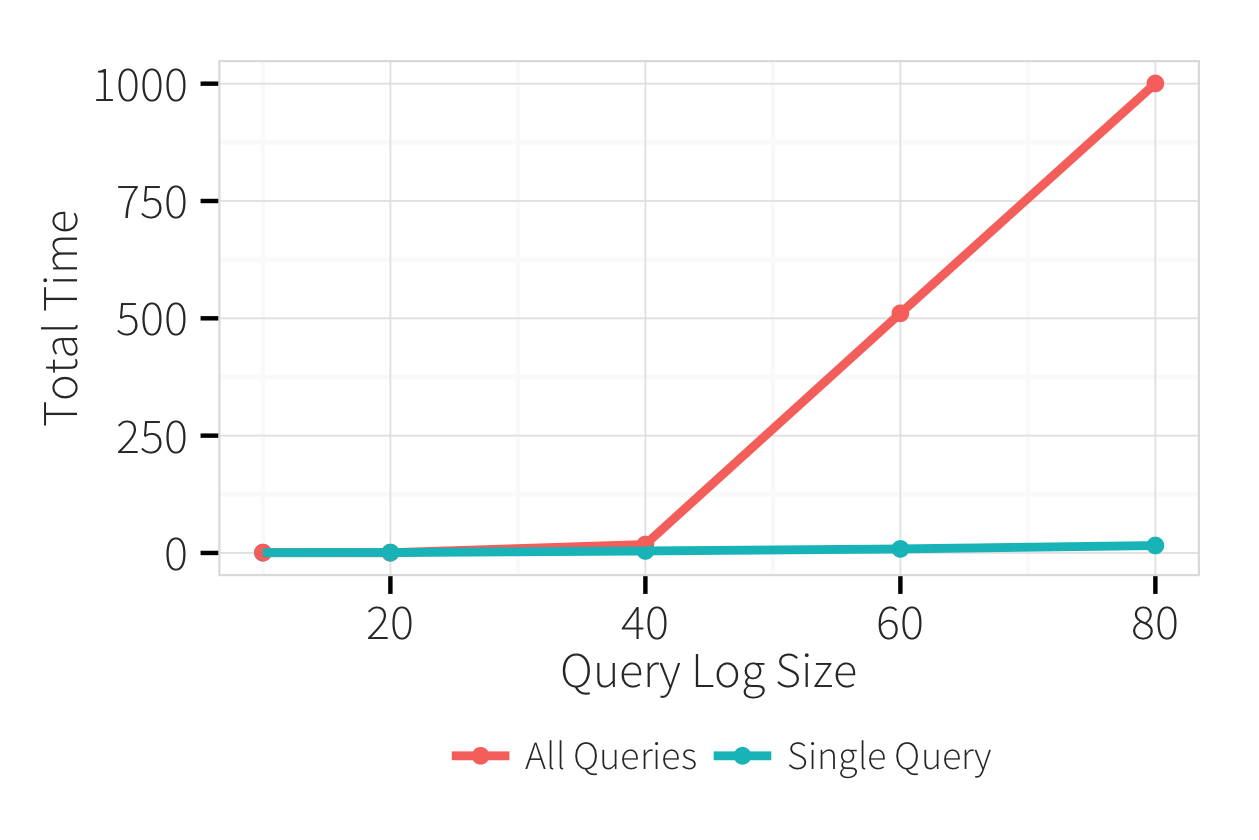
\includegraphics[width=0.35\textwidth]{figures/qsize_time_badscale}
    \vspace*{-0.1in}
    \caption{Log size vs. execution time on synthetic setup. }
    \label{fig:querysize_vs_time}
\end{figure}

To resolve this limitation, we explored three classes of \emph{slicing} optimizations that seek to
reduce the number of tuples, queries, and attributes that are encoded in the MILP problem.
In addition, we propose an incremental algorithm that exploits the single bar performance observed
in the above scalability experiment, which both improves the scalability and the repair latency
when the corrupted query is recent.  




% In the previous section, we introduce the basic approach to derive
% the log repair by incorporating information from every query
% and every tuple into a single MILP problem. However, oftentimes, 
% this basic approach end up with 
% a huge problem as the query log size and table size increase. 
% In Figure~\ref{fig:querysize_vs_time}, 
% we observe that the total solver (IBM CPLEX) solving time 
% grows exponentially and 
% unpredictably as the query 
% log size or the table size increases. As a result, the basic approach does not scale over 
% large problems (large query log size and large table size).


\if{0}
linearize whole query log, so cost of adding an additional tuple is very high.
second iteration generally takes ~1 - 10%
for large databases knn cost is pretty high: ~

if the solver returns, it is always a super set of the clean range

only tuples modified by the fixed queries
- tuples already in the complaints (correct)
- not in complaints, but any of the originial queries modified it
- not in complaints, but no original queries modified it
\fi



\subsection{Reducing Tuples (Tuple Slicing)}
\label{sec:opt:tbsize}
\begin{figure}[t]
    \centering
    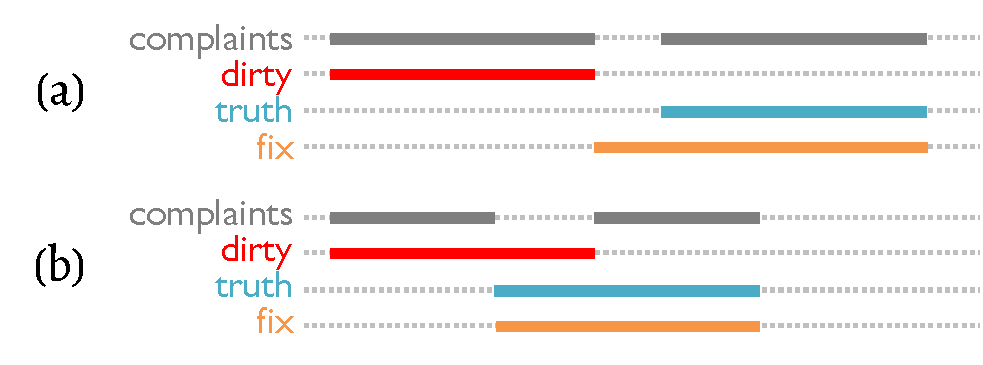
\includegraphics[width=0.35\textwidth]{figures/2nditerationgroups}
    \vspace*{-.2in}
    \caption{Graphical depiction of succeed\&failed repairs. Each solid and empty circle represents a complaint and non-complaint tuple.
Each thick line represents the interval of query $q$'s range predicate: 
dirty is the incorrect interval in the corrupted query,
truth is the correct interval in the true query, 
and repair is the interval returned by the solver.}
    \label{fig:groups}
    \vspace*{-.2in}
\end{figure}

% \ewu{Assume reader is clear that we are only repairing WHERE clause range predicates}
Our first optimization, \emph{tuple slicing}, applies a two steps process to reduce the 
problem size without sacrificing accuracy: it
first aggressively reduces
the problem size by only encoding tuples in the complaint set and then refines the log repair 
through a separate but much smaller MILP problem. 
\noindent\textit{Step 1 (Generate Initial Repair):} \\
The first step of  \emph{tuple slicing} 
aggressively reduces the problem size by only encoding those 
tuples in the complaint set $\mathcal{C}$ (Algorithm~\ref{alg:basic} line $2$
is replaced with \texttt{for each t in $\mathcal{C}$}). 
Each tuple necessitates
the linearization of the entire query log, thus, only encoding the complaint tuples minimizes the 
size of the problem with respect to the relevant tuples. This aggressive optimization is guaranteed to resolve $\mathcal{C}$ , thus it sometimes helps
fixing query logs magnitude faster without hurting the accuracy: For example, in Figure~\ref{fig:groups}(a), the dirty and truth intervals overlap, thus the non-complaint tuples 
within the overlapping region are correctly modified by the dirty interval. 
(Recall that we do not have access to the truth interval, and our goal is to reproduce the 
truth interval given $\mathcal{C}$ (solid circles) and the corrupted query.) 
In this case, the proposed repair correctly contains the non-complaint tuples and the algorithm is successful.\\
\indent However, sometimes the problem may overfit 
and not generalize to the entire database.
Specifically, there are problem settings where the repaired range predicate in a query's \texttt{WHERE} clause is a superset of the true range predicate, and introduces new errors by affecting tuples not originally part of  the complaint set. 
Figure~\ref{fig:groups}(b) highlights such a case where this aggressive approach generalized incorrectly.
The dirty and clean intervals are non-overlapping, so the non-complaint tuple shown is not modified by $q$ (otherwise it would be a complaint!). This tuple is incorrectly included in the repaired interval, \emph{because the MILP formulation does not constrain its value}.

\indent Note that in both of these cases, the objective function will ensure that the repair
does not over-generalize the upper bound towards the right because that strictly increases the objective function.
On the other hand, over-generalizing the lower bound towards the dirty interval
is expected because it decreases the Manhattan distance between the repaired and corrupted lower bounds,
which are parameters in the objective function. Therefore, to perform tuple slicing successfully, we need to reduce the repaired interval and exclude those non-complaint tuples in case (b).  

\noindent\textit{Step 2 (Refine Initial Repair):}
Although there are many possible mechanisms to refine the initial repair (e.g., incrementally shrinking
the repaired interval until the non-complaint tuples are all excluded), 
the straightforward approaches are not effective when multiple corrupt 
queries have been repaired because they don't take the query interactions into account.

Instead, we solve this using a second, significantly smaller, MILP problem.   
Let $\mathcal{Q}^*_{sub}$ be the set of repaired queries from the  initial MILP formulation with tuple slicing.
We identify the set of non-complaint tuples $\mathcal{NC}$ that are now included in a repaired \texttt{WHERE} clause predicate, as in Figure~\ref{fig:groups}(b). We construct a new MILP by linearizing the log over $\mathcal{C}^+ = \mathcal{C} \cup \mathcal{NC}$, but we set the values of all variables not in $\mathcal{Q}^*_{sub}$ to their corresponding assignment from the initial MILP solution
This ensures that only repaired query parameters can
be perturbed, which vastly reduces the number of undetermined variables in the problem.
Second, we modify the objective function to only penalize the number of non-complaint tuples 
$t \in \mathcal{C}^+$ that are matched by the queries in $q \in \mathcal{Q}^*_{sub}$.
These selections are represented by the binary variable $x_{q, t}$, thus the updated objective function
is $\sum_{q \in \mathcal{Q}^*_{sub}} \sum_{t \in \mathcal{NC}} x_{q,t}$.

% % \alex{I don't think this is true; it doesn't interfere with incomplete complaints, but it is not a mechanism to solve them.}
% We use this same mechanism to address incomplete complaint sets.
In our experiments, we find that this second MILP iteration adds
minimal overhead ($0.1-0.5\%$) with respect to the initial MILP
problem, making \tslice and effective method to improve the performance of the basic approach, without compromising accuracy.

% \ewu{Need to clarify that the solver is a black box, who knows what goes on there.  Maybe where we introduce MILP-solvers}
% \xlw{The number of noncomplaints differs case by case. }


% Although the query log is linearized in the same fashion as the above tuple slicing optimization,
% we additionally include the non-complaint tuples that are selected by the repaired queries in the problem.
% We then set the value of all of the variables to the results of the 
% We then updae the objective function so
% 
% we dramatically reduce the number of undetermined variables and use a different objective function.
% We fix all of the undetermined variables e
% 
% The simple approach 
% Let $\mathcal{Q}^*_{sub}$ be the set of repaired queries.
% We first construct a set of constraints by linearizing the queries in the query log
% between the least and most recent queries in $\mathcal{Q}^*_{sub}$ with respect to $\mathcal{C}$.
% The key difference is that we repair all of the undetermined variables for $x$ in Equation~\ref{}
% based on the solutions to the first MILP problem.  
% In addition, we call $Linearize$ for each non-complaint tuple in the repaired interval.
% The objective function is to minimize the sum of the undetermined $x$ variables in the encoded
% problem.
% 

% fix is always the smallest possible, so it can only require a sceond iteration if the dirty and clean
% ranges don't overlap at all.  
% 
% The basic solution, which suggests to linearize every tuple in the database into the MILP problem,
% has two major disadvantages: 1. the system may end up with a large MILP problem that requires 
% the solver to run forever to solve; 2. we can only linearize the every tuple
% when the complaint set is complete, which is often hard to guarantee. Thus, in the first 
% optimization, we propose a two-iteration approach handles both of these two problems 
% by linearizing tuples in the complaint set in
% the 1st iteration and refining the log repair in the 2nd iteration. \\
% \subsubsection{1st iteration}
% We use tuples in the complaints $\mathcal{C}$ to construct the MILP problem and derive a 
% inaccurate log repair $\mathcal{Q}^*$\xlw {we need to find a term for this}. This inaccurate 
% log repair resolves tuples in the complaints $\mathcal{C}$, but, at the same time, 
% introduces noises by over correcting tuples that are not involved in the MILP problem. 
% As shown in Example~\ref{ex:2nditer}, by resolving tuples in complaints $\mathcal{C}$, 
% the system derives a log repair that introduces other errors. 
% \begin{example}\label{ex:2nditer}
% Including tuples in the complaints $\mathcal{C}$ to solve problem in Example~\ref{ex:taxes2} 
% and using Euclidean distance of variables in the query as the objective function, the system 
% derives a log repair $\mathcal{Q}^*$ with $q_1^*=$ \texttt{\small UPDATE Taxes SET rate = 30}
% \texttt{\small WHERE income >= \color{red}{9500.0001} \color{black}{and income <=} \color{red}{90000}}. 
% This log repair resolve tuples in the complaints. However, the fixed query $q_1$ has a much wider range 
% and it it incorrectly modifies tuples that are not in the complaint, e.g., tuple $t_4$.
% \end{example}
% \ewu{why would this happen if we encoded all the tuples?  Doesn't the objective penalize this case?}
% 
% 
% To avoid introducing such noises, we introduce the 
% 2nd iteration which targets on refining the log repair derived in 
% the 1st iteration. 
% \subsubsection{2nd iteration}
% The goal for 2nd iteration is to optimize the impact of the log repair (tuples
% modified by $\mathcal{Q}$). 
% Let $\mathcal{Q}^*_{sub} = \mathcal{Q}^*-\mathcal{Q}$ as 
% queries modified in the log repair, in the 2nd iteration, we 
% construct a separate MILP problem by linearizing 
%  queries between the first and the last query in
% $\mathcal{Q}^*_{sub}$, parameterizing variables in 
% the where clause for queries in $\mathcal{Q}^*_{sub}$,
% and maximizing the log repair impact score. 
% 
% 
% We define the impact score by dividing the 
% impacted tuples $T$ into three groups and defining the 
% impact score accordingly. \xlw {we need to fix these terms}. 
% 
% \smallskip
% 
% \noindent\textbf{Group 1}: tuples in the complaints $\mathcal{C}$. Impact of 
% $\mathcal{Q}^*$ on this group
% are guaranteed as correct. \textbf{Rule:} 
% strictly satisfy, including these tuples as 
% constraints in the 2nd iteration MILP problem. 
% 
% \smallskip
% 
% \noindent\textbf{Group 2:} tuples not in $\mathcal{C}$, but also modified 
% by the original query log $\mathcal{Q}$. Impact of $\mathcal{Q}^*$ 
% on the group 2 are likely to
% be correct. \textbf{Rule:} adding these tuples into the 
% rewarded tuple set $T_{reward}$. 
% \ewu{what does "modified by the original query log Q mean?}
% 
% \smallskip
% 
% \noindent\textbf{Group 3:} tuples not in $\mathcal{C}$ and not modified 
% by the original query log $\mathcal{Q}$. Impact of 
% $\mathcal{Q}^*$ on the last group should penalized, thus 
% we put them into $T_{penalize}$ (\textbf{Rule}).
% 
% \smallskip
% 
% The impact score, which is also the objective function for
% the MILP problem, is $T_{reward} - T_{penalize}$. \ewu{what exactly is this objective function?  the number of tuples modified?}We further 
% optimize the 2nd iteration to reduce the size of $T$ 
% by searching for K-nearest-neighbors
% of tuples in complaints $\mathcal{C}$. 
% There are multiple benefits for the two-iteration approach:
% \begin{itemize}
% \item It minimizes the size of MILP problem in the 1st iteration. 
% \item It refines the log repair while avoid over correcting tuples not in 
% the complaints $\mathcal{C}$. 
% \item It pptimizes the impacted tuples efficiently by controlling the queries 
% and number of impacted tuples
% involved in the 2nd MILP problem.
% \item In addition, it handles cases when we don't have complete complaints
% $\mathcal{C}$ (false negatives). 
% \end{itemize}




\if{0}
  \subsubsection{A Naive but Flawed approach}
  \ewu{Better explained as: CPLEX searches through an exponential space of all possible combinations of MILP variables.  In a chunked approach, the solution of each chunk is one out of a potentially arbitrary number of possible solutions, thus it is easy to pick an incorrect one}
  A natural idea to optimize the basic approach is 
  to \textbf{chunk the query log} into
  smaller, fixed size pieces and then solve each piece at a time: starting
  from the most recent piece, the system linearizes and parameterizes queries 
  in the current piece and derives a corresponding log repair; 
  it then examines the other pieces iteratively
  in the same way. Since complaints only provides
  true values for the most recent database state, in order to avoid 
  linearizing additional queries, 
  we need to know \textbf{rollback} the true values of tuples 
  until the last query in each query log piece. \\
  However, rollback the database is non-easy. An ideal, precise rollback
  algorithm would generate a set of valid ranges for each attribute of a tuple. 
  But the size of valid ranges also grows exponentially with the number queries
  we want to rollback, which, in turn, could not improve the system performance. 
  On the other hand, an approximate, imprecise 
  rollback algorithm would either make the rest of the problems
  infeasible to solve (only maintain fixed number of valid ranges) 
  or result in deriving 
  incorrect log repairs (maintain the lower 
  bound and upper bound among all valid ranges).
    

  In order to improve the system performance without losing accuracy, we propose
  the following two optimizations: query-slicing optimization 
  based on provenance over queries and
  attribute-slicing optimization based on provenance over 
  attributes. 
\fi





\subsection{Reducing Queries (Query-Slicing)}
\label{sec:opt:query}


In practice, many of the queries in the query log could not have affected the \emph{complaint attributes} (defined below). For example, if $q_{N-1}$ and $q_{N}$ 
only read and wrote attribute $A_1$, then they could not have contributed to an error in $A_2$.  
However, if $q_{N}$  wrote $A_2$, then either or both queries may have caused the error. 
In short, if we model a query as a set of attribute read and write operations, those that form a 
causal read-write chain to the \emph{complaint attributes} must be linearized, whereas others can be ignored.  This is the foundation of our \emph{query-slicing} optimization.

% The exhaustive parameterization of all queries in the query log, as described
% in the basic approach, is typically unnecessary because many queries in the log
% could not have affected the tuple attribute values in the complaint set.
% To avoid such redundant computation, \textit{query-slicing} 
% removes \texttt{UPDATE} queries whose \texttt{SET} clauses did not modify 
% attributes that could possibly have affected the {\it complaint attributes} 
% specified in the complaint set.

\begin{definition} [Complaint Attributes $\mathcal{A}(\mathcal{C})$]
	The set of attributes identified as incorrect in the complaint set.
	\[\mathcal{A}(\mathcal{C}) = \{A_i | t.A_i \neq t^*.A_i, c(t,t^*) \in \mathcal{C}\}\]
\end{definition} 


\begin{definition}[Query dependency \& impact]
    Query $q_i$ has \textbf{direct-impact}, $\mathcal{I}(q_i)$, which is
    the set of attributes updated in its modifier function $\mu_{q_i}$
    (e.g., \texttt{SET} clause). Its \textbf{dependency},
    $\mathcal{P}(q_i)$, is the set of attributes involved in its
    condition function $\sigma_{q_i}$.
    
    We derive the \textbf{full-impact}, $\mathcal{F}(q_i)$, of a query $q_i$ by propagating its direct impact through subsequent queries in the log (Algorithm~\ref{alg:fullimpact}):
    \[
    \mathcal{F}(q_i)=\mathcal{I}(q_i)\bigcup_{\substack{j=i+1\\ \mathcal{F}(q_i)\cap \mathcal{P}(q_j) \neq \emptyset}}^n \mathcal{F}(q_j)
    \]
  % \begin{enumerate}
  %   \item The \textbf{dependency}, $\mathcal{P}(q)$, of a query $q$
  %   is the set of attributes involved in the condition function $\sigma_q$.
  %   %\[\mathcal{P}(q) = \Pi_{f_{q}.\sigma}(R)\]
  %   \item The \textbf{direct-impact} of query $q$, 
  %   $\mathcal{I}(q)$, is the set of attributes 
  %   updated in the modifier function $\mu_q$ 
  %   (e.g., \texttt{SET} clause).
  %   %\[\mathcal{I}(q) = \Pi_{f_{q}.\mu}(R)\]
  %   \item The \textbf{full-impact}
  %   of $q$, $\mathcal{F}(q)$, propagates $q$'s direct impact through
  %   the subsequent queries in the query log to collect {\it all} attributes
  %   that are affected by the changes caused by $q$'s update function.
  %   We describe its implications and computation below and in Algorithm~\ref{alg:fullimpact}.
  % \end{enumerate}
\end{definition}

% By comparing $\mathcal{F}(q)$ and $\mathcal{A}(C)$, we know whether
% or not corrupting query $q$'s parameters could possibly have caused the complaint
% set.  

% Algorithm~\ref{alg:fullimpact} describes how $\mathcal{F}(q_i)$ can be computed:
\begin{algorithm}[t]
\scriptsize
\caption{$FullImpact$ algorithm for finding $\mathcal{F}(q)$.}
\label{alg:fullimpact}
\begin{algorithmic}[2]
\REQUIRE {$\mathcal{Q}$, $q_i$}
% \ENSURE {$\mathcal{F}(\mathcal{Q})=\{\{\mathcal{F}(q_1)\}, ..., \{\mathcal{F}(q_n)\}\}$}
% \FOR {each $q_i$ in $q_n, ..., q_1$}
\STATE $\mathcal{F}(q_i) \leftarrow \mathcal{I}(q_i)$
\FOR {each $q_j$ in $q_{i+1}, ..., q_{n} \in \mathcal{Q}$}
\IF {$\mathcal{F}(q_i)\cap \mathcal{P}(q_j) \neq \emptyset$}
\STATE $\mathcal{F}(q_i) \leftarrow \mathcal{F}(q_i) \cup \mathcal{F}(q_j)$
\ENDIF
\ENDFOR
%\STATE $\mathcal{F}(\mathcal{Q}) \leftarrow \mathcal{F}(\mathcal{Q}) \cup {\red{\{\mathcal{F}(q_i)\}}}$
% \ENDFOR
\STATE Return $\mathcal{F}(q_i)$
\end{algorithmic}
\end{algorithm}
\vspace*{-.1in}

By computing the full-impact of $q$, we can determine the extent that it affects $\mathcal{C}$
based on its overlap with the complaint attributes.
Specifically, 
when $|\mathcal{F}(q) \cap \mathcal{A}(C)|=|\mathcal{A}(C)|$, $q$ may affect all complaint attributes and is a candidate for repair; 
when $0 < |\mathcal{F}(q) \cap \mathcal{A}(C)| < |\mathcal{A}(C)|$, 
$q$ contributed to a subset of the complaint attributes and is a candidate for repair;
when $|\mathcal{F}(q) \cap \mathcal{A}(C)|=0$, $q$ is irrelevant 
and can be ignored during the repair process.
We distinguish between the first and second conditions in the special case where we are repairing a \emph{single} 
corrupted query in the query log.  In this case, only queries in the first conditions are candidates for repair because 
the single query must have caused errors in all of the complaint attributes.  This enables \sys to scale significantly better
for this important problem setting. 
Finally, we use $Rel\mathcal{(Q)}$ to denote the set of relevant
queries that are candidates for repair. Our \emph{query slicing}
optimization, \qslice, linearizes only the queries in
$Rel\mathcal{(Q)}$, rather than the entire log, resulting in
smaller problems than \naive, without any loss of accuracy.

\subsection{Reducing Attributes (Attribute Slicing)}

In addition to removing irrelevant queries, we additionally avoid encoding irrelevant attributes.
Given $Rel\mathcal{(Q)}$, the relevant attributes can be defined as:
$Rel\mathcal{(A)} = \cup_{q_i \in Rel\mathcal{Q}} (\mathcal{F}(q_i)\cup \mathcal{P}(q_i))$
\aslice uses \emph{attribute slicing} to only encode constraints for attributes in $Rel\mathcal{(A)}$.
This type of slicing should be more effective for wide tables and query logs that focus a small subset of the attributes, such as TPC-C style transaction workloads. 
However, our experiments on synthetic workloads show that this optimization is not useful in many settings, and most improvements are achieved by slicing on the tuple and query dimensions.




\subsection{Single Query Incremental Repairs}\label{sec:incremental}

\begin{algorithm}[t]
\caption{\incremental algorithm. 
}
\scriptsize
\label{alg:incalg}
\begin{algorithmic}[2]
\REQUIRE {$Rel\mathcal{(Q)}, \mathcal{D}_j, \mathcal{D}_n, \mathcal{C}$}
\STATE Sort $Rel\mathcal{(Q)}$ from most to least recent
\FOR {each $q_i \in Rel\mathcal{(Q)}$}
  \STATE $\mathcal{Q}_{suffix}$ = $\{q_j | j \ge i \wedge q_j \in Rel\mathcal{(Q)}\}$
  \STATE $\mathcal{Q}^*$ $\leftarrow$ $QueryFix_{exh,param}(\mathcal{Q}_{suffix}, \mathcal{D}_j, \mathcal{D}_n, \mathcal{C}, q_i)$
  \IF {$\mathcal{Q}^* \neq \emptyset$}
    \STATE Return $q_i^* \in \mathcal{Q}^*$
  \ENDIF
\ENDFOR
\end{algorithmic}
\end{algorithm}

Even with the slicing optimizations, the number of undetermined variables can remain high in many cases, resulting in slow runtime for the MILP solver.  As we saw in
Figure~\ref{fig:querysize_vs_time}, the solver runtime increases exponentially
as the log size (and thus the number of variables) increases (red bars).
In contrast, we find that the scalability is significantly better when only a \emph{single query}
is parameterized, despite linearizing the same number of queries (light blue bars).

These results suggest that it is \emph{faster} to run a separate MILP problem for each 
suffix of the query log (e.g., $q_i, q_{i+1}\ldots, q_n$) where only $q_i$'s constraints contain
undetermined variables, rather than encode and parameterize the entire log.
\incremental (Algorithm~\ref{alg:incalg}) handles cases where the log contains a single corrupted query (or the search focuses on a single repair),
The algorithm linearizes the entire log, incorporating any slicing optimizations, but parameterizes a single query at a time, moving from the most recent to the oldest.
The algorithm calls a modified version of \naive,
which takes an extra parameter $q_i$.  The modified algorithm only parameterizes $q_i$, 
and fixes the values for the parameters for the rest of the queries in $\mathcal{Q}$.




\incremental prioritizes repairs for complaints that are due to more recent corruptions.
We believe this is a natural property to expect in practice, and our experiments demonstrate $10\times$
more scalability compared to the naive exhaustive approach, in terms of number of queries in the query log, as the exhaustive algorithm simply fails beyond a certain log size.


\section{Noisy Complaint Sets}
\label{sec:noise}
\subsubsection{False Negatives}
Deal with noise

\subsubsection{False Positives}
Bipartite graph \& density stuff

\section{Heuristics}
\label{sec:heurstic}

\subsection{Attribute Slicing}

To further improve efficiency, we propose the attribute-slicing heuristic 
(Algorithm~\ref{alg:heu}) that may lose accuracy. This attribute-slicing
heuristic iteratively
generates the log repair by splitting the relevant 
attributes $Rel\mathcal{(A)}$ into
groups and fixing parameters involved 
in each group separately through a 
much smaller MILP problem. By 
controlling the number of attributes 
in each group, we bound the size of 
each MILP problem in the repair process.

\begin{algorithm}[htbp]
\caption{$AttributeSlicing$ heuristic.}
\label{alg:heu}
\begin{algorithmic}
\REQUIRE {$\mathcal{Q}, D_0, D_n, \mathcal{C}$}
\ENSURE {$\mathcal{Q^*}$}
\STATE $Rel\mathcal{(A)} \leftarrow FindRelAttr(\mathcal{Q}, D_n, \mathcal{C})$
\STATE $Rel\mathcal{(Q)} \leftarrow FindRelQuery(\mathcal{Q}, D_n, \mathcal{C})$
\STATE $\mathcal{G} \leftarrow SplitAttr(Rel\mathcal{(A)})$
\STATE $solved\_vals \leftarrow \emptyset$
\FOR {each $\partial (Rel\mathcal{(A)})$ in $\mathcal{G}$}
\STATE $\mathcal{Q'} \leftarrow PartialCF(\mathcal{Q}, \partial (Rel\mathcal{(A)}))$
\STATE $solved\_vals \leftarrow BasicApproach(\mathcal{Q'}, solved\_vals, ...)$
\ENDFOR
\STATE $\mathcal{Q}^* \leftarrow ConvertQLog(Q, solved\_vals)$
\STATE Return $\mathcal{Q}^*$
\end{algorithmic}
\end{algorithm}

In order to construct the sub MILP problem 
for a attribute group, we rewrite the conditional 
function, $f_q(t)$, into 
the partial conditional function format, $\partial (f_q(t))$.

\begin{definition} [Partial Conditional Function]
	The partial conditional function for a query $q$ over 
	attribute set $\partial(Rel\mathcal{(A)})$ is:
	\[
    \partial (f_q(t))= 
\begin{cases}
    \partial (f_{q.\mu} (t)) ,& \text{if } \partial (f_{q.\sigma} (t))\\
    t,              & \text{otherwise}
\end{cases}
\]
where
\begin{eqnarray*}
\partial (f_{q.\mu} (t)) &=& \{f|f\in f_{q.\mu}(t), \Pi_{f}(R) 
\in \partial (Rel\mathcal{(A)})\}\\
\partial (f_{q.\sigma} (t)) &=& \cup_{f \in f_{q.\sigma} (t)} \partial(f)
\end{eqnarray*}
Note that $\partial(f)$ is a transformation over a function 
(logical expression) $f$ defined
as following:
\[
\partial(f) = 
\begin{cases}
x,\ if\ \Pi_{f}(R) \cap \partial(Rel\mathcal{(A)}) = \emptyset\\
f, otherwise
\end{cases}
\]
$x$ is a newly introduced boolean variable. 
\end{definition} 
By doing so, we can easily construct the sub MILP problem 
in the same way as in the basic approach. Note that 
after each iteration, the solved variables, 
especially boolean variable $x$(s), are reused to provide 
constraint(s) for attributes that have not been examined. 
We demonstrate the process in Example~\ref{ex:heurstic}.

\begin{example}\label{ex:heurstic}
In this example, we demonstrate how to use Attribute-slicing heuristic to
solve the problem in Example~\ref{ex:taxes}. According to
Section~\ref{sec:opt}, we have:
\begin{eqnarray*}
\mathcal{F}(q_1) &=& \{rate, owed \} \\
\mathcal{F}(q_2) &=& \{owed\} \\
\mathcal{F}(q_3) &=& \{ID, rate, income, owed\}\\
Rel(\mathcal{A}) &=& \{ID, rate, income, owed\}
\end{eqnarray*}
Let us split the relevant attributes into groups: \\ 
$\{\{rate\}, \{owed\}, \{income\}, \{ID\}\}$.\\
Consider the first attribute group $\{rate\}$, we 
first rewrite the query log into $\partial(f_q(t))$ as the following:\\
\begin{minipage}{0.7\textwidth}
    \begin{minipage}[t]{0.2\textwidth}
        \begin{align*}
            f_{q_1.\mu} &=& \{\{rate = 30\}\}; \\
f_{q_2.\mu} &=& \emptyset;  \\
f_{q_3.\mu} &=& \{\{rate = 25\}\};
        \end{align*}
    \end{minipage}
    \hspace{4em}
    \begin{minipage}[t]{0.2\textwidth}
        \begin{align*}
           f_{q_1.\sigma} &=& x_1\\
            f_{q_2.\sigma} &=& true\\
           f_{q_1.\sigma} &=& x_3
        \end{align*}
    \end{minipage}
\end{minipage}

\smallskip

\indent We construct a sub MILP problem by linearizing
this query log over tuple $\{t_1, t_2, t_3, t_4\}$, parameterizing
the numeric variables, $30 and 25$, into $var1, var2$,
and setting the objective function as the minimum Euclidean
distance between modified numeric variable with original ones.
This sub MILP problem provides the following values: $var1 = 30, 
var2 = 25$;$t_1.x_1 = false, t_1.x_3 = false$; $ t_2.x_1 = true, 
t_2.x_3 = false$; $t_3.x_1 = false, t_3.x_3 = false$;
$t_4.x_1 = false; t_4.x_3 = true$.

\smallskip

In next iteration, we focus on attribute group $\{owed\}$ and find
the only numeric variable in $q_2$ should be $100$.
We then examine attribute group $\{income\}$, since we solved
$t_3.x_1 = false$ in the first iteration, the numeric 
variable $85700$ in the where clause of $q_1$ has to be 
changed into $86000+\epsilon$, where $\epsilon$
is a small number less than the minimum gap among values in
attribute $income$. Finally, we check attribute group
$\{ID\}$, and derive a log repair by revise $q_1$ as
\texttt{UPDATE Taxes Set rate = 30 WHERE income >= 86000+$\epsilon$ }. 
\end{example}







\section{Implementation}

\sys is implemented as a Java-based middleware in front of PostgreSQL.

Talk about tricks to encode problem intto CPLEX/decision tree?





\section{Experiments}
\label{sec:experiments}
 \begin{figure*}[!htb]
    \vspace*{-.1in}
    \centering
    \begin{subfigure}[t]{.49\textwidth}
    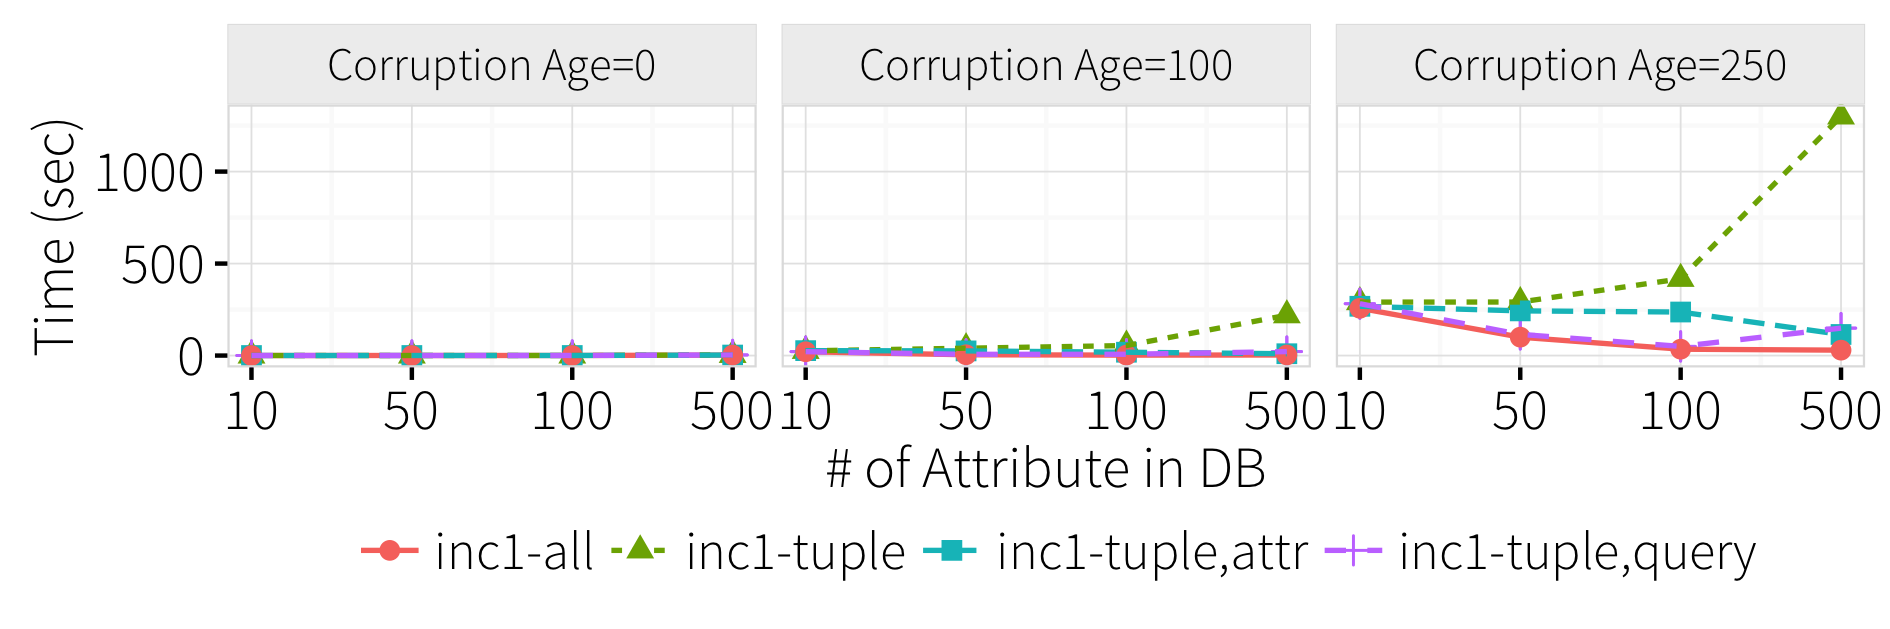
\includegraphics[width = .99\columnwidth]{figures/attr_time}
    \vspace*{-.1in}
    \caption{\# of attributes vs time.}
    \label{f:attr} 
    \end{subfigure}
    \begin{subfigure}[t]{.49\textwidth}
    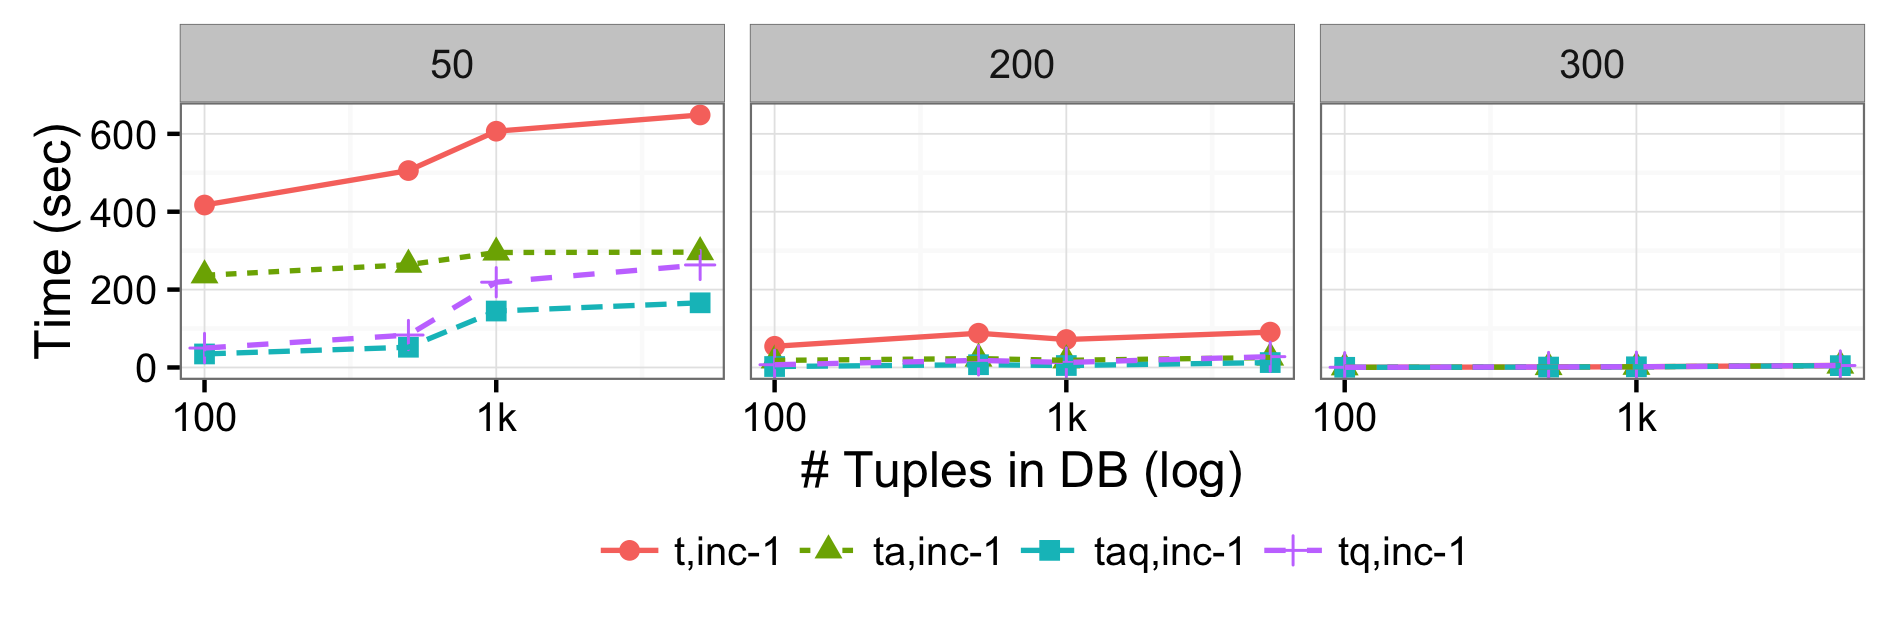
\includegraphics[width = .99\columnwidth]{figures/attr100_time}
    \vspace*{-.1in}
    \caption{Database size vs time ($N_a = 100$)}
    \label{f:attr100} 
    \end{subfigure}
    \vspace*{-.1in}
    \caption{For datasets with many attributes, the optimizations result in significant improvements.}
  \end{figure*}


In this section, we carefully study the performance and accuracy
characteristics of the basic MILP-based repair algorithm, 
slicing-based optimizations that improve the latency of the system, 
and the incremental algorithm for single query corruptions. 
Due to the difficulty of collecting corrupt query logs from active deployments, our goal instead is to understand these trade-offs in
controlled synthetic scenarios, as well as study the effectiveness
in typical database query workloads based on widely used benchmarks.

\looseness -1
\xlw{
To this end, our experiments are organized as follows: First, 
we compare the basic and incremental MILP algorithm against the different optimizations 
to highlight the value of different optimizations and the limitations of the basic approach. We then evaluate \sys using established database transaction benchmarks from OLTP-bench~\cite{difallah2013oltp}:
TPC-C~\cite{tpcc} and TATP~\cite{tatp}. In addition, we study the behavior of \sys using synthetic data sets and show that \texttt{UPDATE} queries are particularly difficult to repair and focus solely
on different types of \texttt{UPDATE}-only workloads to understand how \sys responds to different parameter settings.
We end with a discussion of \sys's capability in solving problems in more complex settings.}
All experiments were run on 12x2.66 GHz  machines with 16GB RAM running IBM CPLEX~\cite{cplex2014v12} as the MILP solver on CentOS release 6.6.







\subsection{Experimental Setup}


\iffalse
\begin{table}[t]\small
  \centering
  \begin{tabular}{@{}cll@{}}
  \toprule
  {\bf Param} & {\bf Description} & {\bf Default} \\ \midrule
  $V_d$  & Domain range of the attributes  & $[0, 100]$ \\
  $N_D$  & \# tuples in final database & $1000$ \\
  $N_a$  & \# attributes in database & $10$ \\
  $N_w$  & \# predicates in \texttt{WHERE} clauses & $1$ \\
  $N_s$  & \# \texttt{SET} clauses & $1$ \\
  $N_q$  & \# queries in query log & $300$ \\
  $idx$  & Index of corrupted query & $\{0, 25, 50,$ \\
         & (backwards from most recent) & $100, 200, 250 \}$ \\ 
  $r$    & Range size of \texttt{UPDATE} queries & 8 (tuples) \\
  $s$    & Zipf $\alpha$ param of query attributes, & $1$ \\ \bottomrule \end{tabular}
  \caption{Experimental Parameters}
  \label{t:params}
\end{table}
\fi


\iffalse
  \begin{table}[t]\small
    \centering
    \begin{tabular}{@{}cl@{}}
    \toprule
    {\bf Param} & {\bf Description} \\ \midrule
    $p$ & Precision: \% of repaired tuples that are correct. \\
    $r$ & Recall: \% of full complaint set repaired.\\
    $t_{total}$ & End-to-end execution time \\ 
    $d_{measure}$ & \red{Some sort of distance measure} \\ \bottomrule \end{tabular}
    \caption{Metrics Compared}
    \label{t:metrics}
  \end{table}
\fi



For each of our experiments we generate and corrupt a query log. 
We execute the original and corrupt query logs on an initial (possibly empty) database,
perform a tuple-wise comparison between the resulting database states to generate a true complaint set,
and simulate incomplete complaint sets by removing a subset of the true complaints.
Finally, we execute the algorithms and compare the repaired query log with the true query log, as well as the repaired and true
final database states, to measure performance and accuracy metrics.
Performance is measured as wall clock
time between submitting a complaint set and the system terminating after retrieving a valid repair.  
Accuracy is measured as the repair's precision (percentage of repaired tuples that were correctly fixed), 
the recall (the percentage of the full complaint set that was repaired), 
and the F1 measure (the harmonic mean of precision and recall).
We report the average across 20 runs.
We describe the experimental parameters in the context of the datasets and workloads below.





\stitle{Synthetic:} \label{sec:syntheticgen}
We generate an initial database of $N_D$ random tuples.  
The schema contains a primary key $id$ along with $N_a$ attributes $a_1\ldots a_{N_a}$, whose values are integers picked from $[0, V_d]$ uniformly at random.
We then generate a sequence of $N_q$ queries.
The default setting for these parameters are: $N_D = 1000, N_a = 10, V_d = 200, N_q = 300$.


\texttt{UPDATE} queries are defined by a SET clause that assigns an attribute a $Constant$ or $Relative$ value,
and a WHERE clause can either be a $Point$ predicate on a key, or a $Range$ predicate on non-key attributes:

{\scriptsize
\begin{verbatim}
 SET Clause:                WHERE Clause:
  Constant: SET (a_i=?), ..   Point: WHERE a_j=? & ..
  Relative: SET (a_i=a_i+?)   Range: WHERE a_j in [?,?+r] & ..\end{verbatim}}
\noindent where \verb|?|$\in [0, V_d]$ is random and \verb|r| is the size of the range predicate. 
Query selectivity is by default $2\%$ (\verb|r|$=4$).
Note that a range predicate where \texttt{r = 0} is distinct from a $Point$ predicate due to the non-key attribute.
The WHERE clauses in \texttt{DELETE} queries are generated in an identical fashion, while
\texttt{INSERT} queries insert values picked uniformly at random from $V_d$.
By default, we generate \texttt{UPDATE} queries with non-key range predicates and constant set clauses.
  
In addition, the skew parameter $s$ determines the distribution attributes referenced in the \texttt{WHERE} and \texttt{SET} clauses.  
Each attribute in a query is picked from either a uniform distribution when $s=0$ or a zipfian distribution with exponent $s$.
This allows our experiments to vary between a uniform distribution, where each attribute is
equally likely to be picked, and a skewed distribution where nearly all attributes are the same. 

\looseness -1
\stitle{Benchmarks: } We use the TPC-C~\cite{tpcc} and TATP~\cite{tatp} benchmarks.
The former generates the {\it ORDER} table at scale 1 with one warehouse, and uses the queries that modify the {\it ORDER} table. 
We execute a log of 1500 queries over an initial table containing 6000 tuples.  
$1837$ queries are \texttt{INSERT}s and the rest are \texttt{UPDATE}s. 
The latter TATP workload simulates the caller location system. 
We generate a database from {\it SUBSCRIBER} table with 5000 tuples and $1500$ \texttt{UPDATE} queries.
Both setups were generated using the OLTP-bench~\cite{difallah2013oltp}. 
We introduce a single corruption, and vary corrupted query's index from the most recent query $q_N$ to $q_{0}$.



\stitle{Corrupting Queries:} We corrupt query $q_i$ by replacing it with a randomly
generated query of the same type based on the procedures described above.
To standardize our procedures, we selected a fixed set of indexes $idx$
that are used in all experiments. 

\subsection{Benchmarks}
\label{sec:experiments:benchmark}
Figure~\ref{f:tpcctatp} plots the performance of the incremental algorithm using tuple-slicing on the TPC-C and TATP benchmark applications.  
The key reason is that each query affects a small set of records and leads to a very small complaint set---$1$ or $2$ on average.
In addition, tuple and query slicing can aggressively reduce the total number of constraints to a very small number---often less than $100$ in total.
Furthermore for TPC-C, the queries are predominantly \texttt{INSERT} queries, which \sys can solve within milliseconds. \xlw{TATP benchmark only contains \texttt{UPDATE} queries, which are harder to solve than \texttt{INSERT} queries and thus lead to higher execution time compared with TPC-C queries. }
Finally, we evaluated \sys on Example~\ref{ex:taxes} in Figure~\ref{fig:example} and fully repaired the correct query in 35 milliseconds. \sys's F1 score is nearly 1 across all benchmark experiments.
\ewu{Explain why TATP has a steeper slope than TPC-C} \xlw{done.}
\begin{figure}[h]
\centering
  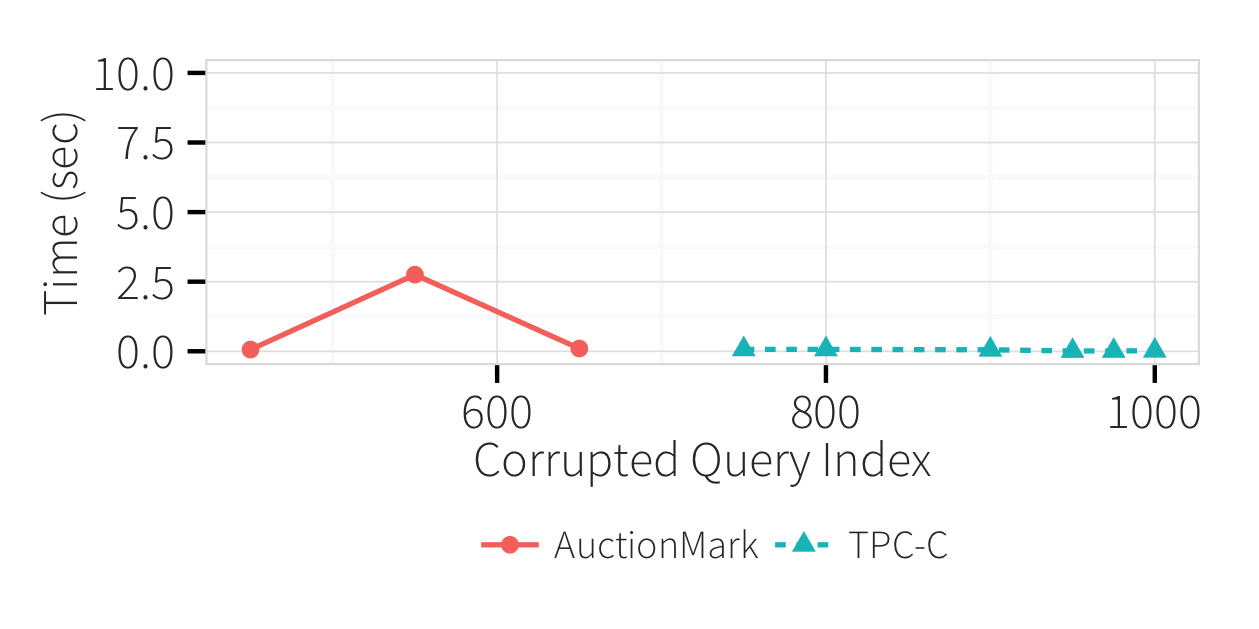
\includegraphics[width = .75\columnwidth]{figures/benchmark_time}
  \vspace*{-.2in}
  \caption{Our experiments on benchmark OLTP workloads show that \sys can produce repairs very fast.}
  \label{f:tpcctatp} 
\end{figure}

{\it Takeaways: many workloads in practice are dominated by \texttt{INSERT} and point \texttt{UPDATE} queries (ignoring the dominant percentage of read-only queries).  
In these settings, \sys is very effective at reducing the number of constraints and can derive repairs with near-interactive latencies.}





  \begin{figure*}[!htb]
    \hspace*{-.1in}
    \centering
     \begin{subfigure}[t]{.33\textwidth}
      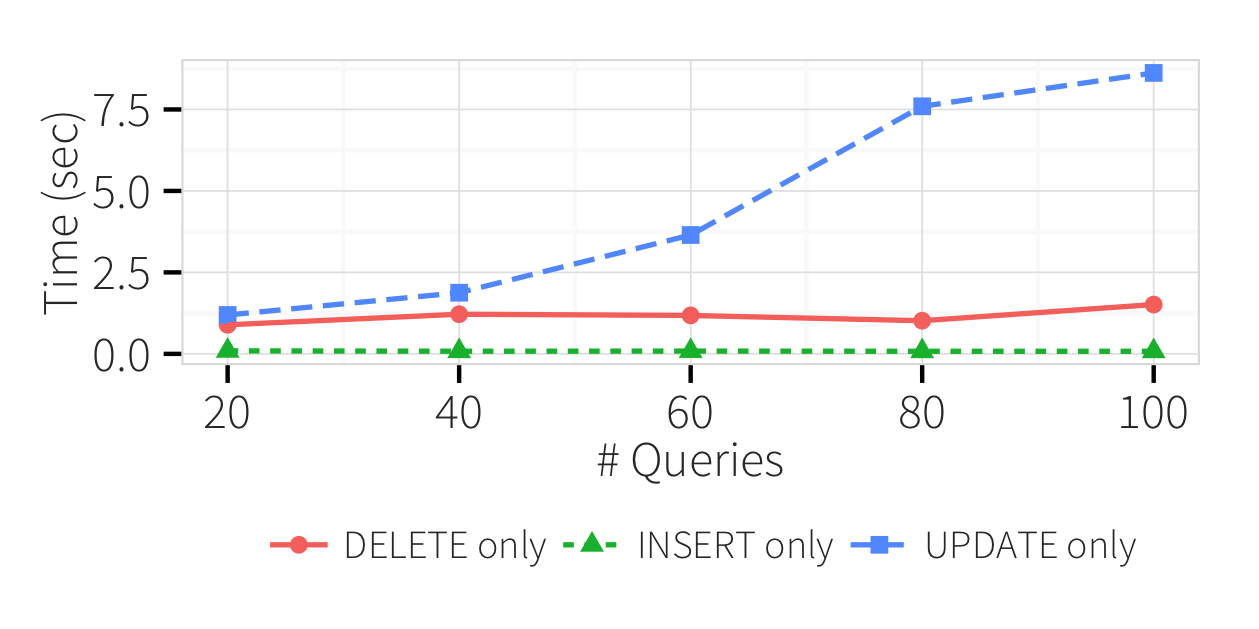
\includegraphics[width = .99\columnwidth]{figures/indelup_time}
      \caption{Performance for different query types.}
      \label{f:indelup_time} 
    \end{subfigure}
    \begin{subfigure}[t]{.33\textwidth}
      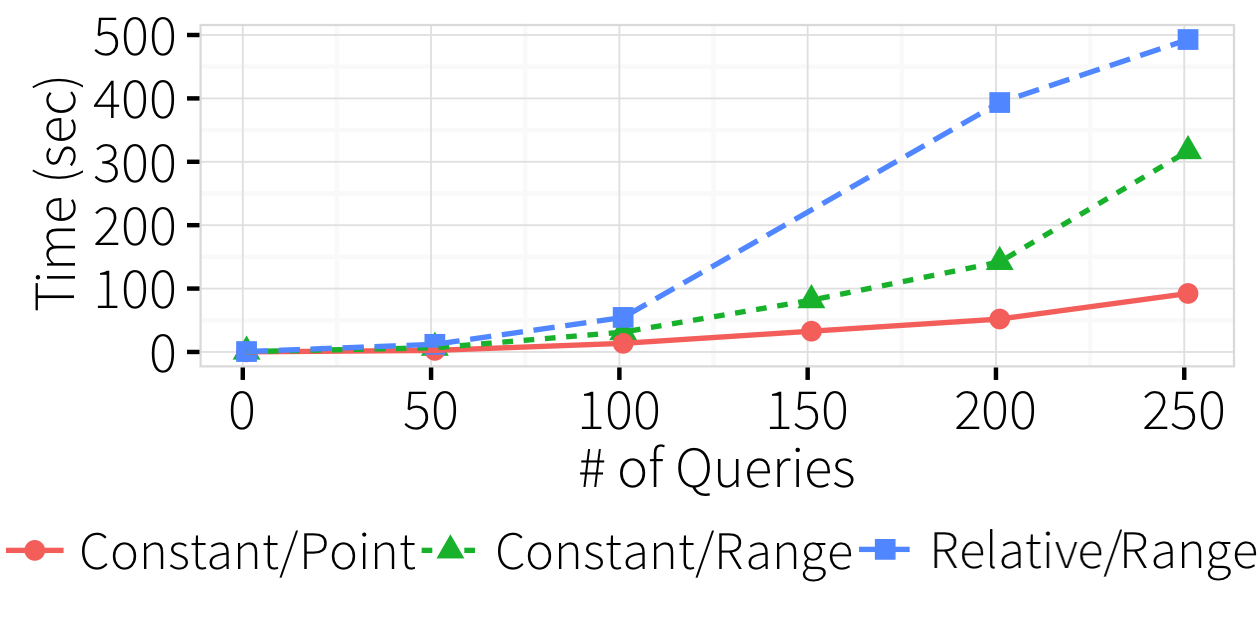
\includegraphics[width = .99\columnwidth]{figures/pointrelv_time}
      \caption{Performance of diff. query clause types.}
      \label{f:qidx_time} 
    \end{subfigure}
    \begin{subfigure}[t]{.33\textwidth}
      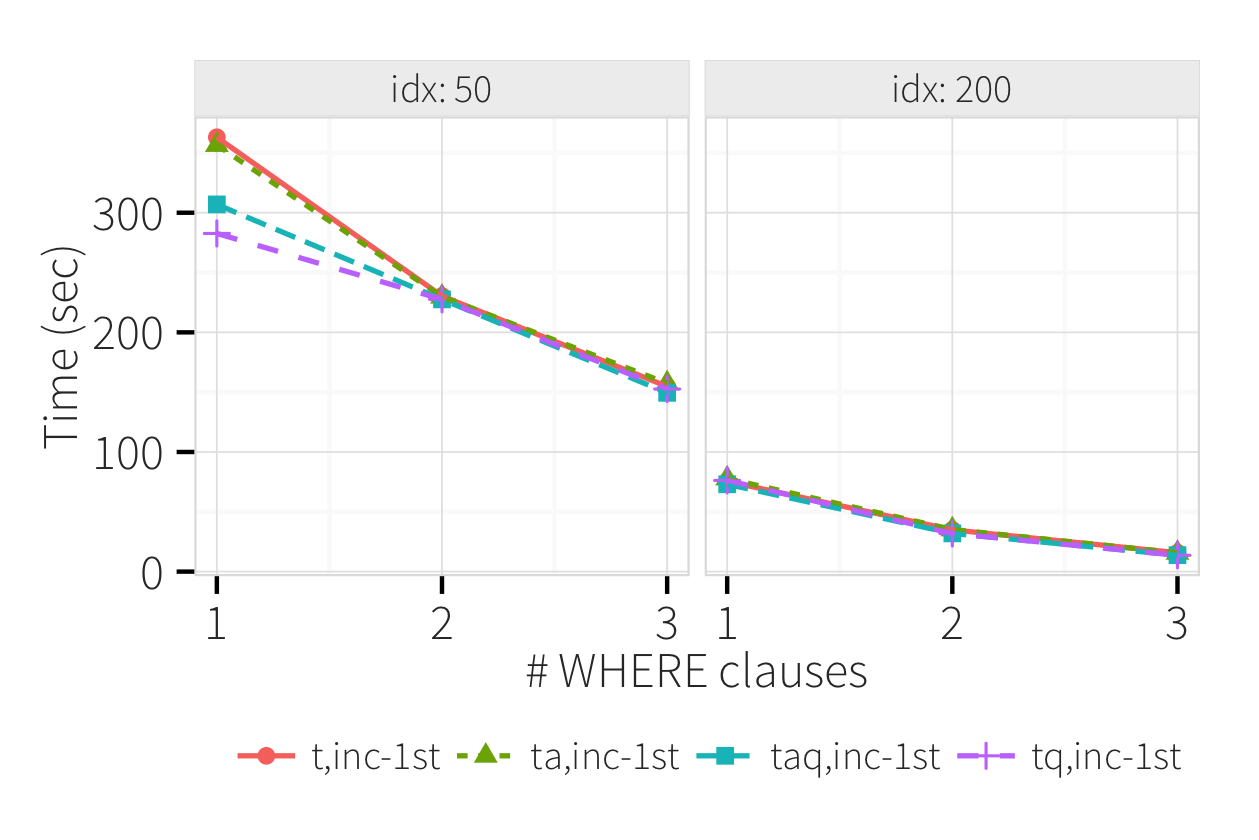
\includegraphics[width = .99\columnwidth]{figures/where_time}
      \caption{Query dimensionality vs time.}
      \label{f:where_time} 
    \end{subfigure}
    \caption{
    Performance and accuracy can be sensitive to some data and workload parameters, such as query skew, clause types, and dimensionality.  Notably, \sys can handle high false negative rates when the error resides in recent queries.}
  \end{figure*}



\subsection{Synthetic Incremental Experiments}
\subsubsection{Increasing the Hardness of Database}

\ewu{These are all increemental algorithms, not basic!  Need to explain what the names of each line means (e.g., inc1-all)} 
\xlw{done.}
  
\looseness -1
The following set of experiments are designed to establish the rationale for 
the settings in the subsequent experiments.  
\xlw{
Specifically, we compare different slicing-based optimizations of incremental repair (\emph{$Inc_1$})
as the hardness of database (number of attribute or database size) increases in the context of a single
corrupted query: \emph{inc1-all} as the incremental repair with all slicing optimization and \emph{inc-tuple/query/attr} as
the incremental repair with the corresponding tuple, query, and attribute slicing optimization. In addition, we omit the accuracy figures as the F1 score for all settings is nearly 1.}

\stitle{Increasing \# of Attribute :} \looseness -1
We first evaluate \sys and its optimizations by increasing the number of attribute ($N_a \in [10, 500]$) with $N_D = 100$.
As shown in Figure~\ref{f:attr}, when the number of attribute in a table is small (e.g., $N_a=10$) all algorithms appear identical. 
However, increasing the number of attribute exhibits a larger benefit for query and attribute slicing (up to $6.8\times$ reduction compared to tuple-slicing).
When the table is wide ($N_a = 500$), applying all optimizations ($inc_1-all$) is $40\times$ faster than \emph{tuple-slicing} alone.  


\stitle{Increasing Database Size:} \looseness -1
In Figure~\ref{f:attr100}, we vary the database size ($N_D \in [100,5000]$) with a large number of attributes ($N_a = 100$).
We fix the number of complaints by decreasing the query selectivity in proportion to $N_D$'s increase---the specific mechanism to do so does not affect the findings.
Figure~\ref{f:attr100} shows that the costs are relatively flat until the corruption occurs in an old query ($q_{50}$).  
In addition, we find that the cost is highly correlated with the number of candidate queries that are encoded in the MILP problem.
The increase in cost despite tuple-slicing is due to the increasing number of candidate queries in the system; 
we believe this increasing trend is due to the solver's ability to prune constraints that correspond to queries that clearly will not affect the complaint set---an implicit form of query slicing.  
Applying attribute-slicing supercedes this implicit optimization and results in a flat curve, 
while query-slicing explicitly reduces the number of candidate queries in proportion with the database size, and leads to the increasing trend.
Ultimately, combining all three optimizations improves the latency over tuple-slicing by $2\times$ in the worst case, and up to $4\times$ in the best case.

\smallskip
\textit{Takeaways: we find that the performance of the different repair algorithm 
heavily depends on the property of the datasets---in particular, the number of attributes and the number of tuples in the database. Tuple slicing is essential to solve general problems. Attribute and query slicing show significant gain for datasets with large number of attributes. }

\ewu{Need to introduce QFix again as setup for the subsequent experiments}
\xlw{Note that in both experiments, we omit the results of algorithms without applying tuple-slicing optimization as the these algorithms failed to scale over most of the problems. In the following experiments, we focus on studying the performance of a single \sys setting---incremental with tuple-slicing---on a narrow table setting that contains $N_a = 10$ attributes, and a single corrupt query in the query log.}


\subsubsection{Increasing the Hardness of Queries}
\label{sec:experiments:synth}
\xlw{
The following set of synthetic experiments evaluates \sys (incremental with tuple-slicing)'s performance while increase the hardness of queries by varying numerous workload parameters such as query type, query complexity, and log size $N_q$. Again, we skip the accuracy figures as \sys achieves near 1 F1 score in the following set of experiments. }

\iffalse
\emph{Database Size:} \looseness -1
Figure~\ref{f:dbsize_time} varies the database size ($N_D \in [100, 100k]$), and fixes query output cardinality and complaint set size in the same way as the previous scalability experiment.
In contrast to the previous experiment, the scalabality curve is nearly flat for both corruption query indices.
The reason is because the solver's implicit pruning optimization is less effective when there are only $10$ attributes: Every query is likely to touch an attribute that affects the complaint set.
We verified this by applyng query-slicing to the same setting, and found far fewer queries were pruned compared to the previous experiment.
It takes less than a minute to perfectly repair the recent corruption $q_{200}$,
and around $4$ minutes for the older corruption $q_{50}$, even as the database size increases.
At smaller database sizes, the randomness in the workload generator leads to variability in the size of the complaint set, and ultimately a larger and more difficult MILP problem.
The exponential relationship between solver time and problem difficulty results in the higher average latency for $q_{50}$.
\fi


\stitle{Query Type: }\label{sec:indelup}
This experiment evaluates the \sys 
($inc_1-tuple$) on \texttt{INSERT}, \texttt{DELETE}, or \texttt{UPDATE}-only workloads.
We increase the number of queries from $1$ to $200$ and corrupt the oldest query in the log.  
Figure~\ref{f:indelup_time} shows that while the cost of repairing \texttt{INSERT} workloads
remains relatively constant, the cost for \texttt{DELETE}-only and \texttt{UPDATE}-only workloads increase as 
the corruption happens earlier in the query log---and a much faster rate for \texttt{UPDATE} queries.

\ewu{Probably not needed at this point.  Maybe instead say "This is why we have focused on UPDATE queries in most of our experiments.}  We observe that \texttt{UPDATE} queries translate into more undetermined variables than other query types, and are significantly more expensive to repair. 
\iffalse
Based on these results, we focus on the incremental algorithm $inc_1$ and the more difficult \texttt{UPDATE}-only workloads in the rest of the experiments.
\fi

\smallskip
\stitle{Query Clause Type: }
So far, we have focused on \texttt{UPDATE} queries with constant set clauses and range predicates.  
Figure~\ref{f:qidx_time} individually varies each clause and compares against {\it Constant/Point} and {\it Relative/Range} queries. 
The x-axis varies the index of the corrupted query between $q_1$ and $q_{249}$.
We find that point predicates and constant set clauses are easier to solve than range predicates and relative set clauses, respectively.
The reason for the former pair is because range predicates double the number of undetermined variables as compared to point queries.  
In addition, point queries are on key attributes, thus further reduces the possible search space.  
We believe the latter pair is because the constant set clauses break the causal relationship between input and output records for the overwritten values.
This both simplifies the difficulty of the constraint problem, and reduces the total number of constraints.


\smallskip
\stitle{Predicate Dimensionality:}
Figure~\ref{f:where_time} varies the dimensionality of the update queries by increasing the number of predicates in the \texttt{WHERE} clause, while keeping the query cardinality constant.
The cost increases with the dimensionality because each additional predicate is translated into a new set of constraints and undetermined variables, increasing the problem complexity.
\ewu{Mention potential solutions to this issue}


\smallskip
\textit{Takeaways: we find that problems with \texttt{UPDATE}-workloads are significantly harder than problems with other types of queries. In addition, the performance of \sys also closely related to the complexity and the property of queries. 
\sys is able to solve hard problems (with ~$200$ \texttt{UPDATE}-only queries) in seconds or minutes---particularly if the error is recent. }


\subsection{Solving Hard Problems}
\label{sec:experiments:hardprob}

\ewu{Is this setion for "solving hard problems", or examining the limitations of basic on multi-query errors?} \xlw{This section is about examining \sys's limitations on two scenarios: incomplete complaint set information \& scalability over multi-query errors. Maybe we can change to section title as: Examining Limitations? or any other suggestions?}

In this section, we further study the performance of \sys in solving hard problems. In particular, we conduct two sets of experiments: the first experiment evaluate \sys with incomplete complaint sets; the second illustrate \sys's capability in handling multiple errors.
 
\stitle{Incomplete Complaint Set:} \looseness -1
The first experiment (Figures~\ref{f:falsenegative_time} and~\ref{f:falsenegative_acc}) varies the fase positive rate in incomplete complaint sets.
We increase the rate from $0$ ($0\%$ missing in the complaint set) to $.75$ ($75\%$ are missing).  
We find that reducing the size of the submitted complaint set naturally improves the repair performance,
however the repair quality, both precision and recall in Figure~\ref{f:falsenegative_acc}, may suffer if the corruption occured in a very old query. 
This is expected because \sys targets reported complaints, thus unreported complaints may easily be missed and lead to low recall.
In addition, despite the refinement step of tuple-slicing, the repair may over generalize and ``fix'' the wrong records, leading to low precision.


    
\begin{figure}[!htb]
  \hspace*{-.1in}
  \centering
    \begin{subfigure}[t]{.33\textwidth}
      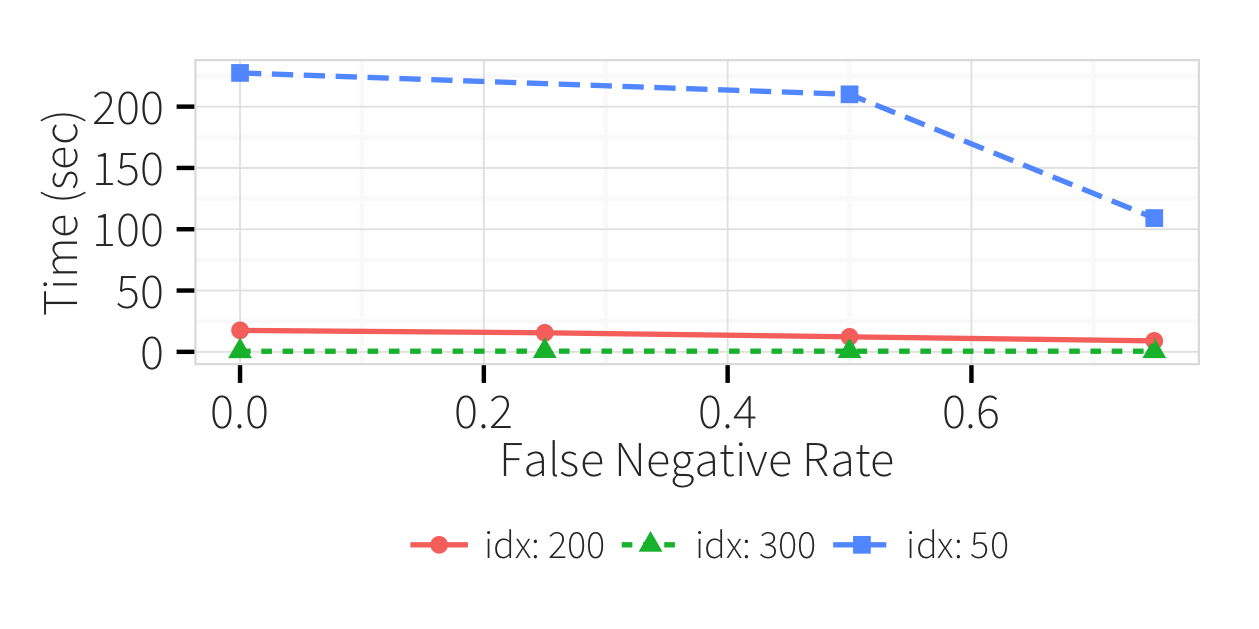
\includegraphics[width = .99\columnwidth]{figures/noise_fn_time} 
      \caption{False negatives vs time.}
      \label{f:falsenegative_time} 
    \end{subfigure}
    \\
    \begin{subfigure}[t]{.33\textwidth}
      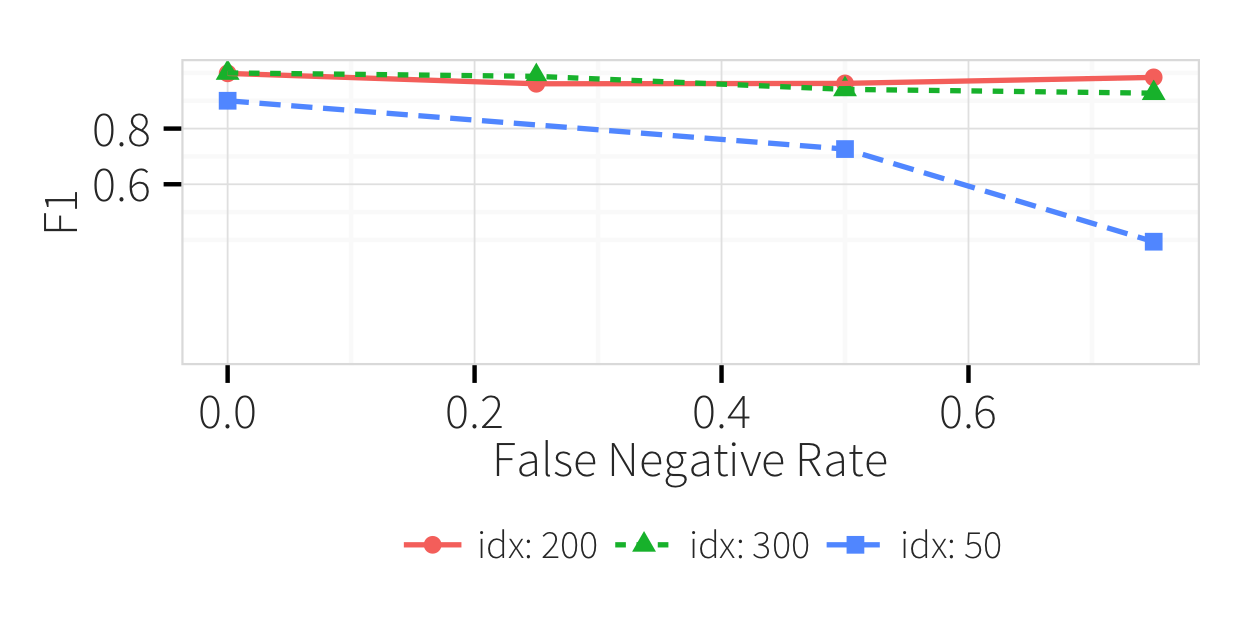
\includegraphics[width = .99\columnwidth]{figures/noise_fn_acc}
      \caption{False negatives vs accuracy.}
      \label{f:falsenegative_acc} 
    \end{subfigure}
    \vspace*{-.1in}
    \caption{Our analysis highlights limitations of \naive, the value of tuple-slicing, and the high cost of \texttt{UPDATE} queries.}
  \end{figure}

\iffalse
\emph{Skew:} We now study the effects of attribute skew on the algorithms.
We increase the skew parameter from $0$ (uniform) to $1$ (nearly every attribute is $A_0$) 
and find a reduction in latency (Figure~\ref{f:skew_time}).
We believe the reason is because increasing the skew focuses the query predicates over a smaller set of logical attributes, 
and increases the number of constraints placed on each of the logical attributes used in the query log.  
Each of these constraints reduces the search space of allowable values for that attribute, and thus simplifies the MILP problem.
This result suggests that \sys may be well suited for many transaction systems that naturally exhibit query skew.
Note that the overall number of constraints in the problem is the same, only their distribution over the query attributes has changed.
\fi


\stitle{Multiple Corrupt Queries:} \looseness -1
In the second experiment, we compare the basic approach (\naive) against 
each slicing optimization individually($basic-tuple, basic-attr, basic-query$).  
We use the default settings with $N_D = 1000$ tuples and a sequence of \texttt{UPDATE} queries.
We generate query logs in 5 different sizes $N_q\in \{10, 20, 30, 40, 50\}$ and corrupt 
every tenth query starting from oldest query $q_1$,
up to $q_{41}$.  For example, when the $N_q = {30}$, we corrupt 3 queries: $q_{1,11,21}$. 
We find that the number of queries greatly affects both the scalabality (Figure~\ref{f:multi_time}) 
and the accuracy (Figure~\ref{f:multi_acc}) of the algorithms. Specifically, as the number increases,
the number of possible assignments of the MILP parameters increases exponentially and the solver often takes
longer than our experimental time limit of $1000$ seconds and returns an infeasibility error.  
This is a predominant reason why the accuracy degrades past $30$ queries.  For example, 
when $40$ queries are involved (with $4$ corruptions) 
and we ignore the infeasible executions, the average execution time is $300$ seconds
and the precision and recall are greater than $0.94$.  Unfortunately, with $50$ queries ($5$ corruptions),
all runs exceed the time limit and return infeasibility.

  \begin{figure}[!htb]
  \hspace*{-.1in}
  \centering
    \vspace*{-.2in}
    \begin{subfigure}[t]{.33\textwidth}
    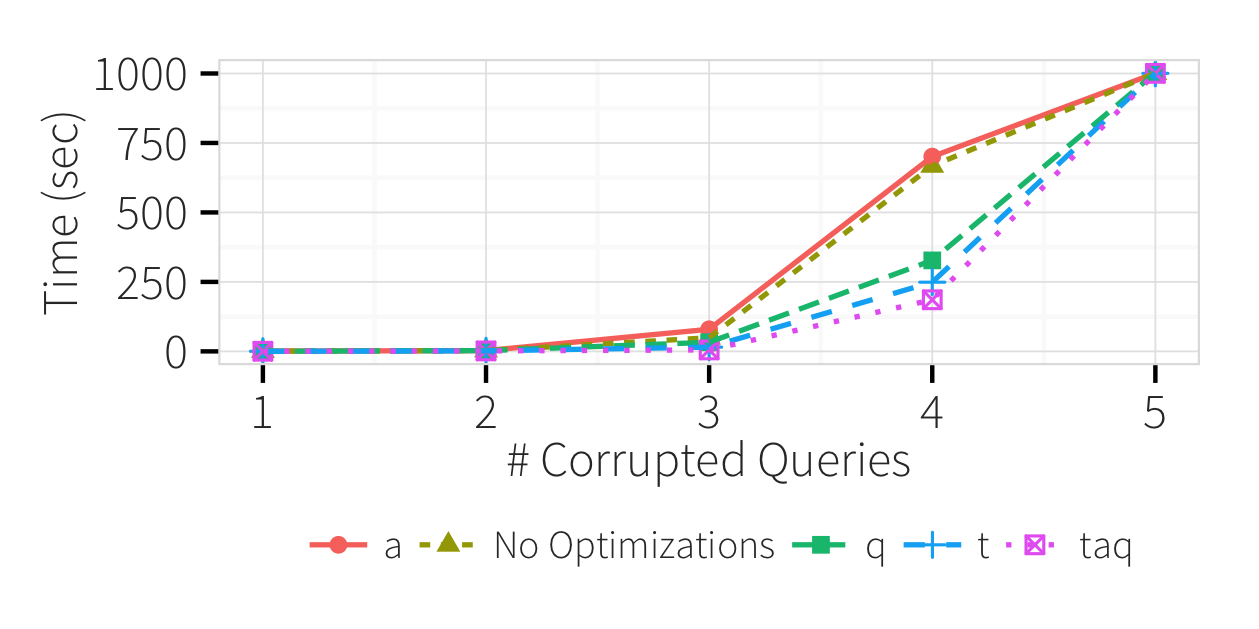
\includegraphics[width = .99\columnwidth]{figures/multi_time}
    \caption{Performance for multiple corruptions.}
    \label{f:multi_time} 
    \end{subfigure}
    \\
        \begin{subfigure}[t]{.33\textwidth}
    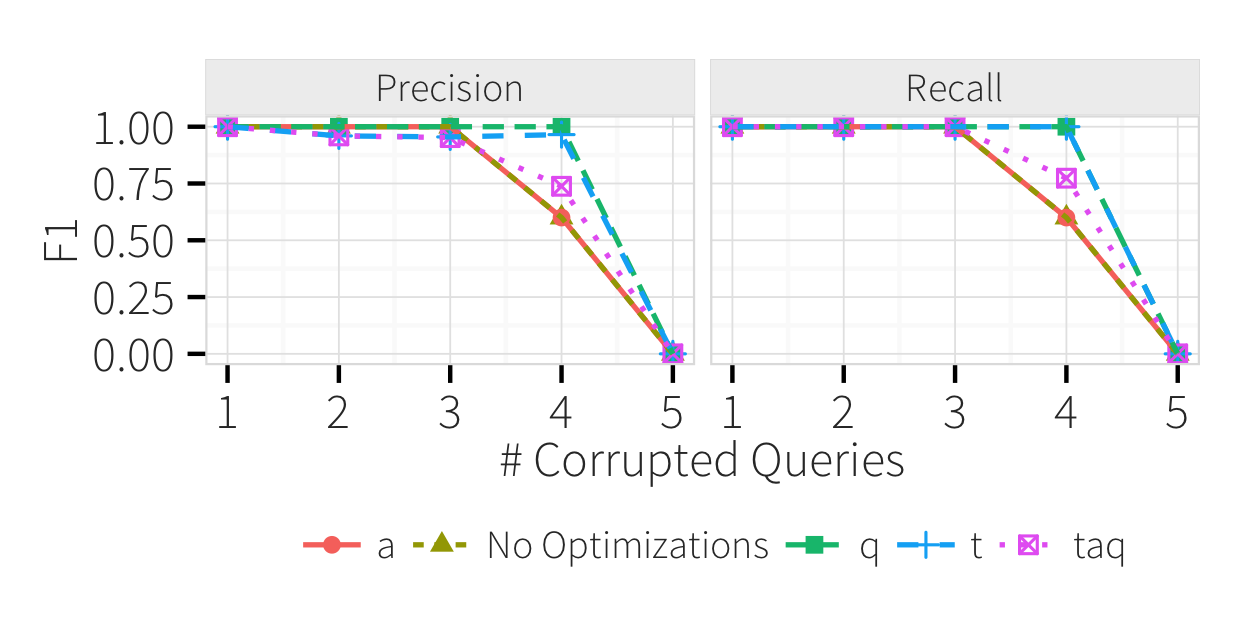
\includegraphics[width = .99\columnwidth]{figures/multi_pr}
    \caption{Accuracy for multiple corruptions.}
    \label{f:multi_acc} 
    \end{subfigure}
        \vspace*{-.1in}
    \caption{Our analysis highlights limitations of \naive, the value of tuple-slicing, and the high cost of \texttt{UPDATE} queries.}
  \end{figure}

\iffalse
\stitle{Single Corrupt Query:}
In this experiment, we evaluate the efficacy \sys with tuple slicing and incremental optimization
in the special case when one query has been corrupted in a much larger query log. 
We compare \incremental without tuple slicing ($inc_1$) against tuple slicing at 
different batching levels of 1, 2, 8 ($inc_1-tuple; inc_2-tuple, inc_8-tuple$). 
Recall from Section~\ref{sec:incremental} that $inc_k$ parameterizes $k$ consecutive queries in each batch until a repair is found.
Figure~\ref{f:singlequeryinc_time} highlights the scalability limitation of the incremental 
algorithm without tuple-slicing: with 50 queries $inc_1$  easily exceeds the 1000s limit.   
The tuple-slicing scales significantly better (nearly $200\times$ faster), however
the accuracy severely degrades when $k>1$.  
The primary reason is because of infeasibility errors---the MILP problem is much harder, and fails to find a repair.  
This is highlighted by the symmetry between the precision and recall curves.  
A secondary reason is beause the refinement step of  tuple slicing may not generate a fully correct repair and generalize incorrectly.
This is why the precision curve is lower than the recall curve for $inc_8-tuple$.
\fi


\smallskip
\emph{Takeaways: We observe \sys is able to solve recent errors (e.g., errors in most recent 100 queries) efficiently and effectively even with very limited information. Also, we find that basic, even with slicing optimizations, has severe scalability
limitations due to the large number of undetermined values-this is unsurprising as MILP constraint solving is an NP-hard
problem.
}



\section{Summary and discussion}

The general problem of data errors is highly complex, and exacerbated by its highly contextual nature.
We believe that an approach that explains and repairs such data errors based on operations performed by the application or user
is a promising step towards incorporating contextual hints into the analysis process.

Towards this goal, we presented \sys, the first framework to diagnose and
repair errors in the queries that operate on the data.
Datasets are typically dynamic: even if a dataset starts clean,
updates may introduce new errors. \sys can
analyze query logs to trace reported errors to the queries that
introduced them. This in turn helps identify additional errors
in the data that may have been missed and gone unreported.

We proposed a basic algorithm, \texttt{basic}, that uses non-trivial transformation rules to
encode information from the data and the query log as a MILP problem. We further improve 
\texttt{basic} with two types of optimizations: 
(1)~slicing-based optimizations that reduce the problem
size without compromising the accuracy, but rather often improving it, and 
(2)~an incremental approach that analyzes a single query at a time. 
Our experiments show that the latter
optimization can achieve significant scaling gains for single-query
errors, without significant reduction in accuracy.

To the best of our knowledge, \sys is the first formalization and solution to the diagnosis
and repair of errors using past executed queries. 
Obviously, correcting such errors in practice poses additional challenges. 
The initial version of \sys described in this paper focuses on a constrained problem consisting of
simple (no subqueries, UDFs, aggregations, nor joins)
single-query transactions with clauses composed of linear functions, and
complaint sets without false positives.
In future work, we hope to extend our techniques to relax these limitations.
In addition, we plan to investigate additional methods of scaling the constraint analysis, 
as well as techniques that can adapt the benefits of single-query analysis to errors in multiple queries.


\ewu{Say that this was largely simulated, and we want to move towards more realistic applications that have more complex query expressions, and how the queries interact with (simple) application logic is e.g., CRUD web applications}


%!TEX root = ../main.tex

\section{Related Work}
\label{s:related}

% data cleaning
\sys tackles the problem of diagnosis and repair in relational query
histories (query logs). It does not aim to correct errors in the data
directly, but rather to find the underlying reason for reported errors
in the queries that operated on the data. This is in contrast to
traditional data cleaning~\cite{rahm00, Raman01, Kalashnikov06,
Fan2008b} which focuses on identifying and correcting data
``in-place.'' Identifying and correcting errors is an important, and
rightfully well-studied problem. Existing literature has supplied a
variety of tools to capture errors originating from data
integration~\cite{Abiteboul99, Batini1986, Rahm2001, ParentS98},
recognizing the same entities in data~\cite{Koudas2006,
GruenheidDS14}, identifying true facts among conflicting
data~\cite{yin2008truth, DN09, ltm2012}, and language support for
cleaning~\cite{Galhardas2000}. All of these techniques are
complimentary to our work. Their goal is to identify which data is
correct and which data is incorrect, but they don't look for the
sources of these errors in the processes or queries that generate and
modify this data. In fact the output of such methods can be used to
augment the complaint sets used by \sys, which focuses on identifying
errors in the queries that produced the data, rather than the data
itself.

%repairs
An aspect of data cleaning focuses on providing repairs for the
identified errors~\cite{ChuIP13}. Tools in this domain have targeted
different methods and interactions for providing fixes, ranging from
functional dependencies~\cite{Fan2008b, ChuIP13} and
rules~\cite{Beskales2010, Cong2007} and functional
dependencies~\cite{Fan2008b, ChuIP13}, to interactive methods that
solicit user feedback~\cite{Yakout, Raman01}. As with the other data
cleaning approaches, all these techniques again operate on the data
directly. In contrast, \sys analyzes errors in the data to diagnose
and repair errors in queries that operated on the data. Thus, \sys
leverages the facts that some data errors are systemic, linked to
erroneous updates. Diagnosing the cause of the errors, will achieve
systematic fixes that will correct all relevant errors, even if they
have not been explicitly identified.

%% Data auditor and Data XRay
Closer to exploring systemic reasons and patterns for errors are
techniques such as Data Auditor~\cite{Golab2008, GolabKKS10} and Data
X-Ray~\cite{wang2015}. Both tools tools identify features, which can
be selected from the tuple attributes, that best summarize or describe
groups of tuples (or specifically errors). While these tools can
generate feature sets or patterns of attributes that characterize
errors, these are not linked to the queries, but are again
characterizations over the data itself. Such techniques can be
tremendously useful if the processes that generate or modify the data
are unknown or black-box computations. In these cases, Data Auditor
and Data X-Ray can provide high-level clues for potential problems in
the data derivation process. However, both approaches are oblivious to
the actual queries that operated on the data, and they do not provide
particular fixes. Ontology-based why-not
explanations~\cite{tenCate2015} is very similar to Data X-Ray, but is
only relevant to absent tuples (deletions), and again does not
consider the query history.



%things about diagnosis and explanations


\cite{Golab2008,GolabKKS10 } 

Studying and explaining
data outcome has been studied in many aspects:
\cite{GebalyAGKS14}
focuses on providing 
explanations to particular data outcome in tables; \cite{wang2015}
provides error diagnosing for general data extraction systems. 


% things  about validating updates before executing/cmmit to database
Related work about validating updates in time: 
\cite{Chen2011} validate correctness of updates before performing the update;


% things for exploring wrong or undetermined query,  why not? 
Related works on deriving desired select query: focus on 
Query by example, \cite{dimitriadou2014explore}  uses machine learning
techniques to explore query that satisfy user interests. 


% things about data provenance and data debugging
\cite{mucslu2013data}



Scorpion explanation uses data to synthesize predicates that explain.

Why not work.

View construction and query by example.

Take a look at temporal databases, the CIDR/arxiv paper has a few good starting points. Aditya also dug these out a while back


The way we return results is more like online aggregation or anytime algorithms -- 
as you run longer, the suggested fixes improve because we examine more of the query log.

\url{http://citeseerx.ist.psu.edu/viewdoc/download?doi=10.1.1.49.3765&rep=rep1&type=pdf}

\url{http://people.cs.aau.dk/~csj/Thesis/pdf/chapter26.pdf}

\balance

% Balancing columns in a ref list is a bit of a pain because you
% either use a hack like flushend or balance, or manually insert
% a column break.  http://www.tex.ac.uk/cgi-bin/texfaq2html?label=balance
% multicols doesn't work because we're already in two-column mode,
% and flushend isn't awesome, so I choose balance.  See this
% for more info: http://cs.brown.edu/system/software/latex/doc/balance.pdf
%
% Note that in a perfect world balance wants to be in the first
% column of the last page.
%
% If balance doesn't work for you, you can remove that and
% hard-code a column break into the bbl file right before you
% submit:
%
% http://stackoverflow.com/questions/2149854/how-to-manually-equalize-columns-
% in-an-ieee-paper-if-using-bibtex
%
% Or, just remove \balance and give up on balancing the last page.
%


\newpage
{
% If you want to use smaller typesetting for the reference list,
% uncomment the following line:
% \small
%\bibliographystyle{acm-sigchi}
\bibliographystyle{abbrv}
\bibliography{main}
}

\techreport{
\appendix

\section{A Learning-based Approach}
\label{sec:heuristic}
  
A drawback of the MILP approach is that the generated models grow with the 
size of the database and query log.
However, we argue that the encoded information is necessary in order to generate a sufficient set of constraints that result in a good repair.
In this section, we examine an alternative, simpler, decision tree-based approach called \dt. 
We show that even in a simple case of a single query log and a complete complaint set, it is expected to perform poorly.
We will first describe how to model the repair process using a decision tree,
and then we will present and discuss experimental results that illustrate its limitations.

\subsection{Modeling Repairs with Decision Trees}

Rule-based learners are used in classification tasks to generate a set of rules, or conjunctive predicates that best classify a group of labeled tuples.
The rules are non-overlapping, and each is associated with a label---a tuple that matches a given rule is assigned the corresponding label.
These rules exhibit a natural parallel with SQL \texttt{WHERE} clauses, 
which can be viewed as labeling selected tuples with a positive label and rejected tuples with a negative label.
Similarly, the structure of the rules is identical to those that \sys is designed to repair.
Thus, given the database tuples labeled to describe the errors, we may use a rule-based learner to
generate the most appropriate \texttt{WHERE} clause.
We focus our attention on rule-based learners;
specifically, we experiment with the C4.5~\cite{quinlan1987} decision tree learner, which is an 
exemplar of rule-based learners.

A core limitation of this classification-based approach is that there is no means to 
repair \texttt{SET} clauses, which modify data values rather than simply label them.
We resolve this with a two step approach.
We first use the decision tree to generate a repair for the
\texttt{WHERE} clause, and then use the modified query to identify repairs for the \texttt{SET} clause.
The need for this two step procedure limits this approach to encoding and repairing at most one query
at a time.

\noindent
\textbf{Repairing the WHERE Clause:}
The \texttt{WHERE} clause of an update query is equivalent to a
rule-based binary classifier that splits tuples into two groups:
(1)~tuples that satisfy the conditions in the \texttt{WHERE} clause
and (2)~tuples that do not. A mistake in a query predicate can 
cause a subset of the tuples to be misclassified, and in turn,
translate into data errors. 
Therefore, repairing the complaints corresponds to repairing the imprecise classification. 

The repair works as follows: For an incorrect query $q$, let
$D_0$ be the database state before $q$, and $D_1^*$ the \emph{correct}
database state that should have been the result after $q$, if $q$ were correct.
We use each tuple $t \in D_0$ as an element in the input training data
for the classifier where the values (of each attribute) of $t$ define
the feature vector and the label for $t$:
	\[
    label(t)= 
    \begin{cases}
    true & \textrm{if\ }D_0.t \neq D_1^*.t\\
    false              & \text{otherwise}
    \end{cases}
\]
The \texttt{true} rules generated by the decision tree trained on this labeled dataset 
forms a disjunction of rules that constitute the repaired \texttt{WHERE} clause.


\noindent
\textbf{Repairing the SET Clause:}
The \texttt{WHERE} clause repair proposed by the classifier may not completely repair 
the complaints if there was also an error in the \texttt{SET} clause. 
In this case, we execute a second repair step.
\begin{figure}[htb]
\centering
  \begin{subfigure} [t]{.75\columnwidth}
  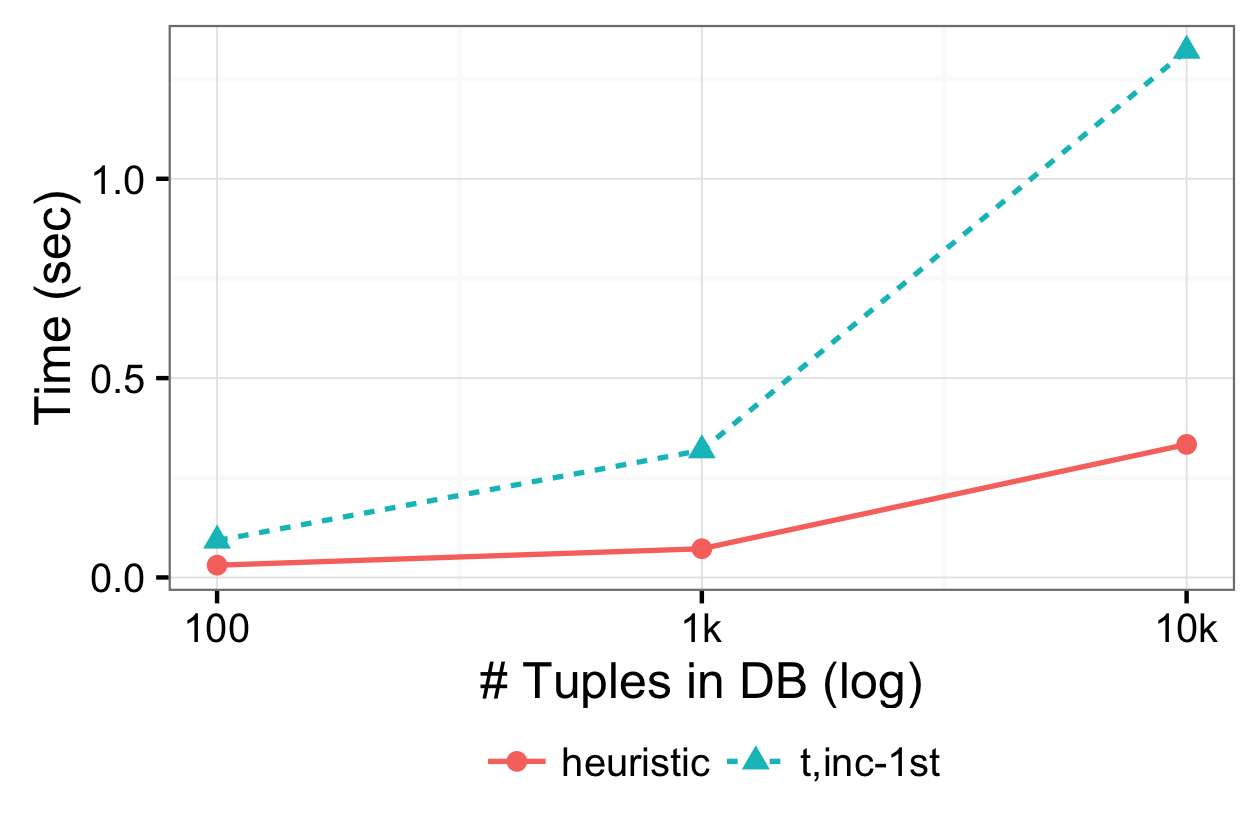
\includegraphics[width = \columnwidth]{figures/heuristictime}
  \caption{Comparison on Performance.}
  \label{f:heuristic_time} 
  \end{subfigure}\\

  \begin{subfigure} [t]{.75\columnwidth}
  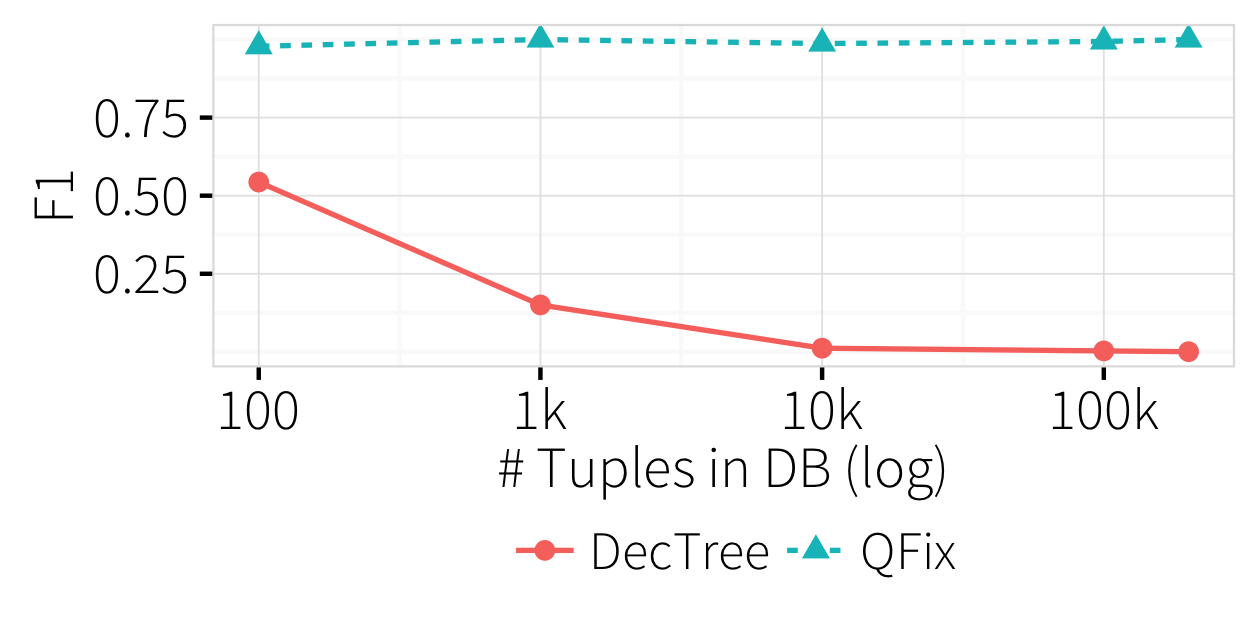
\includegraphics[width = \columnwidth]{figures/heuristicacc}
  \caption{Comparison on Accuracy.}
  \label{f:heuristic_acc} 
  \end{subfigure}
 \caption{\dt compared with \sys}
 \label{f:heuristic}
\end{figure}

We model the errors as a simple linear system of equations: 
each expression in the \texttt{SET} clause is translated into a
linear equation in the same fashion as described in Section~\ref{sec:sol}.
Directly solving the system of equations for the undetermined variables 
will generate the desired repair for the \texttt{SET} expression.



\subsection{Experimental Results}

To illustrate these shortcomings, we compare \dt with \sys using a simplified version of the setup from Section~\ref{sec:experiments} that favors \dt.
We restrict the query log to contain a single query that is corrupted, use a complete complaint set  and vary the database size.
We use the following query template, where all \texttt{SET} clauses assign the attributes to constants,
and the \texttt{WHERE} clauses consist of range predicates:

{\scriptsize
\begin{verbatim}
  UPDATE table
  SET  (a_i=?), ...
  WHERE a_j in [?,?+r] AND ...
\end{verbatim}
}

Figure~\ref{f:heuristic_time} shows that although the runtime performance of \dt is better than \sys by small a constant factor ($\sim 2.5 \times$),
both runtimes degrade exponentially.
In addition, the \dt repairs are effectively unusable as their accuracy is low: the F1-score starts at $0.5$ and rapidly degrades towards $0$.
From these empirical results, we find that \dt generates low-quality repairs even under the simplest conditions---an approach
that applies \dt over more queries is expected to have little hope of succeeding.



There are three important reasons why \dt, and any approach that focuses on a single query at a 
time\footnote{Although our incremental approach tries to generate a repair for a single
query at a time, it encodes all subsequent queries in the log.}, will not perform well.

\iffalse
  \begin{figure*}[t]
  \centering
      \begin{subfigure} [t]{.3\textwidth}
    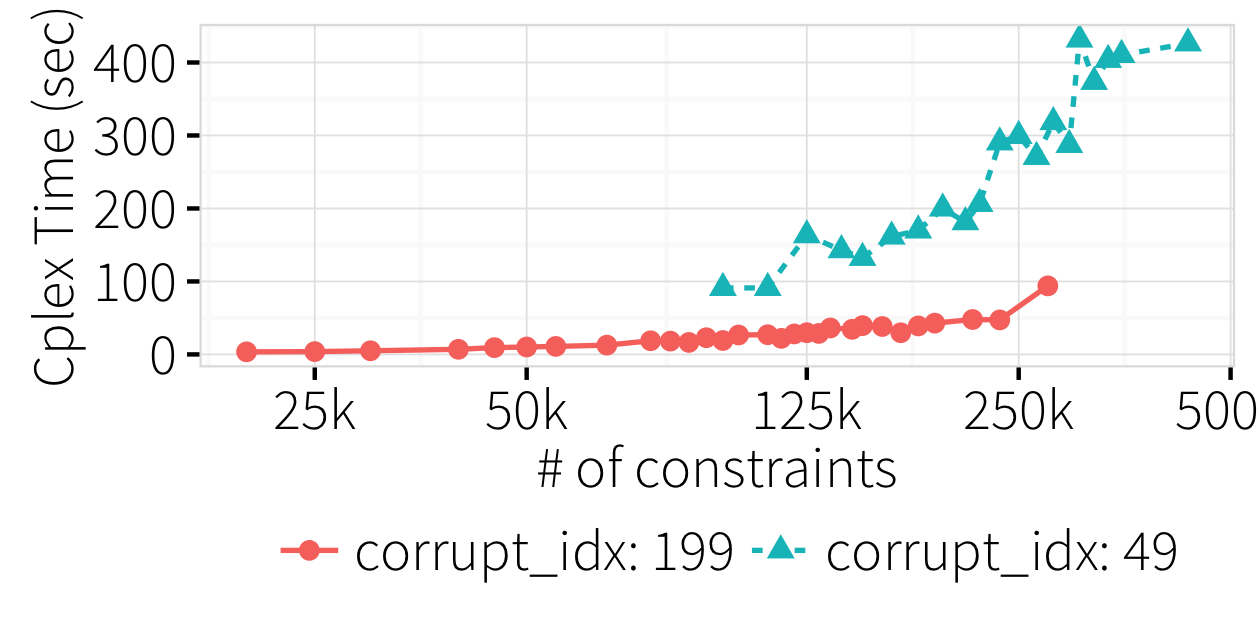
\includegraphics[width = .99\columnwidth]{figures/num_cons_time}
    \vspace*{-.25in}
    \caption{\# of constraints vs. solver solving time.}
    \vspace*{-.1in}
    \label{f:cons_vs_time} 
    \end{subfigure}
    \begin{subfigure} [t]{.3\textwidth}
    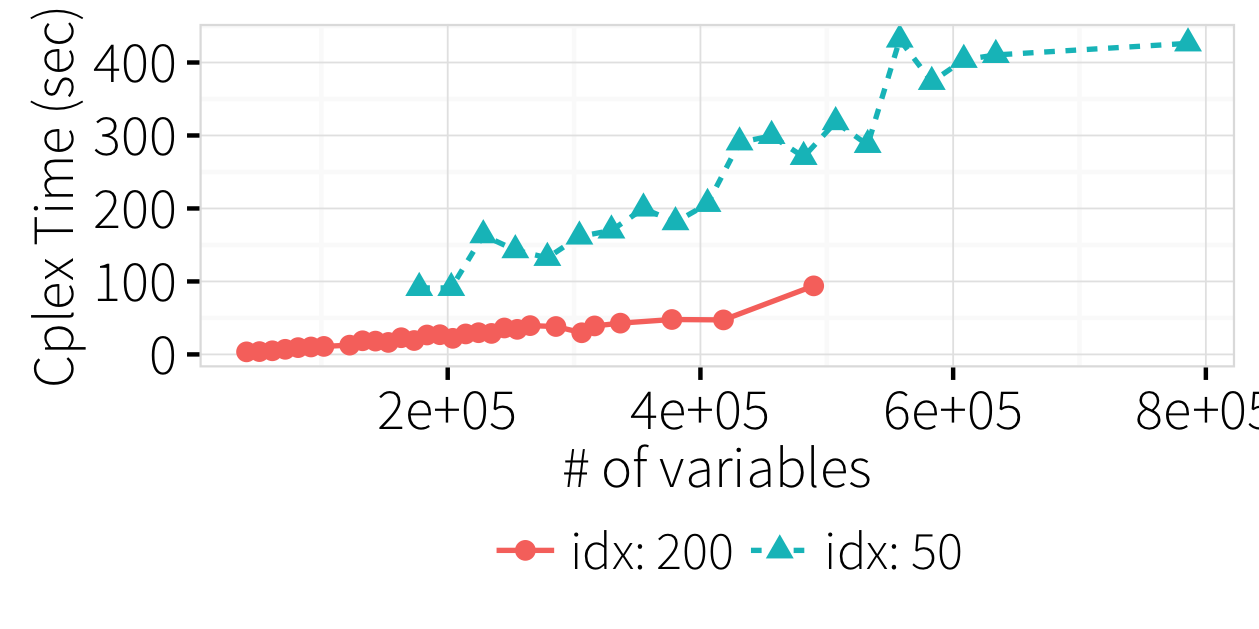
\includegraphics[width = .99\columnwidth]{figures/num_vars_time}
    \vspace*{-.25in}
    \caption{\# of undetermined variables vs. solver solving time.}
    \vspace*{-.1in}
    \label{f:var_vs_time} 
    \end{subfigure}
    \begin{subfigure} [t]{.3\textwidth}
    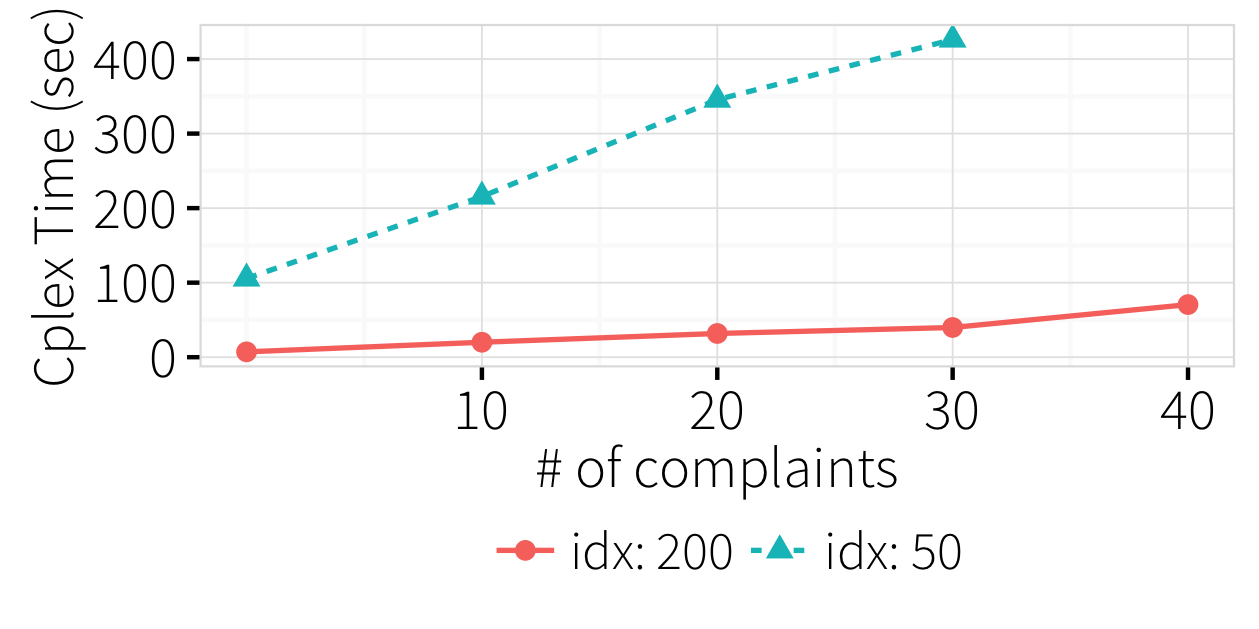
\includegraphics[width = .99\columnwidth]{figures/num_compl_time}
    \vspace*{-.25in}
    \caption{\# of compl. vs. solver solving time.}
    \vspace*{-.1in}
    \label{f:compl_vs_time} 
    \end{subfigure} 
    \iffalse
    \begin{subfigure} [t]{.3\textwidth}
    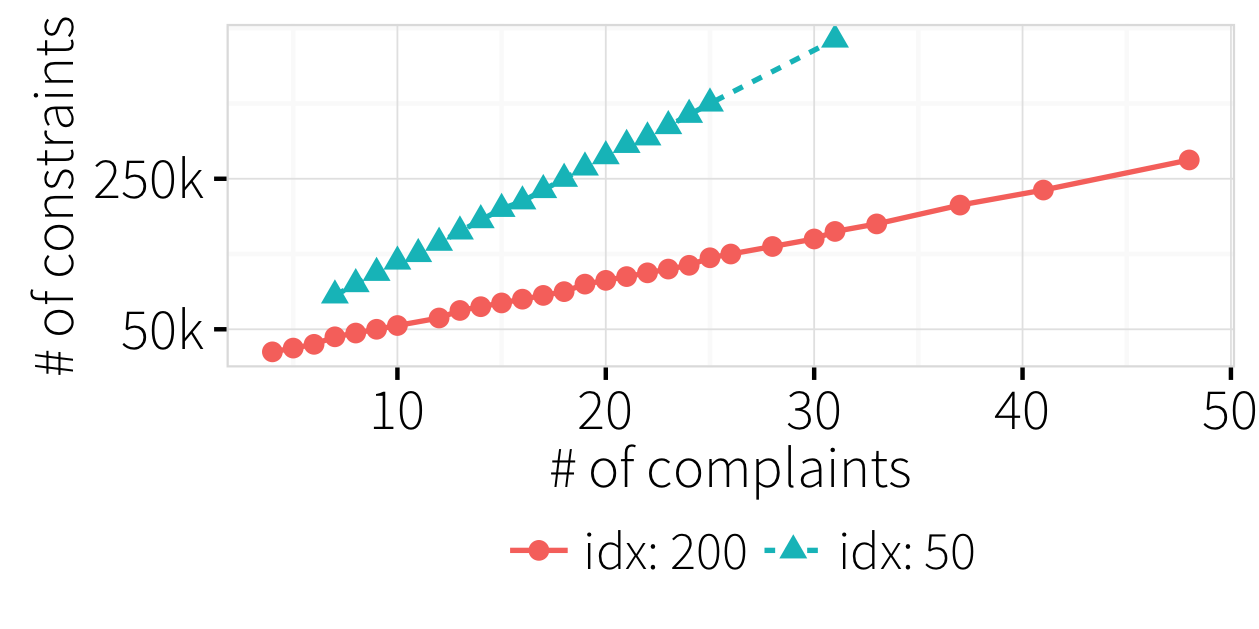
\includegraphics[width = .99\columnwidth]{figures/num_compl_cons}
    \vspace*{-.25in}
    \caption{\# of constraints vs.\# of compl.}
    \vspace*{-.1in}
    \label{f:compl_vs_cons} 
    \end{subfigure}
    \begin{subfigure} [t]{.3\textwidth}
    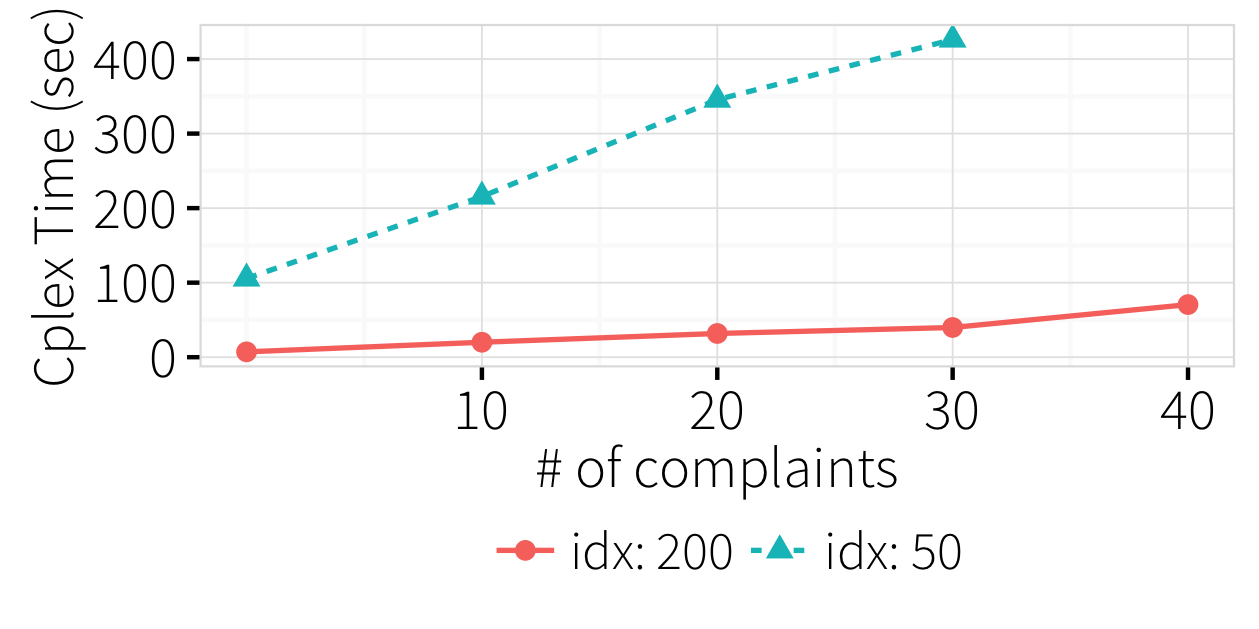
\includegraphics[width = .99\columnwidth]{figures/num_compl_time}
    \vspace*{-.25in}
    \caption{\# of undetermined variables vs. \# of compl.}
    \vspace*{-.1in}
    \label{f:compl_vs_time}
    \end{subfigure}
    \fi
   \caption{Solver solving time grows with all three factors: number of constraints, number of undermined variables and number of complaints. }
   \vspace*{-.1in}
   \label{f:soltime}
  \end{figure*}
\fi
\begin{itemize}[itemsep=1pt, leftmargin=5mm]
\item \textbf{Single Query Limitation: }
In principle, one could attempt to apply this technique to the
entire log one query at a time, starting from the most recent query.
Even ignoring the low repair accuracy shown in Figure~\ref{f:heuristic_acc},
this approach is infeasible.
Consider that we generate a labeled training dataset to repair $q_i$ 
using the query's input and output database states $D_{i-1}$ and $D_i^*$.
Note that $D_i^*$ is the theoretically \emph{correct} database state assuming no errors in the query log.
We would need to derive $D_i^*$ by applying the complaint set to $D_n$ to create $D_n^*$, and roll back the database state.
Unfortunately, \texttt{UPDATE} queries are commonly surjective such
that their inverses are ambiguous, which means that it is often
impossible to derive $D_i^*$. In contrast, the incremental version of
\sys can bypass this problem by encoding subsequent queries in the log
in a MILP representation.


\item \textbf{Structurally Different \texttt{WHERE} Clause Results: } 
The basic classifier approach simply learns a set of rules to minimize
classification error, and can derive a clause whose struture is arbitrarily 
different from the original query's \texttt{WHERE} clause.
Although it may be possible to incorporate a distance measure as part of the decision tree
splitting criteria, it is likely to be a heuristic with no guarantees.


\item \textbf{High Selectivity, Low Precision: }
Classifiers try to avoid overfitting by balancing the complexity of the rules with classification accuracy.
This is problematic for highly selective queries (e.g., primary key updates), because the classifier
may simply ignore the single incorrect record and generate a rule such as \texttt{FALSE}.
In fact, this form of severely imbalanced data continues to be a challenge for most major classification algorithms~\cite{he2009learning, galar2012review}. 
Thus, we believe that alternative classification algorithms would not improve on these results. 
Compound with the fact that many workloads are primarily composed of
key update queries~\cite{oltpbench} this issue severely limits the
applicability of learning-based approaches.

\end{itemize}





\iffalse


\section{MILP Solver Performance}
\label{app:solvtime}

Some background about why we are runnig these experiments.  What is known about MILP solvers already.

\subsection{Factors Relevant to Solver Performance}

\ewu{reference other constraint performance papers}
In this section, we study factors that influence the MILP solver solving time. In this paper, we
use IBM CPLEX~\cite{cplex2014v12} as a black box to solve the constructed MILP problems.  \ewu{describe MILP problems to justify why we focus on num constraints and num variables.} Similar to many solver performance studies~\cite{atamturk2005integer, meindl2012analysis, gearhart2013comparison}, 
we majorly study the connection between solver performance between \textit{the number of constraints} and \textit{the number of variables} in the constructed MILP problem. For this, we create \texttt{UPDATE}-only workloads using our synthetic data generator for 300 queries with constant \texttt{SET} clause and range \texttt{WHERE} clause: 

{\scriptsize
\begin{verbatim}
  UPDATE table
  SET  (a_i=?), ...
  WHERE a_j in [?,?+r] AND ...
\end{verbatim}
}
We further corrupt two query indexes, $q_{50}$ and $q_{200}$, to create the dirty query logs. \xlw{We only show results for  \texttt{UPDATE}-only workloads since all types of workloads show similar correlations. In addition, the selected corrupt query indexes allow us to evaluate the solver performance over median to large problem sizes.}  \ewu{We chose these because...} 


\smallskip
\emph{Number of Constraints: } We first study the relationship between solver performance and number of constraints. \xlw{The number of constraints is controlled via multiple factors including the number of complaints, corrupt query index, complexity of queries. Due to the randomness in synthetic data generator, we are not able to control the size of constraints to a specific value.} \ewu{Explain that the number of constraints is not controlled by you, which is why the lines start and end at different values in the figures.} From Figure~\ref{f:cons_vs_time}, we observe that solver time is roughly positive proportional, with tiny fluctuation, to the number of constraints in both corrupt indexes. This is expected because increasing the number of constraints by large scale usually accompany with significantly greater amount of variables in the MILP problem, which lead to harder MILP problems by natural. However, MILP problems \ewu{cite MILP papers that say this, so it's clear we are describing well known problems} with slightly larger amount of constraints sometimes could be even easier to solve since the additional constraints help pruning the searching space for similar amount of variables.

\smallskip
\emph{Number of Variables: } Similar to the previous experiment, we next compare the solver time with the number of variables. As shown in Figure~\ref{f:var_vs_time}, we find highly correlated trends compare to Figure~\ref{f:cons_vs_time}. 
This is due to the way we construct the MILP problem: the number of constraints and the number of variables grows linearly with \textit{the number of queries and the number complaints}.  



\iffalse
 In our experiments we found that increasing the number of constraints by increasing the database, query log, or complaint set sizes aversely affects the solver performance,
  solver performance has been shown to \emph{improve} as constraints that effectively reduce the problem space are added to the problem.  
  Thus, we now focus on the effects on the number of undetermined variables, which strictly increases the problem space.
  We keep the number of constraints fixed, however increase the number of undetermined variables by \ewu{XL fill in}. \xlw{need to rerun exp to get required numbers. We need to gradually increase the batch size to achieve this. }

\fi

In Figure~\ref{f:compl_vs_time} we illustrate the above argument by comparing the average solver time between the number of complaints at two different corrupt indexes. This allows us to study the relationship between solver time with both the number of complaints (x-axis) and the number of queries (two indexes). As expected, with the same number of complaints, the solver solving time for corrupt index $50$ is significantly higher than index $200$ since the number of queries encoded in each problem is $250$ and $100$ respectively. In contrast, with the same corrupt query index, problems with higher amount of complaints has much higher average solver solving cost than problems with lower amount of complaints. We believe that this is because increasing the number of queries and the number of complaints would increase both the number of variables and constraints in the constructed MILP problem. 

\xlw{The number of variables and constraints are two quantifiable factors that influence the solver time in solving MILP problems. However, there are other non-quantifiable factors, including but not limited to the correlations among variables, searching space of under-determined variables after pre-processing, that also relevant to the hardness of the MILP problem, which determines the solver time. These non-quantifiable factors are hard to control and optimize. Thus, in this paper, we mainly focus on optimizing (reducing) the quantifiable factors -- number of variables and constraints in order to reduce the  solver time. }

\subsection{Factors Relevant to the Number of Complaints}

From the above experiments, we observe that the solver time is highly correlated to the number of complaints and the number of queries we encoded in a MILP problem. The number of queries can be easily controlled by a particular parameter $N_q$. The number of complaints, on the other hand, is a reflection of the queries that have run over the database. It is influenced by  factors including the \texttt{SET} clause type, corrupt query index, query skewness, \texttt{WHERE} clause range, and some random factors. \ewu{however, don't know how the affect the complaint set.}  To better understand factors that control the size of the complaint set, we ran simulations using a database with $20$ attributes, and a query log of size $1000$ containing
either all constant or relative \texttt{SET} clause \texttt{UPDATE} queries. We found that SET and relative queries behave differently.
We varied the number of corrupt index uniformly throughout the query log, and additionally varied
the skew and range parameters to study how they affect the size of the complaint sets.



\begin{figure}[h]
\centering
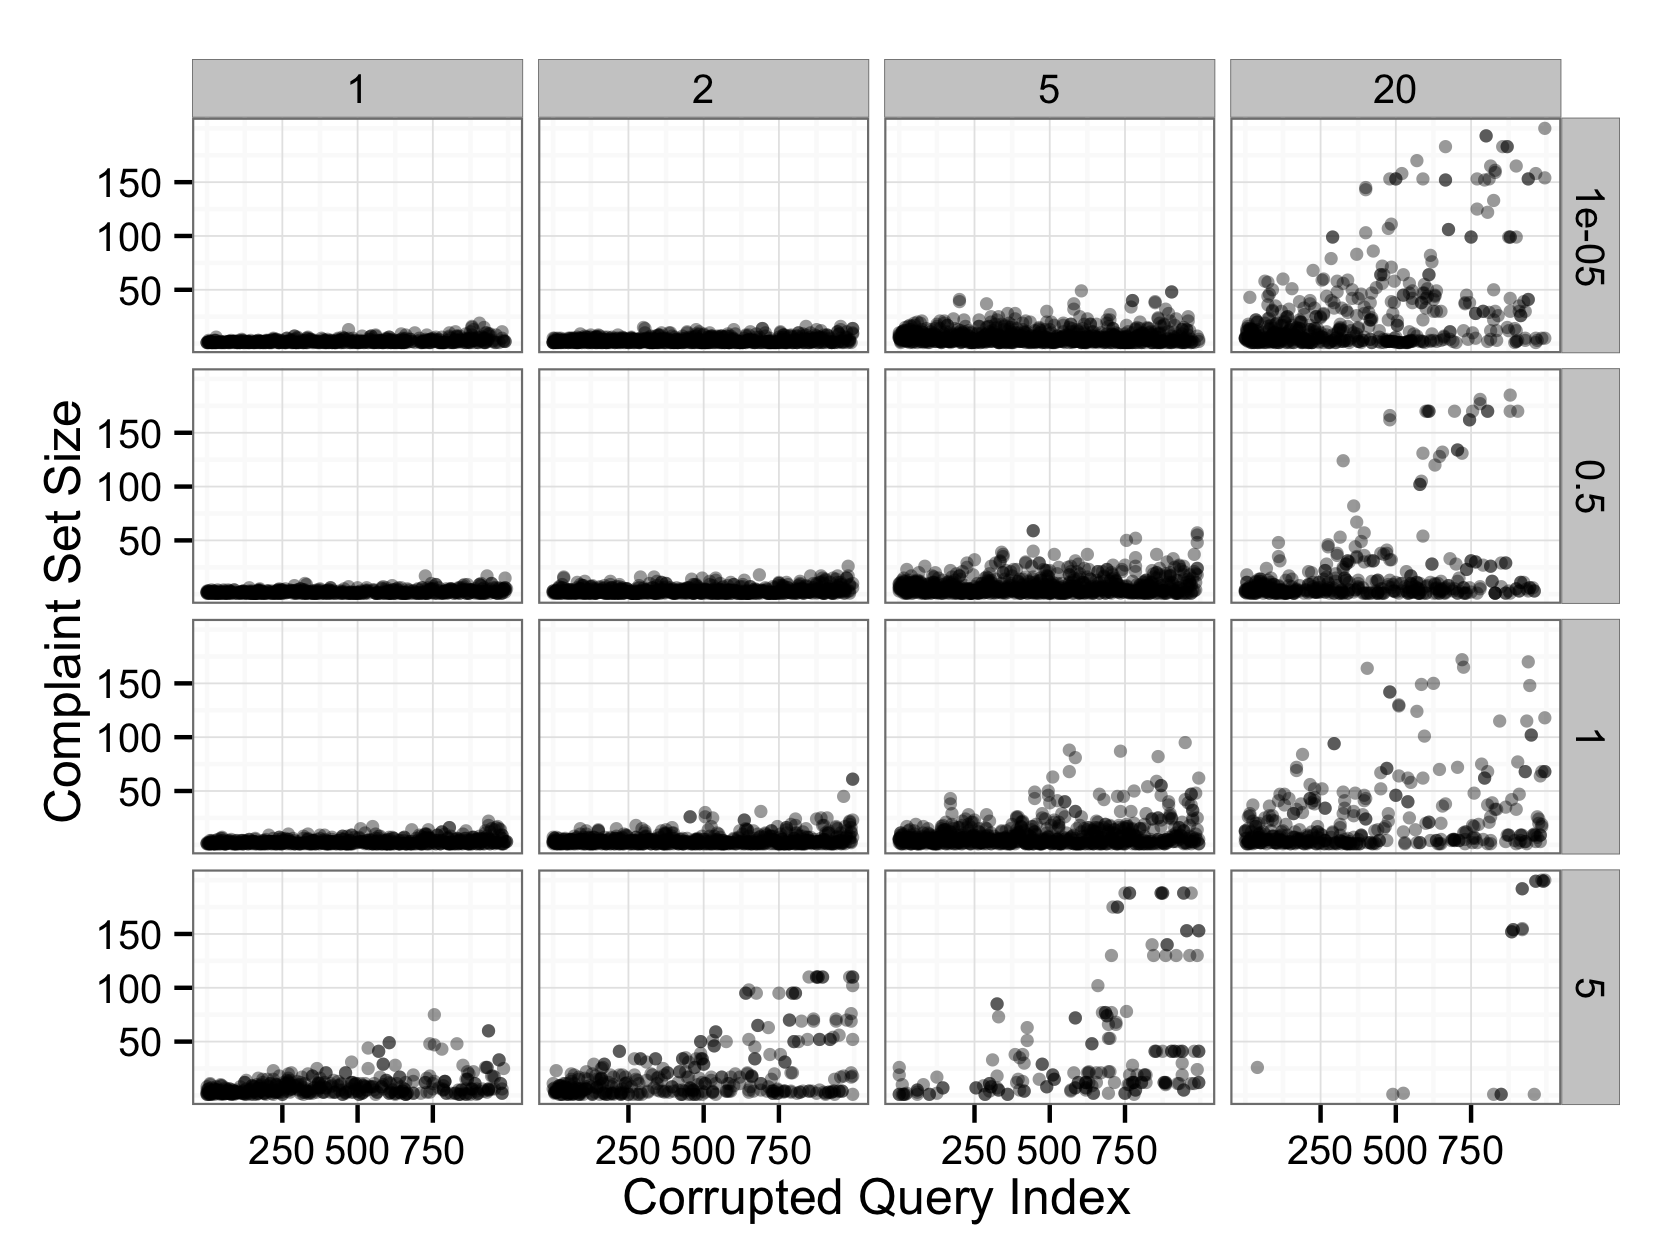
\includegraphics[width = 3in]{figures/qidxsimulation/qidx_v_ncomplaints_20attrs_const}
\caption{Corrupt query index, skew, range vs complaint set size for \textit{constant} \texttt{SET} clauses.}
\label{f:qidx_v_ncomplaints_const} 
\end{figure}

\smallskip
\emph{Constant \texttt{SET} clause: } Figure~\ref{f:qidx_v_ncomplaints_const} plots a representative set of parameters including corrupt query index, range, and skew. We plot one point
for each corrupted query index that results in a complaint set with at least one complaint. 
These results highlight several interesting trends:  With small update range and small skew factor (left upper corner)
the size of the complaint sets are relatively small, and their frequency is constant across the possible query indices.
However as we increase the range and skew, more recent queries are more likely to result in very large complaint sets (at times the size of the database).   
This effect is because the queries that have higher overlap of their \texttt{WHERE} clauses will set groups of tuples to the same value,
and over time, skew the distribution of tuple values to a small number of possible values. 
Thus, more recent corruptions that affect a large cluster of similar tuples will result in a large complaint set.
\ewu{This this effect an artifact of bad experiment design (of our query generation), or is it something that would always happen?  Need to address, since obvious question!}
And the possibility of query overlap increases with update range and skew as these two factors increase the likelihood that queries share the same \texttt{WHERE} and \texttt{SET} clause. 



\begin{figure}[t]
\centering
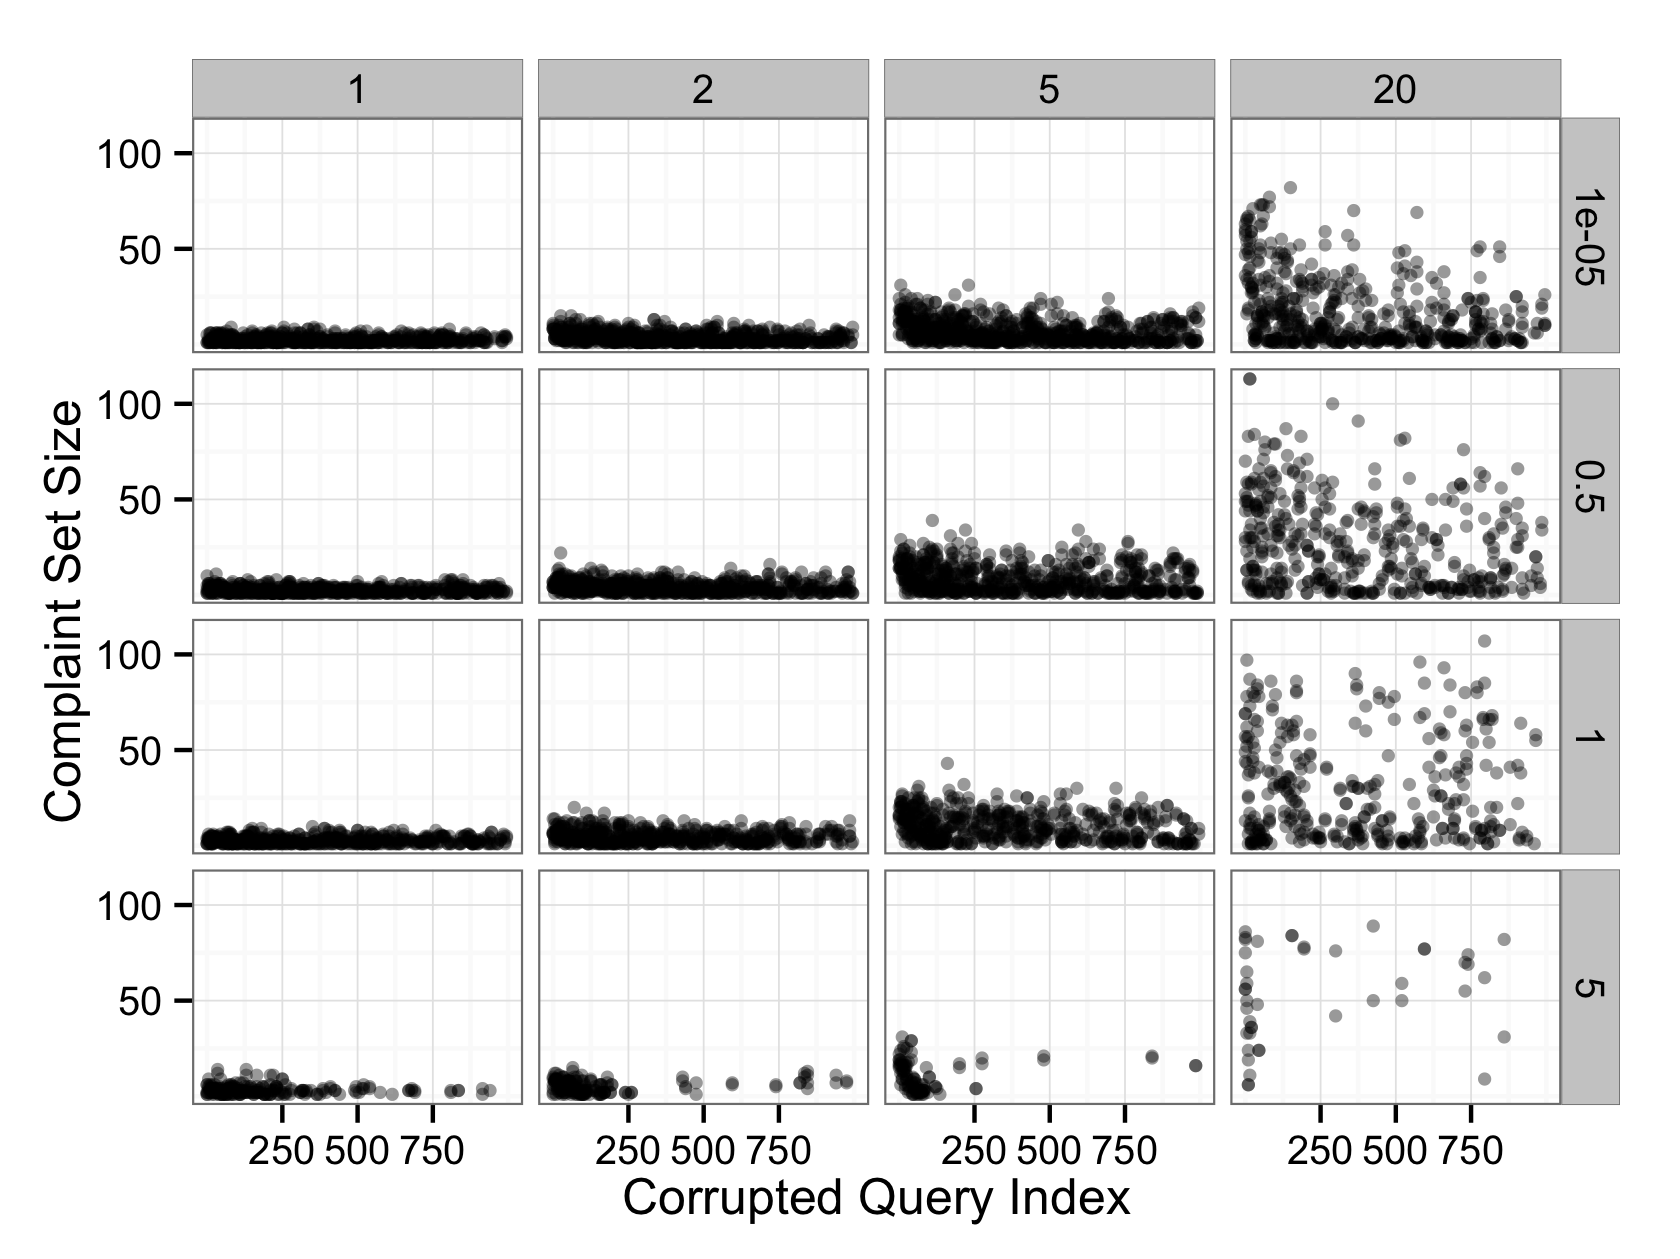
\includegraphics[width = 3in]{figures/qidxsimulation/qidx_v_ncomplaints_20attrs_rel}
\caption{Query index vs complaint set size for $set = rel$.}
\label{f:qidx_v_ncomplaints_rel} 
\end{figure}

\smallskip
\emph{Relative \texttt{SET} clause: } \xlw{In contrast to \textit{constant} \texttt{SET} queries, Figure~\ref{f:qidx_v_ncomplaints_rel} executes the 
same experiment using \textit{relative} \texttt{SET} queries.  In this setting, we find that the trend is
reversed, and older corruptions tend to result in larger complaint sets.  This is because,
subsequent \texttt{UPDATE} queries increment or decrement the attribute value, rather than
overwriting it with a constant value.  The clustering of data values due to query overlap
then increases the number of other tuples affected.
}



\begin{figure*}[ht]
	{\scriptsize
    \begin{minipage}[t]{0.2\textwidth}
         \vspace{0pt} 
         \centering
        \begin{tabular}{lllll}
            \multicolumn{5}{l}{\emph{table}: $D_0$}\\
            \toprule
            \textbf{ID}  & \textbf{$a_1$}    & \textbf{$a_2$} & \textbf{$a_3$} & \textbf{$a_4$} \\
            \midrule
            0 & 8 & 4 & 12 & 28\\
            1 & 2 & 10 & 15 & 3\\
            \bottomrule
            \\
    \end{tabular}
    \end{minipage}
     \begin{minipage}[t]{0.5\textwidth}
         \vspace{0pt} 
         \centering
        \begin{tabular}{l}
            \multicolumn{1}{l}{A \texttt{DELETE} workload  $\mathcal{Q}_{del}$:                                                            }\\
             \toprule
            \texttt{Q1: DELETE FROM table WHERE $a_2$ in \sout{[3,5]} {\color{red}[30, 50]}} \\
   			\texttt{Q2: DELETE FROM table WHERE $a_3$ in [7, 8] }\\ \hline
    \end{tabular}
    \end{minipage}
    \begin{minipage}[t]{0.2\textwidth}
         \vspace{0pt} 
         \centering
       \begin{tabular}{lllll}
            \multicolumn{5}{l}{\emph{table}: $D_1$ after execute $\mathcal{Q}_{del}$}\\
            \toprule
            \textbf{ID}  & \textbf{$a_1$}    & \textbf{$a_2$} & \textbf{$a_3$} & \textbf{$a_4$} \\
            \midrule
            \rowcolor{mid-gray}
            \sout{0} & \sout{8} & \sout{4} & \sout{12} & \sout{28}\\
            1 & 2 & 10 & 15 & 3\\
            \bottomrule
            \\
\end{tabular}
    \end{minipage} \\
  \begin{minipage}[t]{0.2\textwidth}
         \vspace{0pt} 
         \centering
        \begin{tabular}{lllll}
        
            
    \end{tabular}
    \end{minipage}
 \begin{minipage}[t]{0.5\textwidth}
         \vspace{0pt} 
         \centering
        \begin{tabular}{l}
   			\multicolumn{1}{l}{A \texttt{UPDATE} workload $\mathcal{Q}_{up}$:                              }\\
   			 \toprule
            \texttt{Q1: UPDATE table SET $a_1$ = 10 WHERE $a_2$ in \sout{[3,5]} {\color{red}[30, 50]}} \\
   			\texttt{Q2: UPDATE table SET $a_4$ = 7 WHERE $a_3$ in [7, 8] }\\ \hline
            \\
    \end{tabular}
    \end{minipage}     
    \begin{minipage}[t]{0.2\textwidth}
         \vspace{0pt} 
         \centering
\begin{tabular}{lllll}
            \multicolumn{5}{l}{\emph{table}: $D_1'$ after execute $\mathcal{Q}_{up}$}\\
            \toprule
            \textbf{ID}  & \textbf{$a_1$}    & \textbf{$a_2$} & \textbf{$a_3$} & \textbf{$a_4$} \\
            \midrule
            \rowcolor{mid-gray}
            0 & \color{red}{8} & 4 & 12 & 28\\
            1 & 2 & 10 & 15 & 3\\
            \bottomrule
            \\
\end{tabular}
    \end{minipage}
}
    \vspace{-2mm}
    \caption{A initial database state $D_0$ and database states after apply $\mathcal{Q}_{del}$ and $\mathcal{Q}_{up}$ on $D_0$. }
    \label{fig:example2}
\end{figure*}
\section{Repairing the Correct Query}
\label{app:index}

The experimental section (Section~\ref{sec:experiments}) primarily focused on performance and accuracy measures of the repairs, and for space constraints, ignored 
whether the proposed repair was actually the correct query (it is possible we fix an incorrect query in a way that resolves the complaint set).
Although we found in most circumstances we identify the correct query to fix, we now turn our attention to better understand 
the conditions when we may fix the incorrect query. 

   \begin{figure*}[t]
  \centering
  \begin{subfigure} [t]{.3\textwidth}
    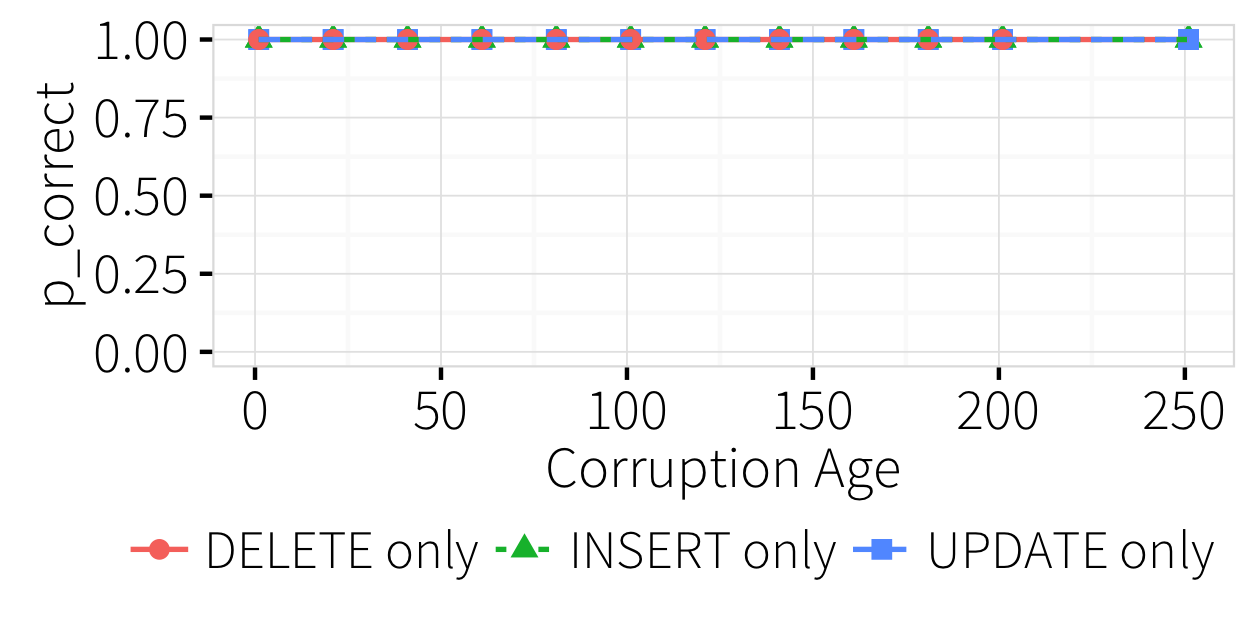
\includegraphics[width = .99\columnwidth]{figures/indelup_acc_idx}
    \vspace*{-.25in}
    \caption{Correct repair ratio vs. query types}
    \label{f:querytyperatio} 
    \end{subfigure}
    \begin{subfigure} [t]{.3\textwidth}
    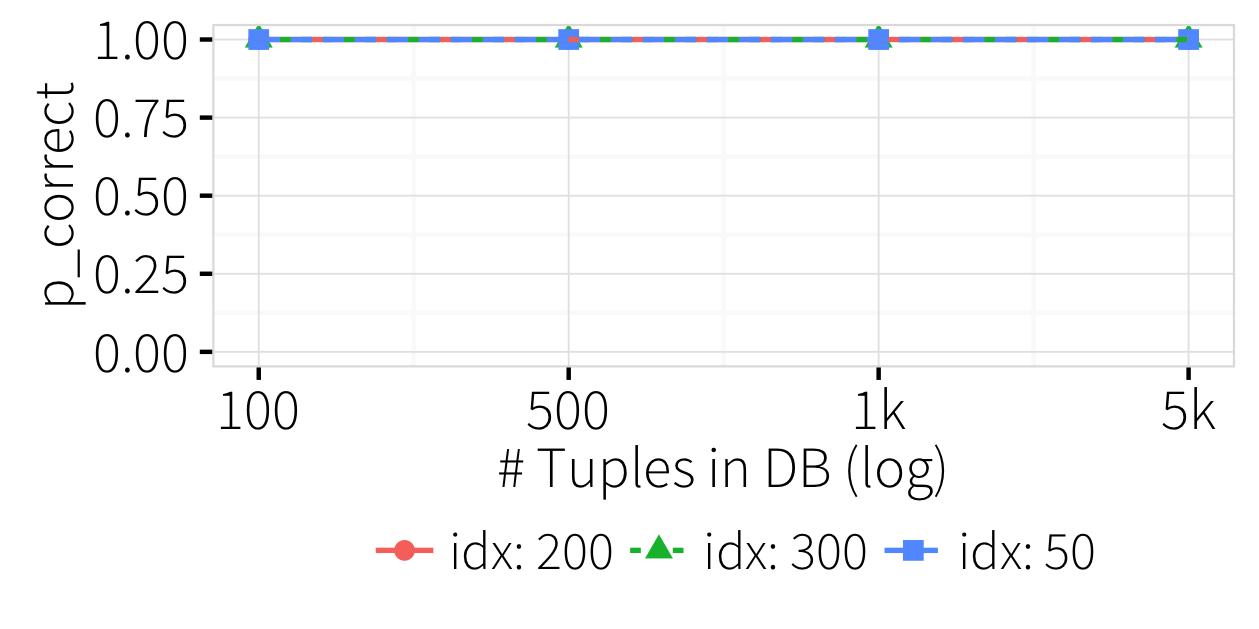
\includegraphics[width = .99\columnwidth]{figures/dbsize_acc_idx}
    \vspace*{-.25in}
    \caption{Correct repair ratio vs. database sizes}
    \label{f:dbsizeratio} 
    \end{subfigure}
    \begin{subfigure} [t]{.3\textwidth}
    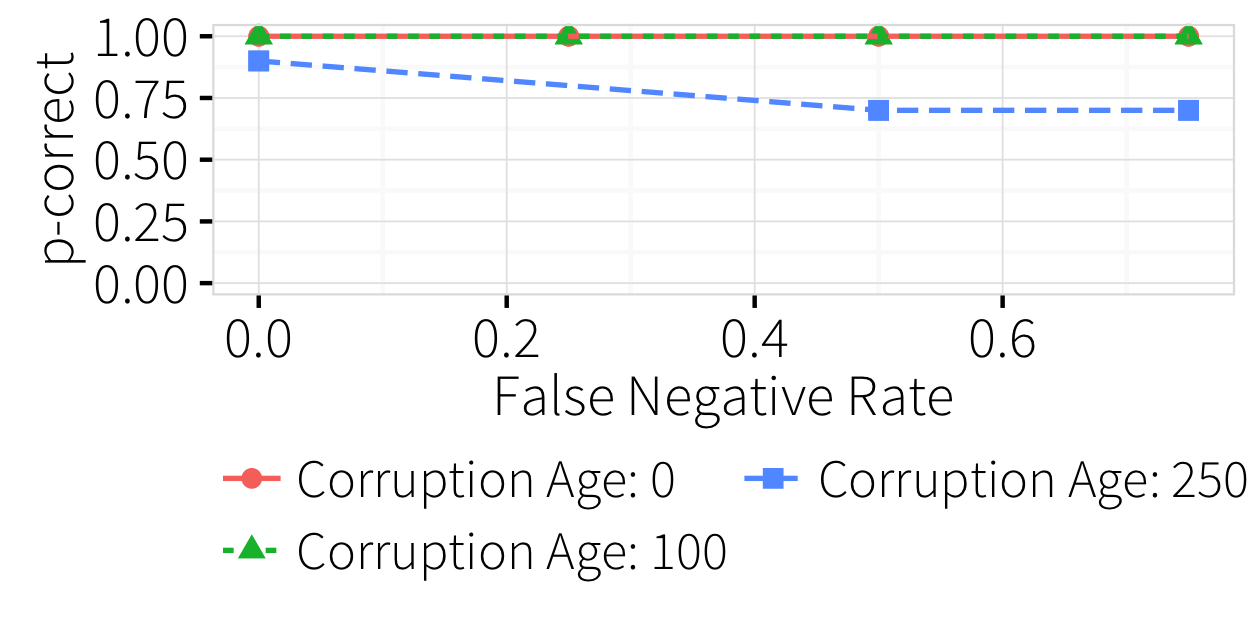
\includegraphics[width = .99\columnwidth]{figures/noise_fn_acc_idx}
    \vspace*{-.25in}
    \caption{Correct repair ratio vs. false negatives}
    \label{f:fnratio} 
    \end{subfigure} \\
    \begin{subfigure} [t]{.3\textwidth}
    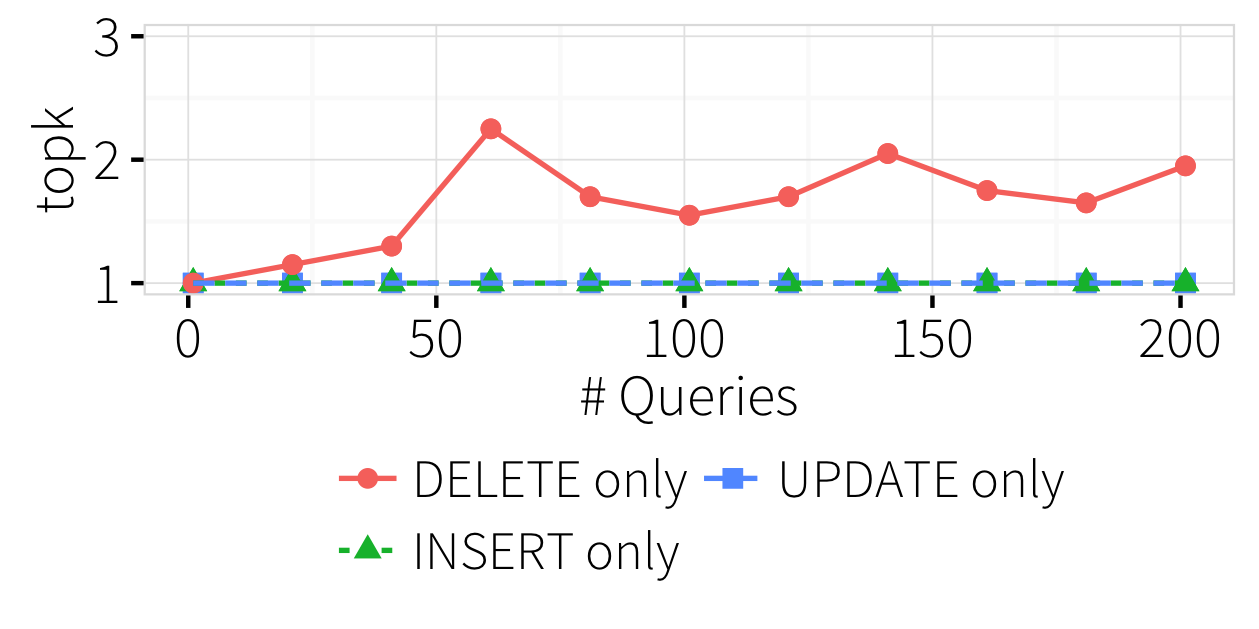
\includegraphics[width = .99\columnwidth]{figures/indelup_fixcount}
    \vspace*{-.25in}
    \caption{Top-k vs. query types. }
    \vspace*{-.1in}
    \label{f:querytypefixcount} 
    \end{subfigure}
    \begin{subfigure} [t]{.3\textwidth}
    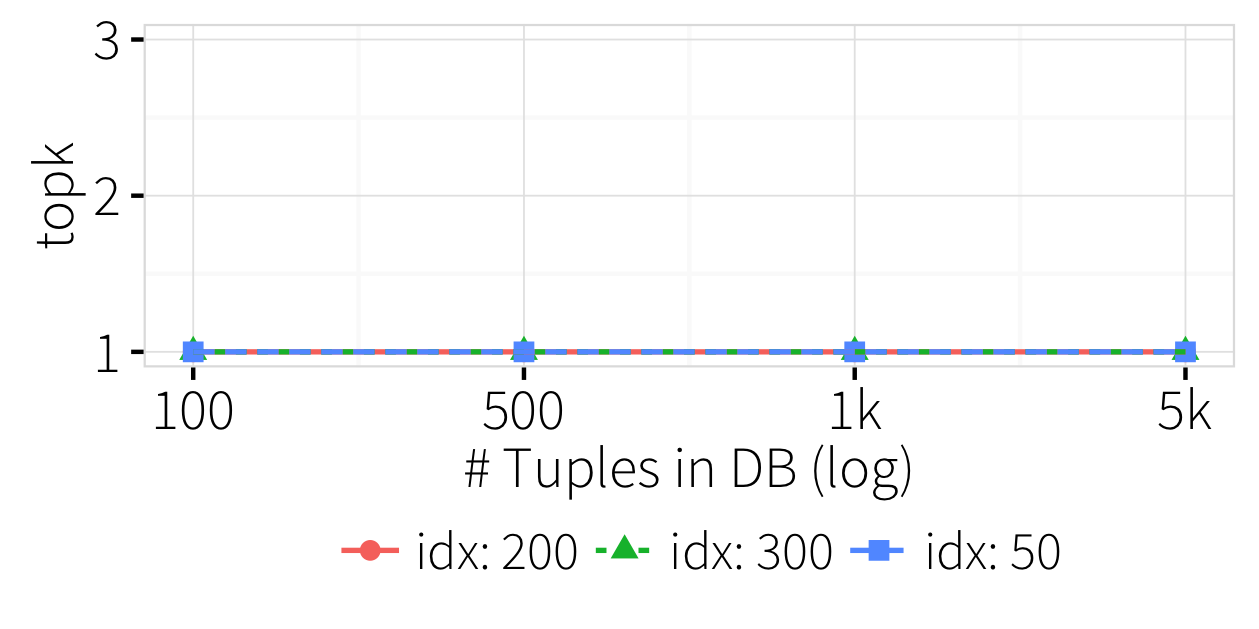
\includegraphics[width = .99\columnwidth]{figures/dbsize_fixcount}
    \vspace*{-.25in}
    \caption{Top-k vs. database sizes. }
    \vspace*{-.1in}
    \label{f:dbsizecount} 
    \end{subfigure}
    \begin{subfigure} [t]{.3\textwidth}
    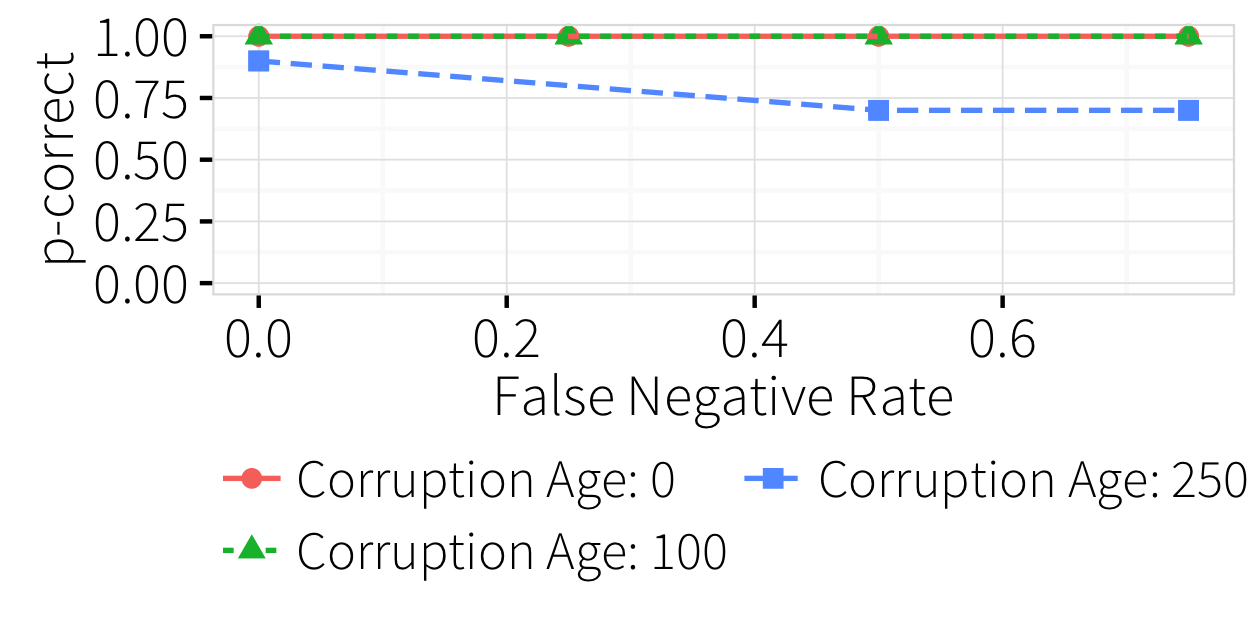
\includegraphics[width = .99\columnwidth]{figures/noise_fn_acc_idx}
    \vspace*{-.25in}
    \caption{Top-k vs. false negatives (\color{red}{not complete!})}
    \vspace*{-.1in}
    \label{f:fnfixcount} 
    \end{subfigure}
   \caption{Correct repair ratio and number of candidate fixes of \sys varies on different types of workloads and false negative rate but remain 
   stable for with increasing number of tuples on \texttt{UPDATE} workload.}
   \vspace*{-.1in}
   \label{fig:truerate}
  \end{figure*}


\subsection{Experimental Results}
To evaluate \sys's ability in identifying the correct query to fix, we execute QFix over 20 random runs and summarize our results using two evaluation metrics:
The first $p_{correct}$ computes the ratio between the number of runs where \sys correctly repairs the corrupt query and where \sys
repairs the wrong query; The second metric $topk$ measures the number of repairs that \sys proposes before repairing the true corrupt query.
The second metric is useful to quantify the extent that \sys's repairs are false positives (though they may correctly resolve the complaint set).
A small $topk$ value suggests that \sys is still effective at providing repair \emph{recommendations} as part of a diagnostic interface.

\textbf{Correct repair ratio vs. query types: } In Figure~\ref{f:querytyperatio}, we first evaluate $p_{correct}$ rate on three types of workloads: \sys identifies the correct query to fix ($p_{correct} = 1.0$ and $topk = 1$) for \texttt{UPDATE} and \texttt{INSERT} workloads but unstable and much lower rate for \texttt{DELETE} workload. This is expected since more information of the actual incorrectness get maintained through \texttt{UPDATE} queries by the updated tuple values. \ewu{Is this because the problem is fundamentally underconstrained?  if so, explain in those terms and describe why.} However, such information get lost and obscured for \texttt{DELETE} queries as those deleted tuples no longer exist in the database. As a result, actual incorrect queries in \texttt{UPDATE} workloads are much easier to identify than those in \texttt{DELETE} workloads. \texttt{INSERT} workloads are easy to fix by natural since each \texttt{INSERT} query only touches one tuple. 

To further illustrate this, we present the following toy example (Figure~\ref{fig:example2}) of two simple query logs, one for \texttt{DELETE} workload and one for \texttt{UPDATE} workload, that operate on the same initial database state and with the exact same \texttt{WHERE} clauses. 

In the above example, we find that there exist two candidate fixes for the \texttt{DELETE} workload $\mathcal{Q}_{del}$: one can either modify the \texttt{WHERE} clause of $Q2$ to $[12, 12]$ or the \texttt{WHERE} clause of $Q1$ to $[4, 4]$. In addition, the two candidate fixes achieve the exact same final database state. However, there only exists one candidate fix for the \texttt{UPDATE} workload $\mathcal{Q}_{up}$ since values in every attribute must satisfy with the desired database state. According to the converted constraints, modifying $Q2$ cannot solve the problem since it would not fix the value in the incorrect attribute $a_1$.  

\textbf{Top-k vs. query types: } In Figure~\ref{f:querytypefixcount}, we observe the same trend: the $topk$ count for \texttt{UPDATE} and \texttt{INSERT} workloads remain $1$ across all query indexes while the $topk$ count shows unstable and much higher value for \texttt{DELETE} workloads. Overall, we find \sys above is able to find the true repair within 3 diagnosis over more than 85\% of all random runs. 

\textbf{Correct repair ratio \& top-k vs. database sizes: } We next narrow down to \texttt{UPDATE} workload and evaluate \sys's behavior with increasing amount of tuples in the database. We observe $p_{correct} = 1$ and $topk = 1$ on different corrupt indexes in all database sizes (Figure~\ref{f:dbsizeratio}~\ref{f:dbsizecount}). 

\textbf{Correct repair ratio \& top-k vs. false negatives: } We finally evaluate \sys on \texttt{UPDATE} workload with increasing false negative rates. Similar to the quality drop in Figure~\ref{f:falsenegative_acc}, we observe the $p_{correct}$ (Figure~\ref{f:fnratio}) rate also suffers from less submitted complaints when errors happen early in the query log. However, \sys achieves above $0.75$ $p_{correct}$ rate for more recent errors (corrupt index is 300 and 200) even with high false negative rate. The $topk$ behaves similar to $p_{correct}$ in which $topk$ increasing with the false negative rate (Figure~\ref{f:fnfixcount}).  
\fi}





